\subsection{Deductive Reasoning and Logical Connectives}
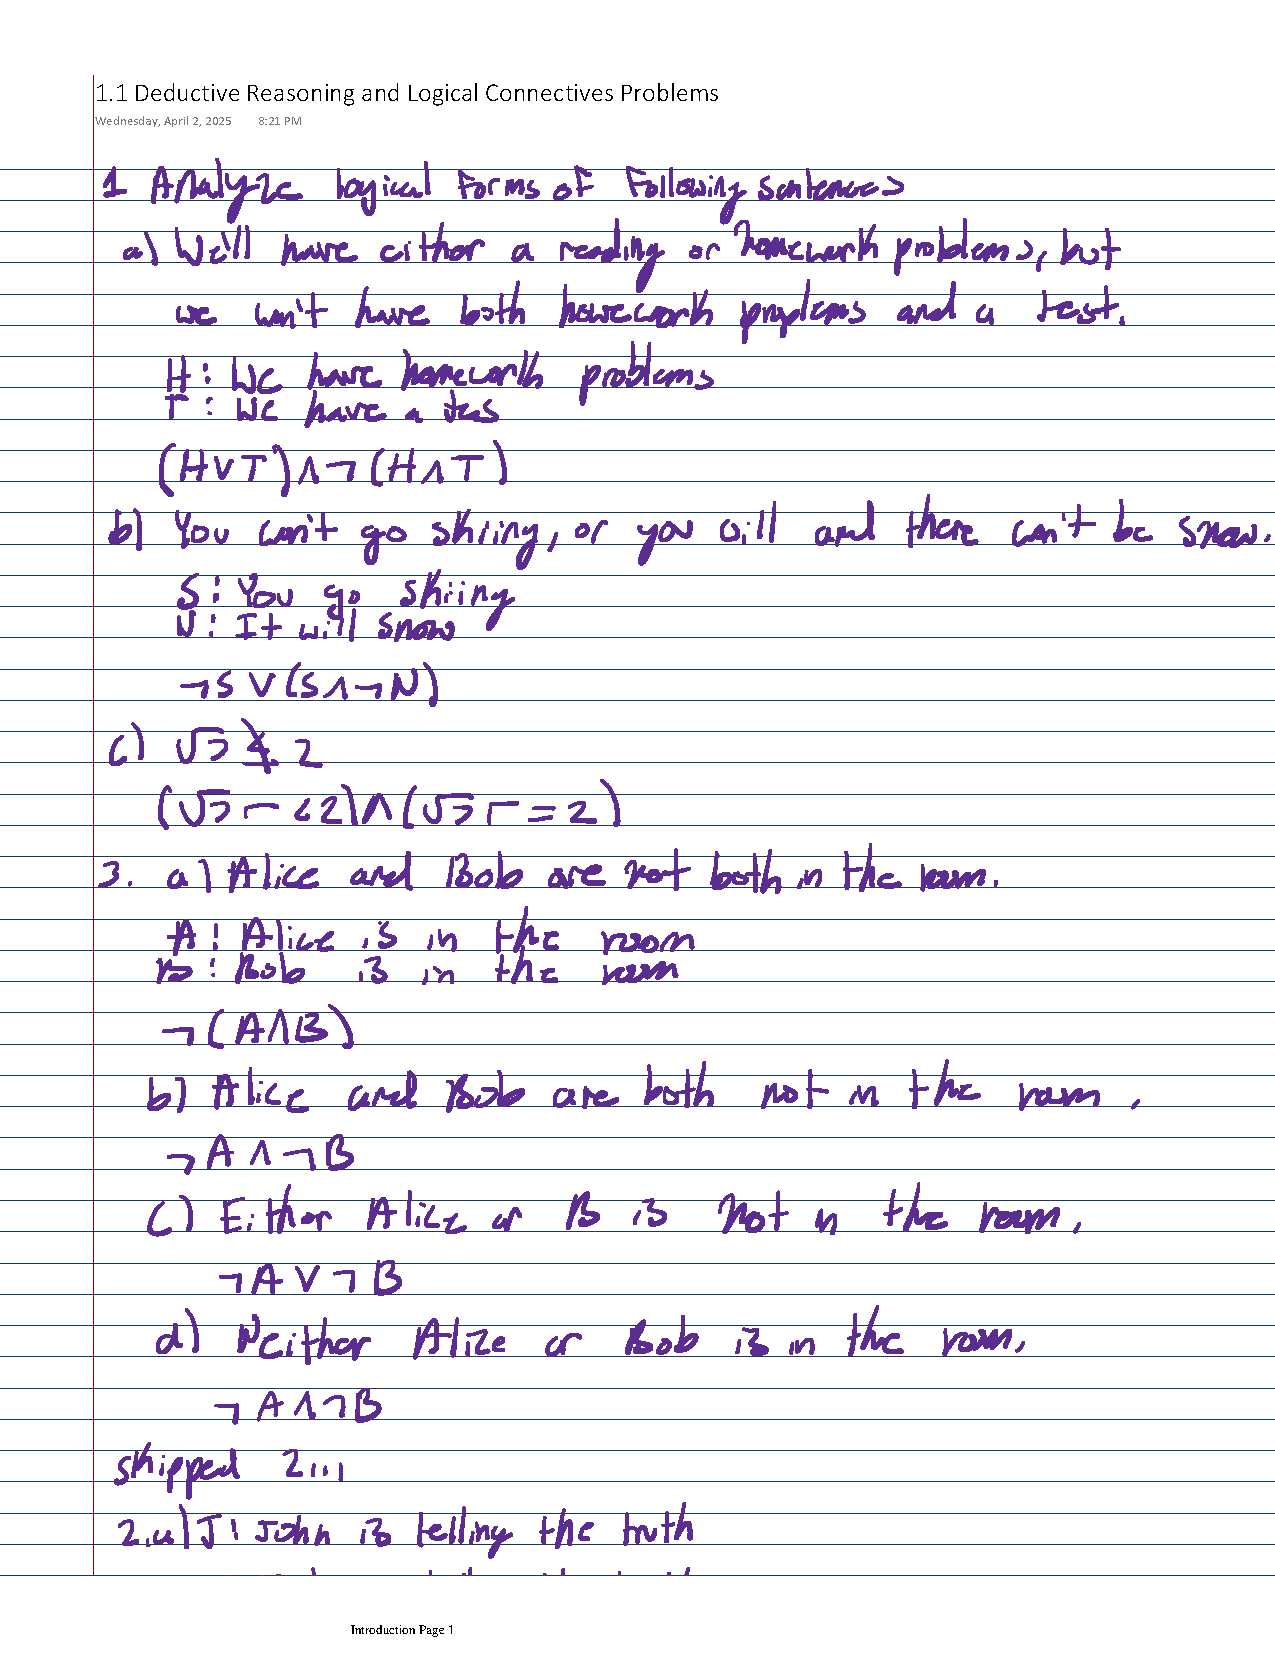
\includepdf[pages={1-5}]{misc/1.1.pdf}

\subsection{Truth Tables}
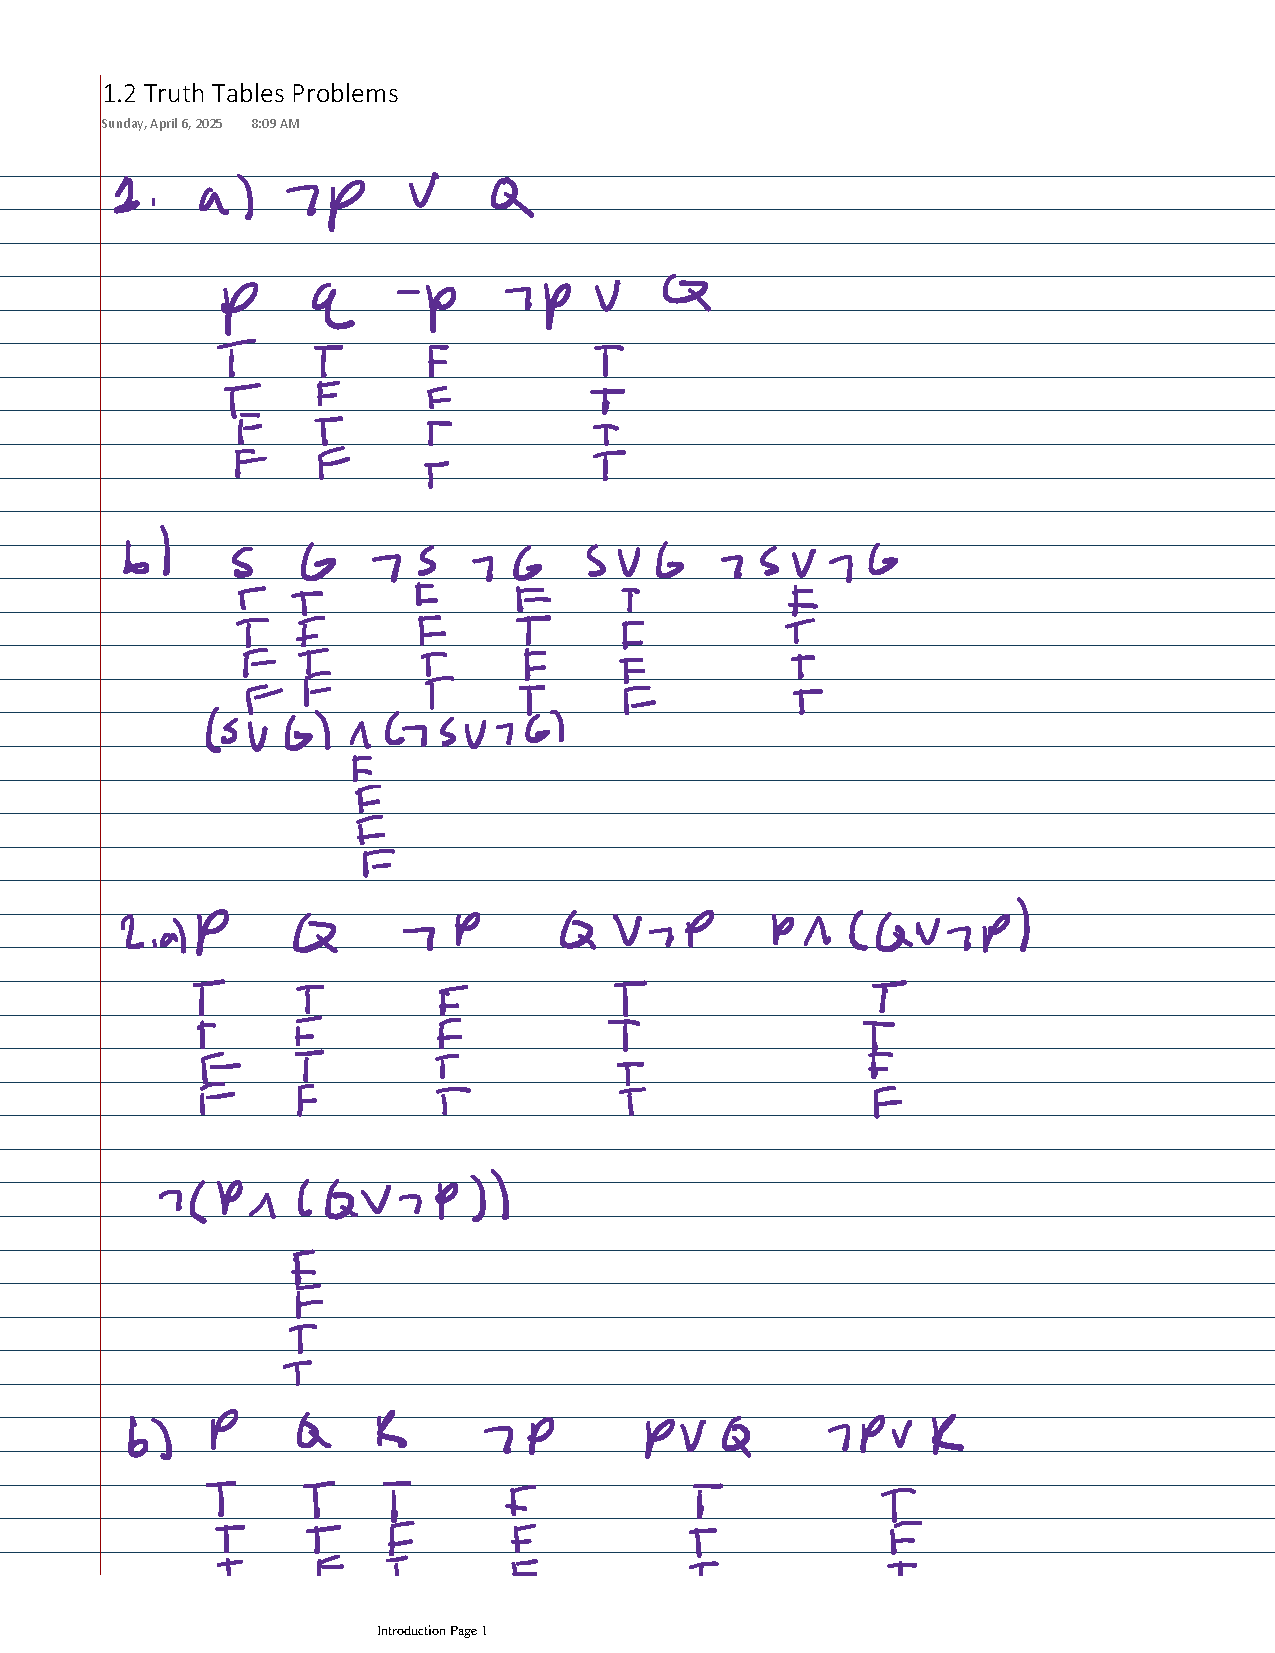
\includepdf[pages={1-6}]{misc/1.2.pdf}

\textbf{Problem 9:}
\begin{figure}[H]
    \centering
    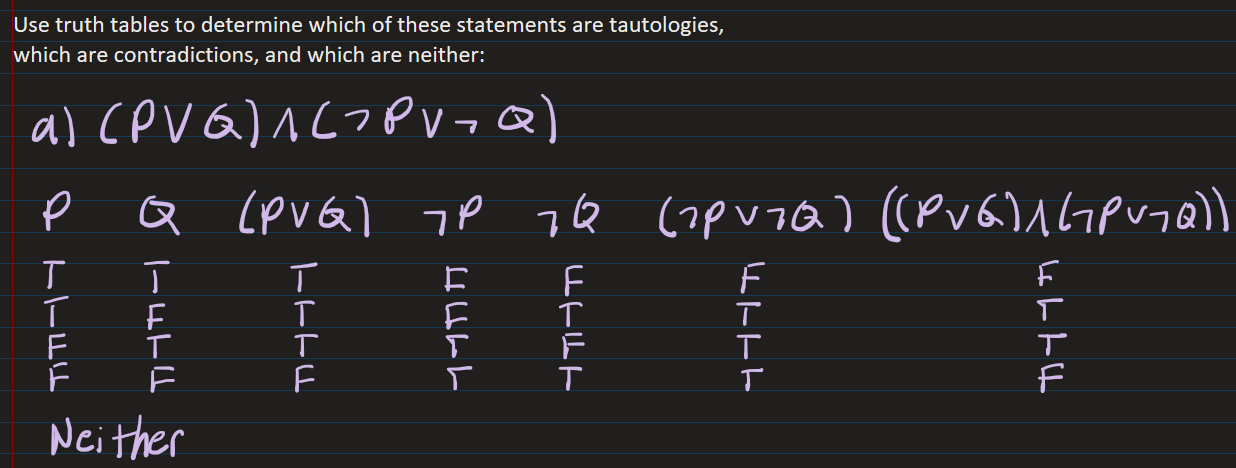
\includegraphics[width=0.8\textwidth]{images/1.2/1.PNG}
\end{figure}
\begin{figure}[H]
    \centering
    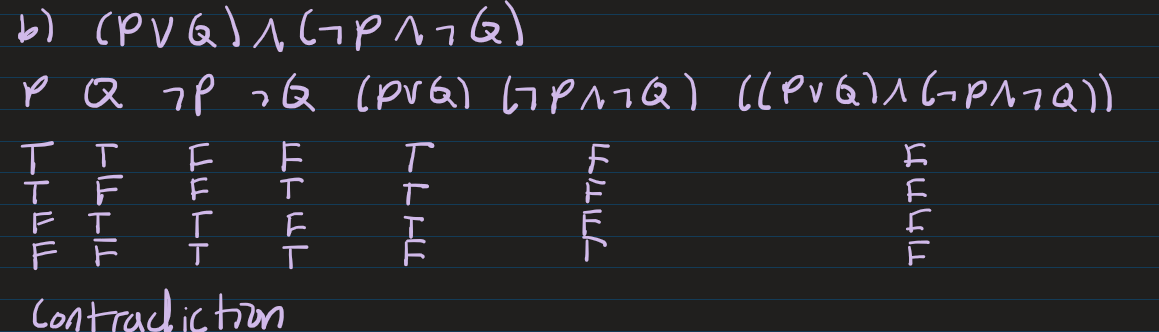
\includegraphics[width=0.8\textwidth]{images/1.2/2.PNG}
\end{figure}
\begin{figure}[H]
    \centering
    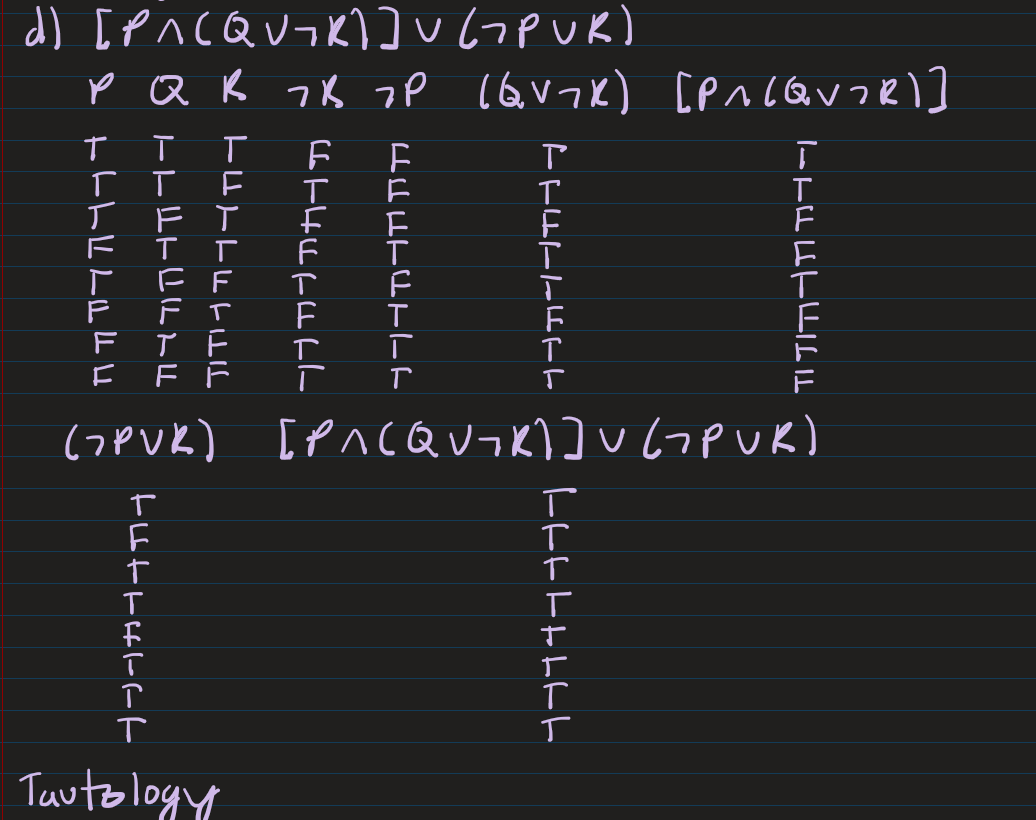
\includegraphics[width=0.8\textwidth]{images/1.2/3.PNG}
\end{figure}

\textbf{Problem 10:}
\begin{figure}[H]
    \centering
    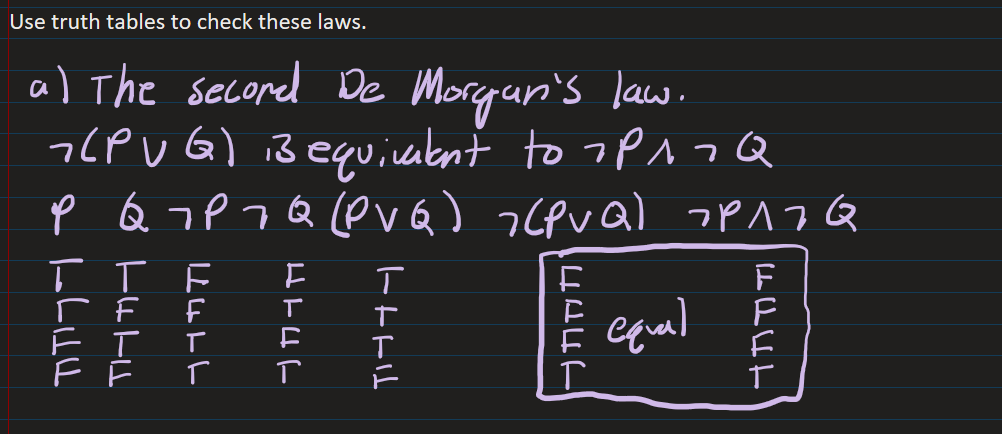
\includegraphics[width=0.8\textwidth]{images/1.2/4.PNG}
\end{figure}
\begin{figure}[H]
    \centering
    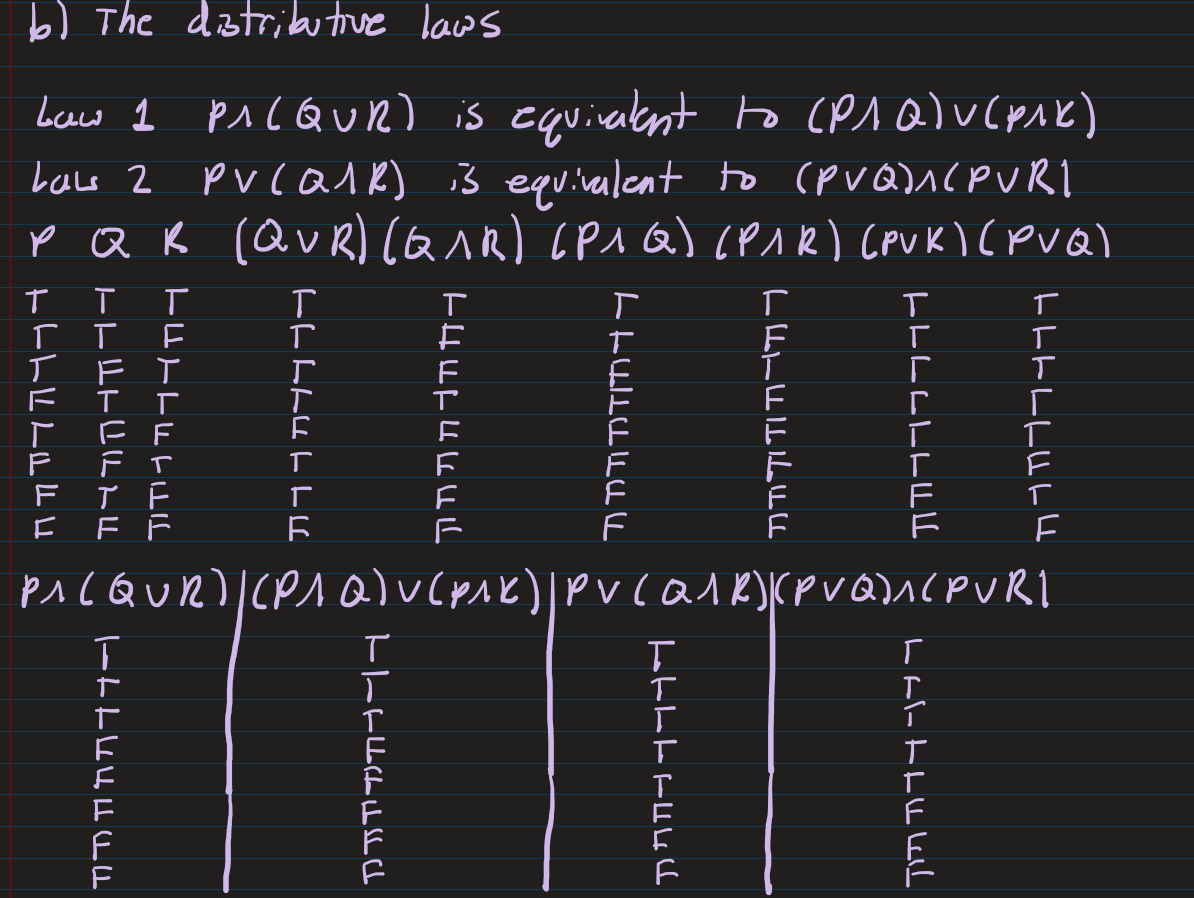
\includegraphics[width=0.8\textwidth]{images/1.2/5.PNG}
\end{figure}


\textbf{Problem 12:}
\begin{figure}[H]
    \centering
    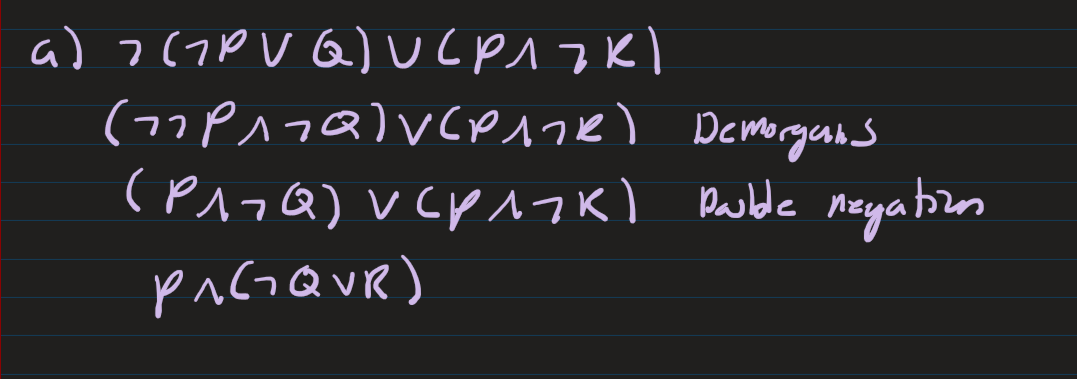
\includegraphics[width=0.8\textwidth]{images/1.2/6.PNG}
\end{figure}
\begin{figure}[H]
    \centering
    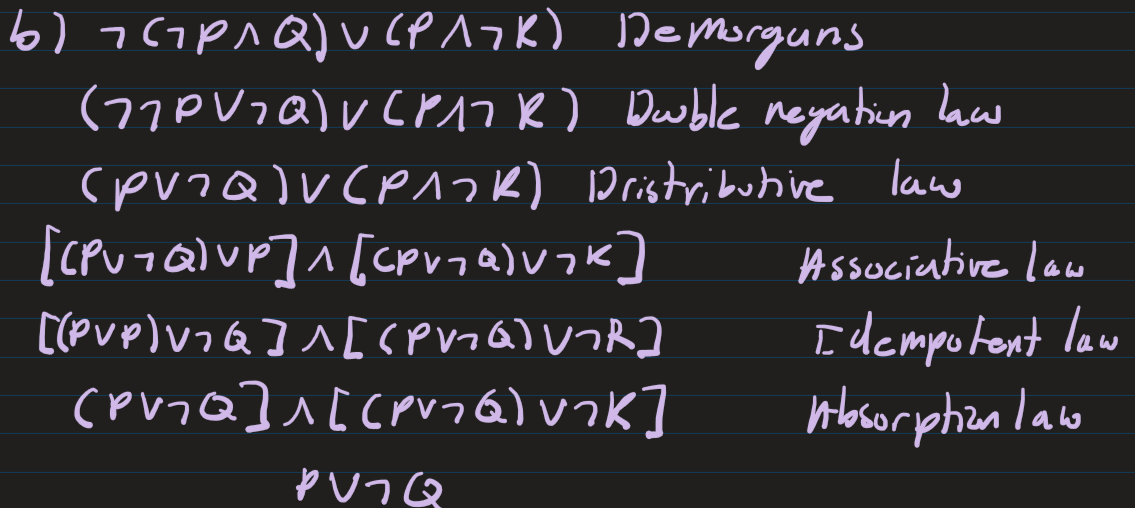
\includegraphics[width=0.8\textwidth]{images/1.2/7.PNG}
\end{figure}
\begin{figure}[H]
    \centering
    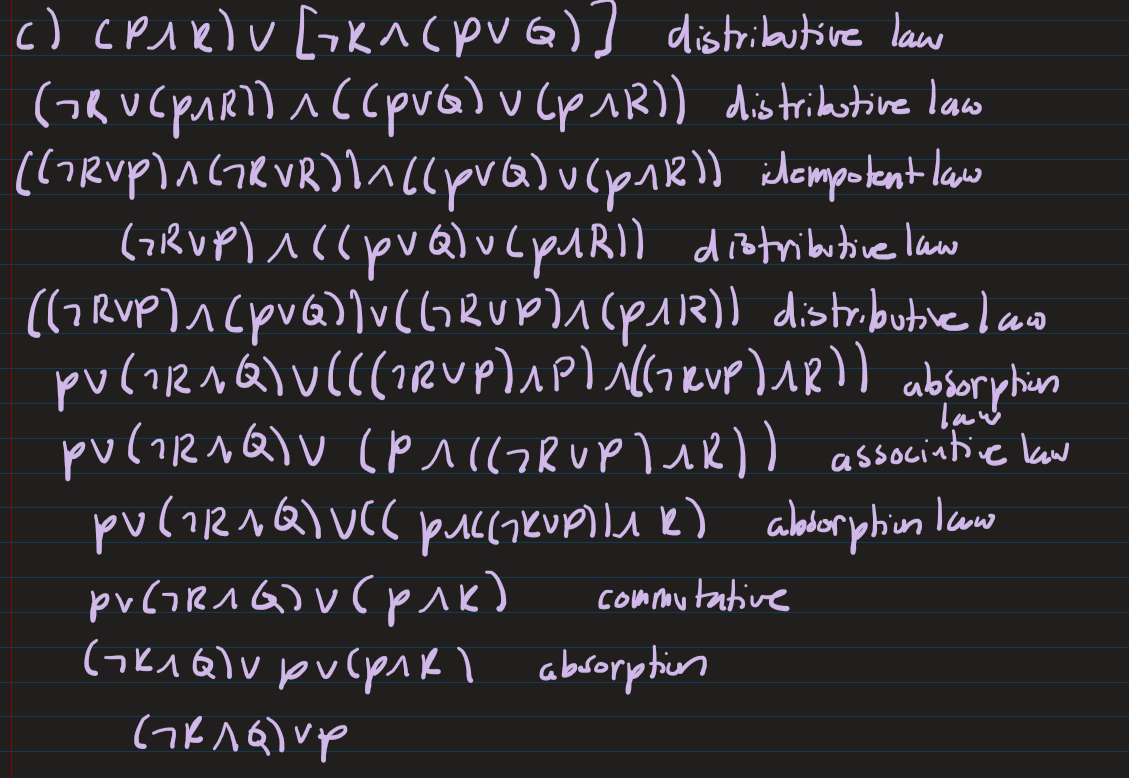
\includegraphics[width=0.8\textwidth]{images/1.2/8.PNG}
\end{figure}

\textbf{Problem 13:}
\begin{figure}[H]
    \centering
    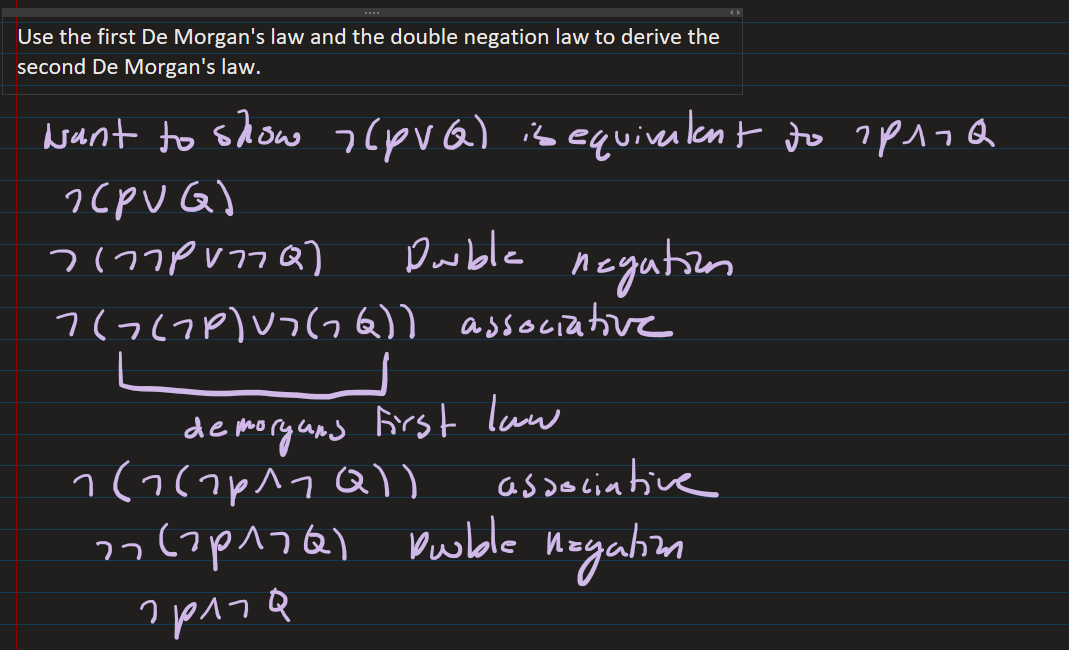
\includegraphics[width=0.8\textwidth]{images/1.2/9.PNG}
\end{figure}

\textbf{Problem 14:}
\begin{figure}[H]
    \centering
    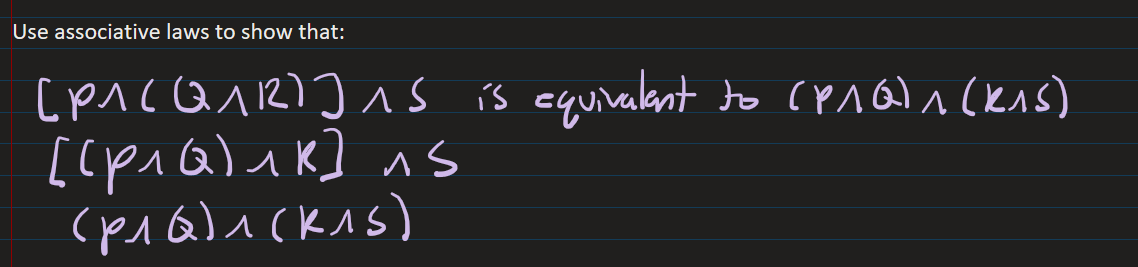
\includegraphics[width=0.8\textwidth]{images/1.2/10.PNG}
\end{figure}

\textbf{Problem 15:}
\begin{figure}[H]
    \centering
    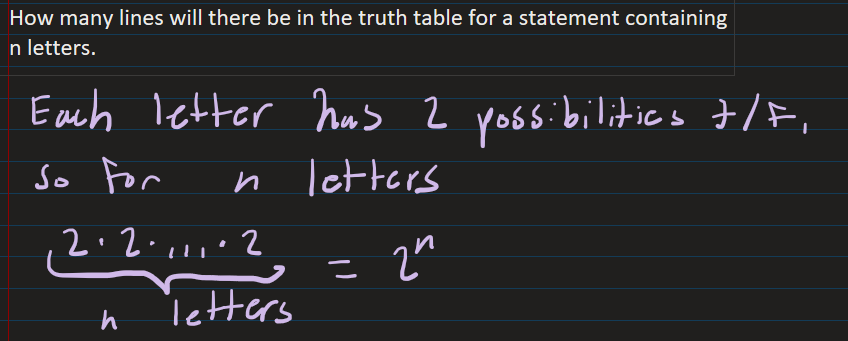
\includegraphics[width=0.8\textwidth]{images/1.2/11.PNG}
\end{figure}

\textbf{Problem 16:}
\begin{figure}[H]
    \centering
    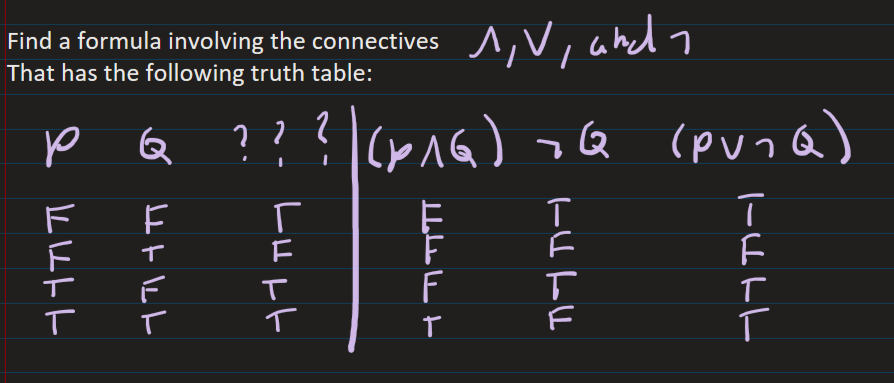
\includegraphics[width=0.8\textwidth]{images/1.2/12.PNG}
\end{figure}

\textbf{Problem 17:}
\begin{figure}[H]
    \centering
    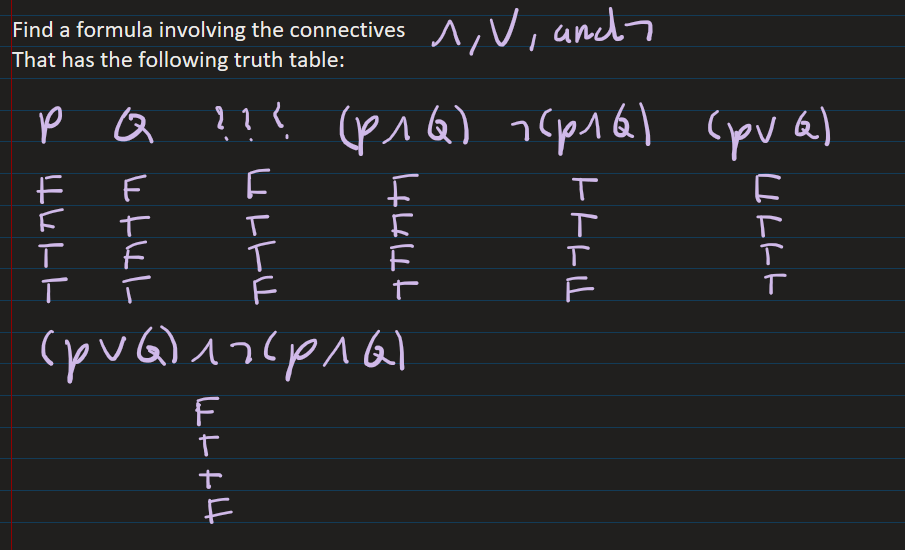
\includegraphics[width=0.8\textwidth]{images/1.2/13.PNG}
\end{figure}

\textbf{Problem 18:}
\begin{figure}[H]
    \centering
    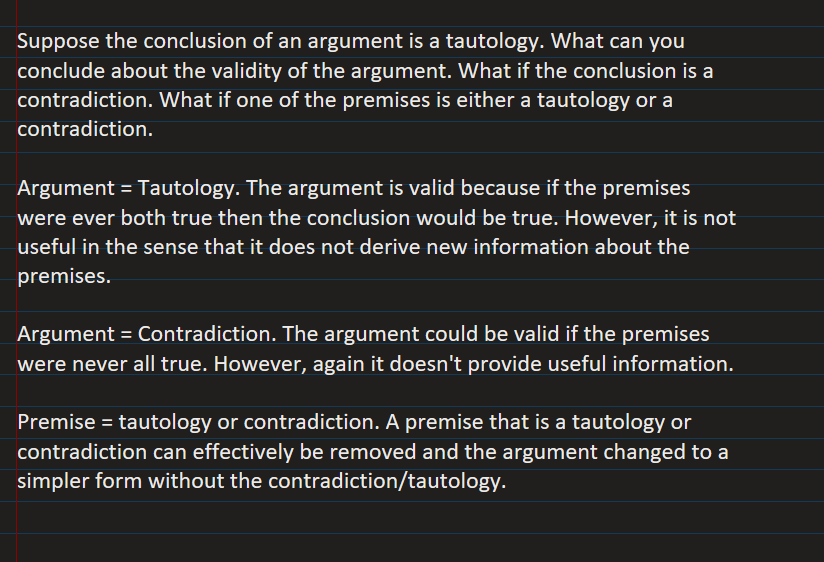
\includegraphics[width=0.8\textwidth]{images/1.2/14.PNG}
\end{figure}

\subsection{Variables and Sets}

\textbf{Problem 1:}
\begin{figure}[H]
    \centering
    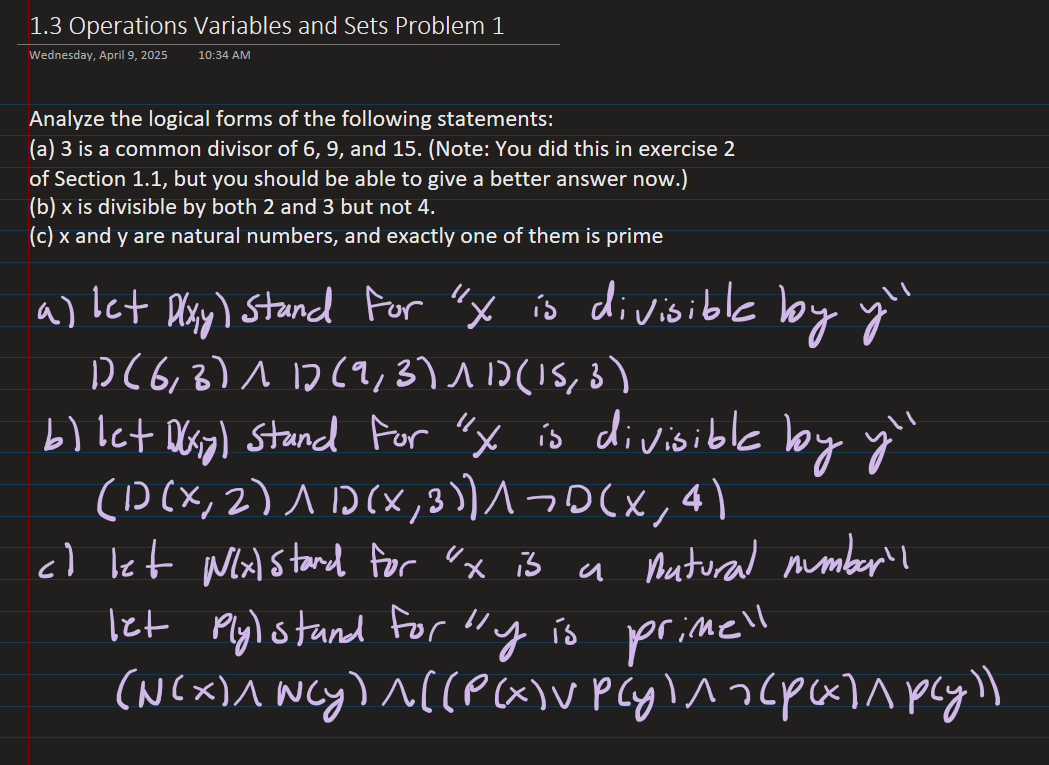
\includegraphics[width=0.8\textwidth]{images/1.2/15.PNG}
\end{figure}

\textbf{Problem 2:}
\begin{figure}[H]
    \centering
    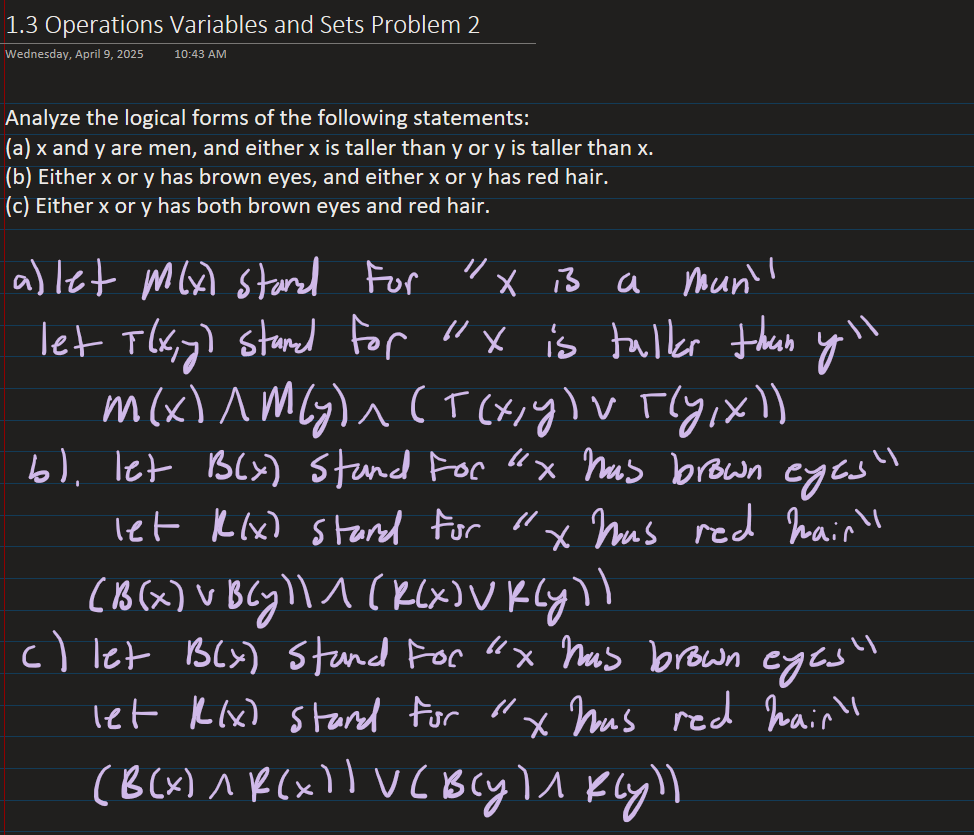
\includegraphics[width=0.8\textwidth]{images/1.2/16.PNG}
\end{figure}

\textbf{Problem 3:}
\begin{figure}[H]
    \centering
    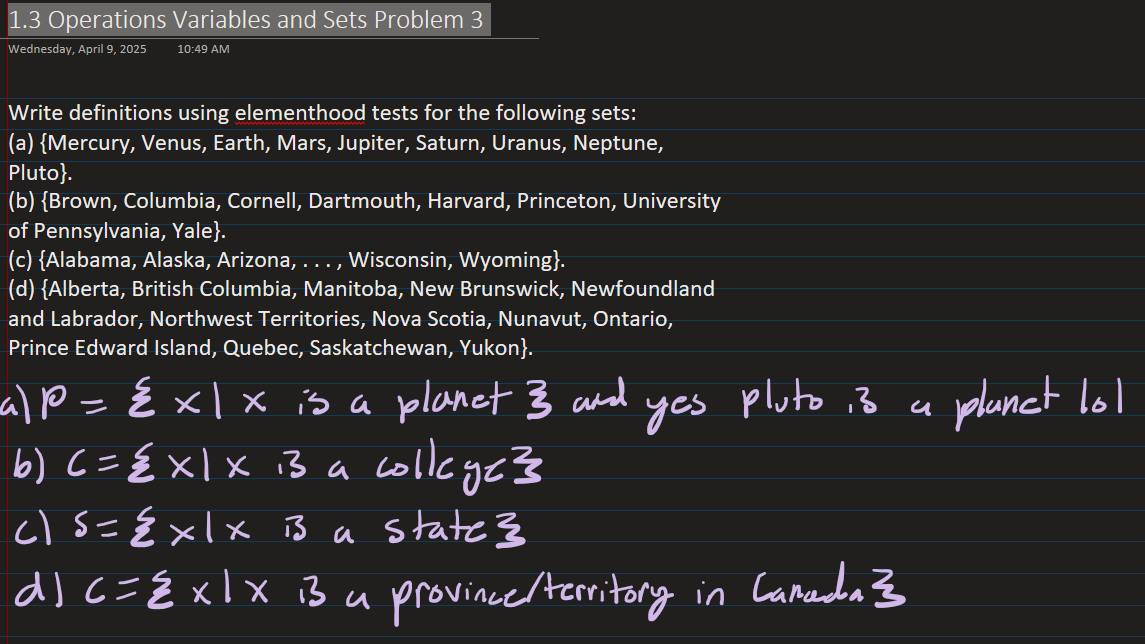
\includegraphics[width=0.8\textwidth]{images/1.2/17.PNG}
\end{figure}

\textbf{Problem 4:}
\begin{figure}[H]
    \centering
    
\includegraphics[width=0.8\textwidth]{images/1.2/18.PNG}
\end{figure}
\begin{figure}[H]
    \centering
    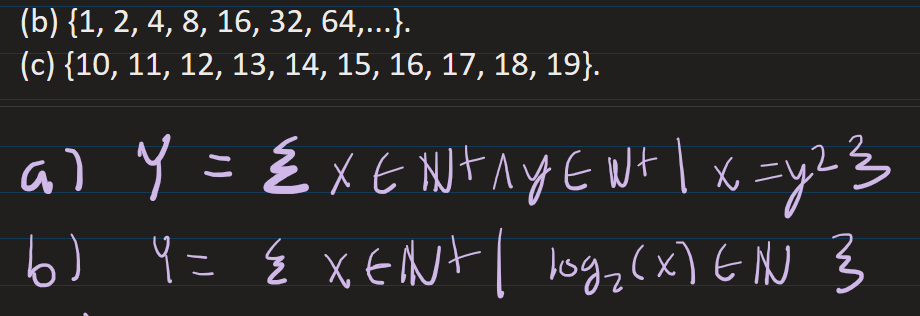
\includegraphics[width=0.8\textwidth]{images/1.2/19.PNG}
\end{figure}

\textbf{Problem 5:}
\begin{figure}[H]
    \centering
    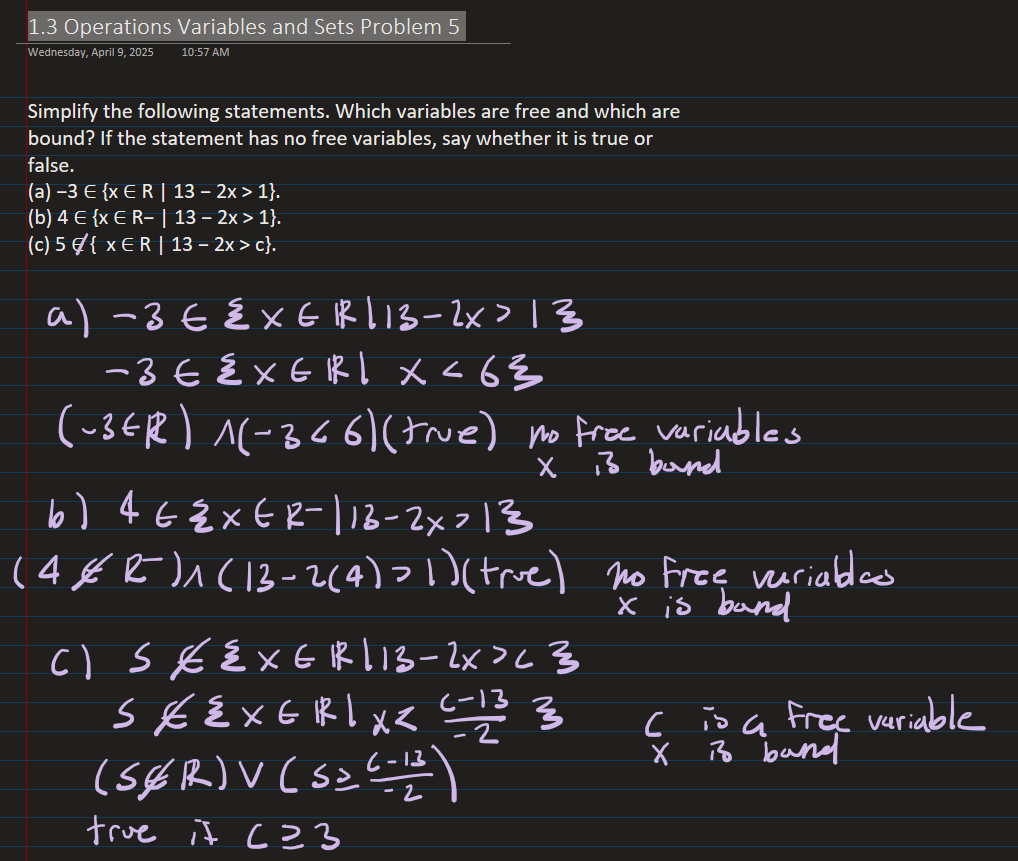
\includegraphics[width=0.8\textwidth]{images/1.2/20.PNG}
\end{figure}

\textbf{Problem 6:}
\begin{figure}[H]
    \centering
    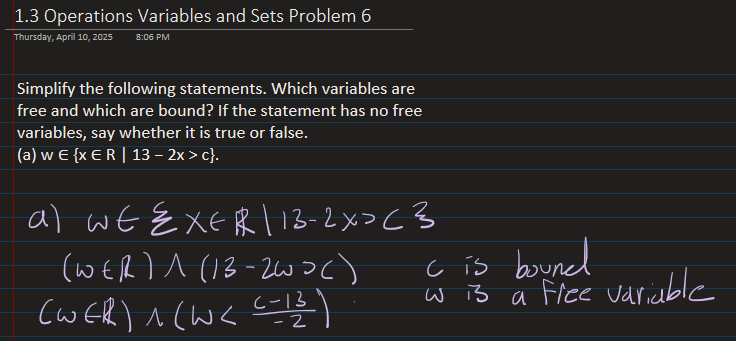
\includegraphics[width=0.8\textwidth]{images/1.2/21.PNG}
\end{figure}
\begin{figure}[H]
    \centering
    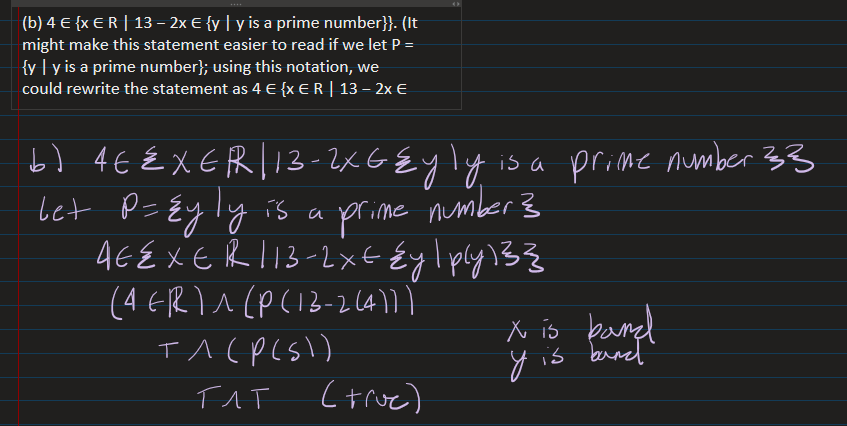
\includegraphics[width=0.8\textwidth]{images/1.2/22.PNG}
\end{figure}
\begin{figure}[H]
    \centering
    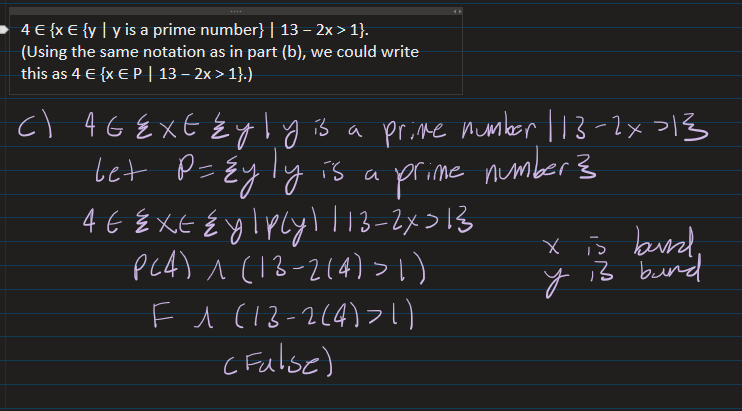
\includegraphics[width=0.8\textwidth]{images/1.2/23.PNG}
\end{figure}

\textbf{Problem 7:}
\begin{figure}[H]
    \centering
    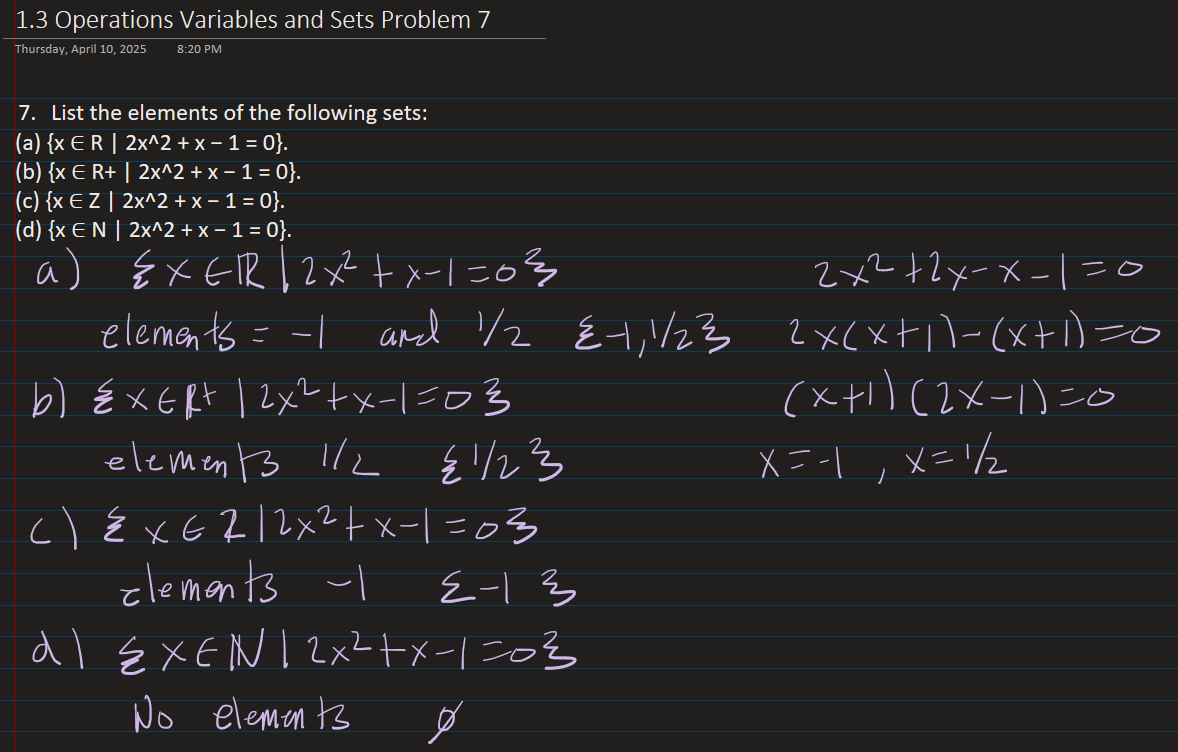
\includegraphics[width=0.8\textwidth]{images/1.2/24.PNG}
\end{figure}

\textbf{Problem 9:}
\begin{figure}[H]
    \centering
    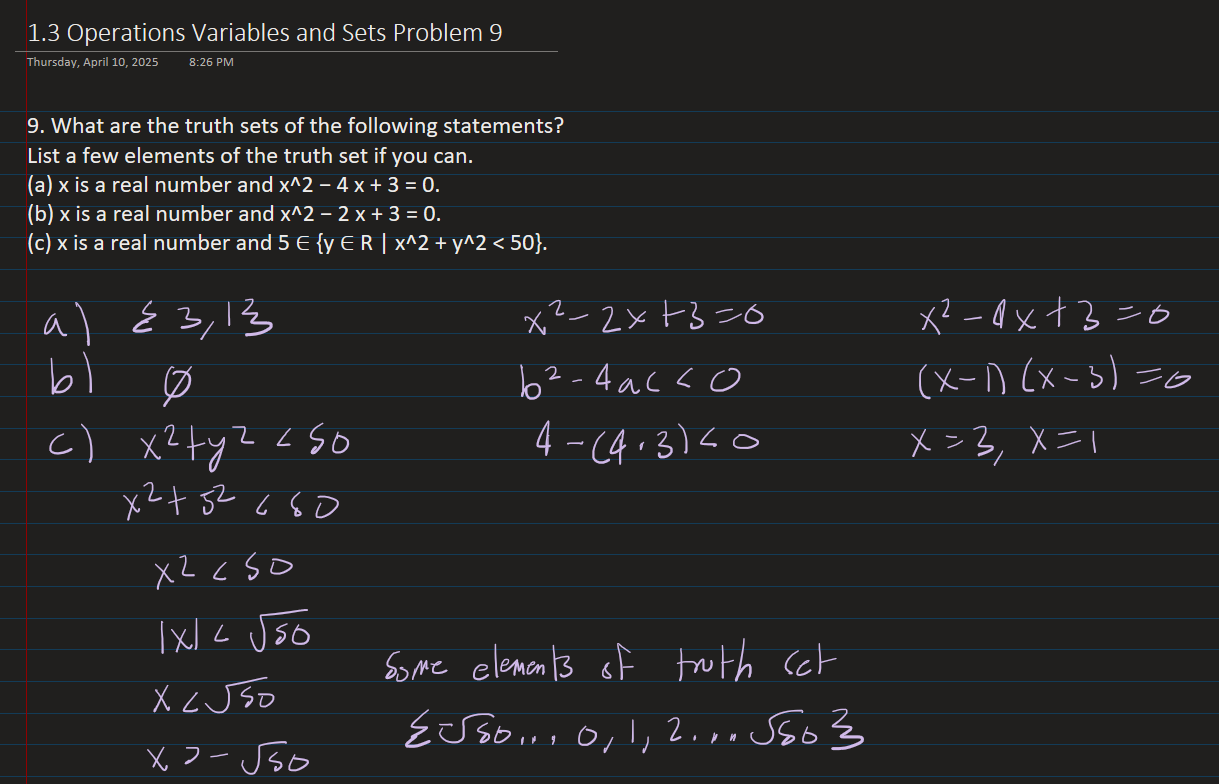
\includegraphics[width=0.8\textwidth]{images/1.2/25.PNG}
\end{figure}

\subsection{Operations On Sets}

\begin{tcolorbox}[title=Problem 2, breakable]
Let $A = \{\text{United States}, \text{Germany}, \text{China}, \text{Australia}\}$,\\
$B = \{\text{Germany}, \text{France}, \text{India}, \text{Brazil}\}$, and\\
$C = \{x \mid x \text{ is a country in Europe}\}$.\\

List the elements of the following sets. Are any of the sets below disjoint from any 
of the others? Are any of the sets below subsets of any others?
\end{tcolorbox}

\begin{tcolorbox}[title=Problem 2 (a), breakable]
$A \cup B$ 
\end{tcolorbox}

\textbf{Solution:}
\begin{align*}
A \cup B = \text{\{United States, Germany, China, Australia, France, India, Brazil\}} & \\
\end{align*}

\begin{tcolorbox}[title=Problem 2 (b), breakable]
$A \cap B \setminus C$
\end{tcolorbox}

\textbf{Solution:}
\begin{align*}
A \cap B = \text{\{Germany\}} & \\
A \cap B \setminus C = \emptyset  & \\
\end{align*}

\begin{tcolorbox}[title=Problem 2 (c), breakable]
$A \cap B \setminus A$
\end{tcolorbox}

\textbf{Solution:}
\begin{align*}
A \cap B = \text{\{Germany\}} & \\
A \cap B \setminus A = \emptyset && \\
(A \cap B \setminus C) \text{ and } (A \cap B \setminus A) \text{ are subsets of each other and } A \cup B& \\
(A \cap B \setminus C) \text{ and } (A \cap B \setminus A) \text{ are disjoint from each other and from } A \cup B& \\
\end{align*}

\textbf{Problem 3:}
\begin{figure}[H]
    \centering
    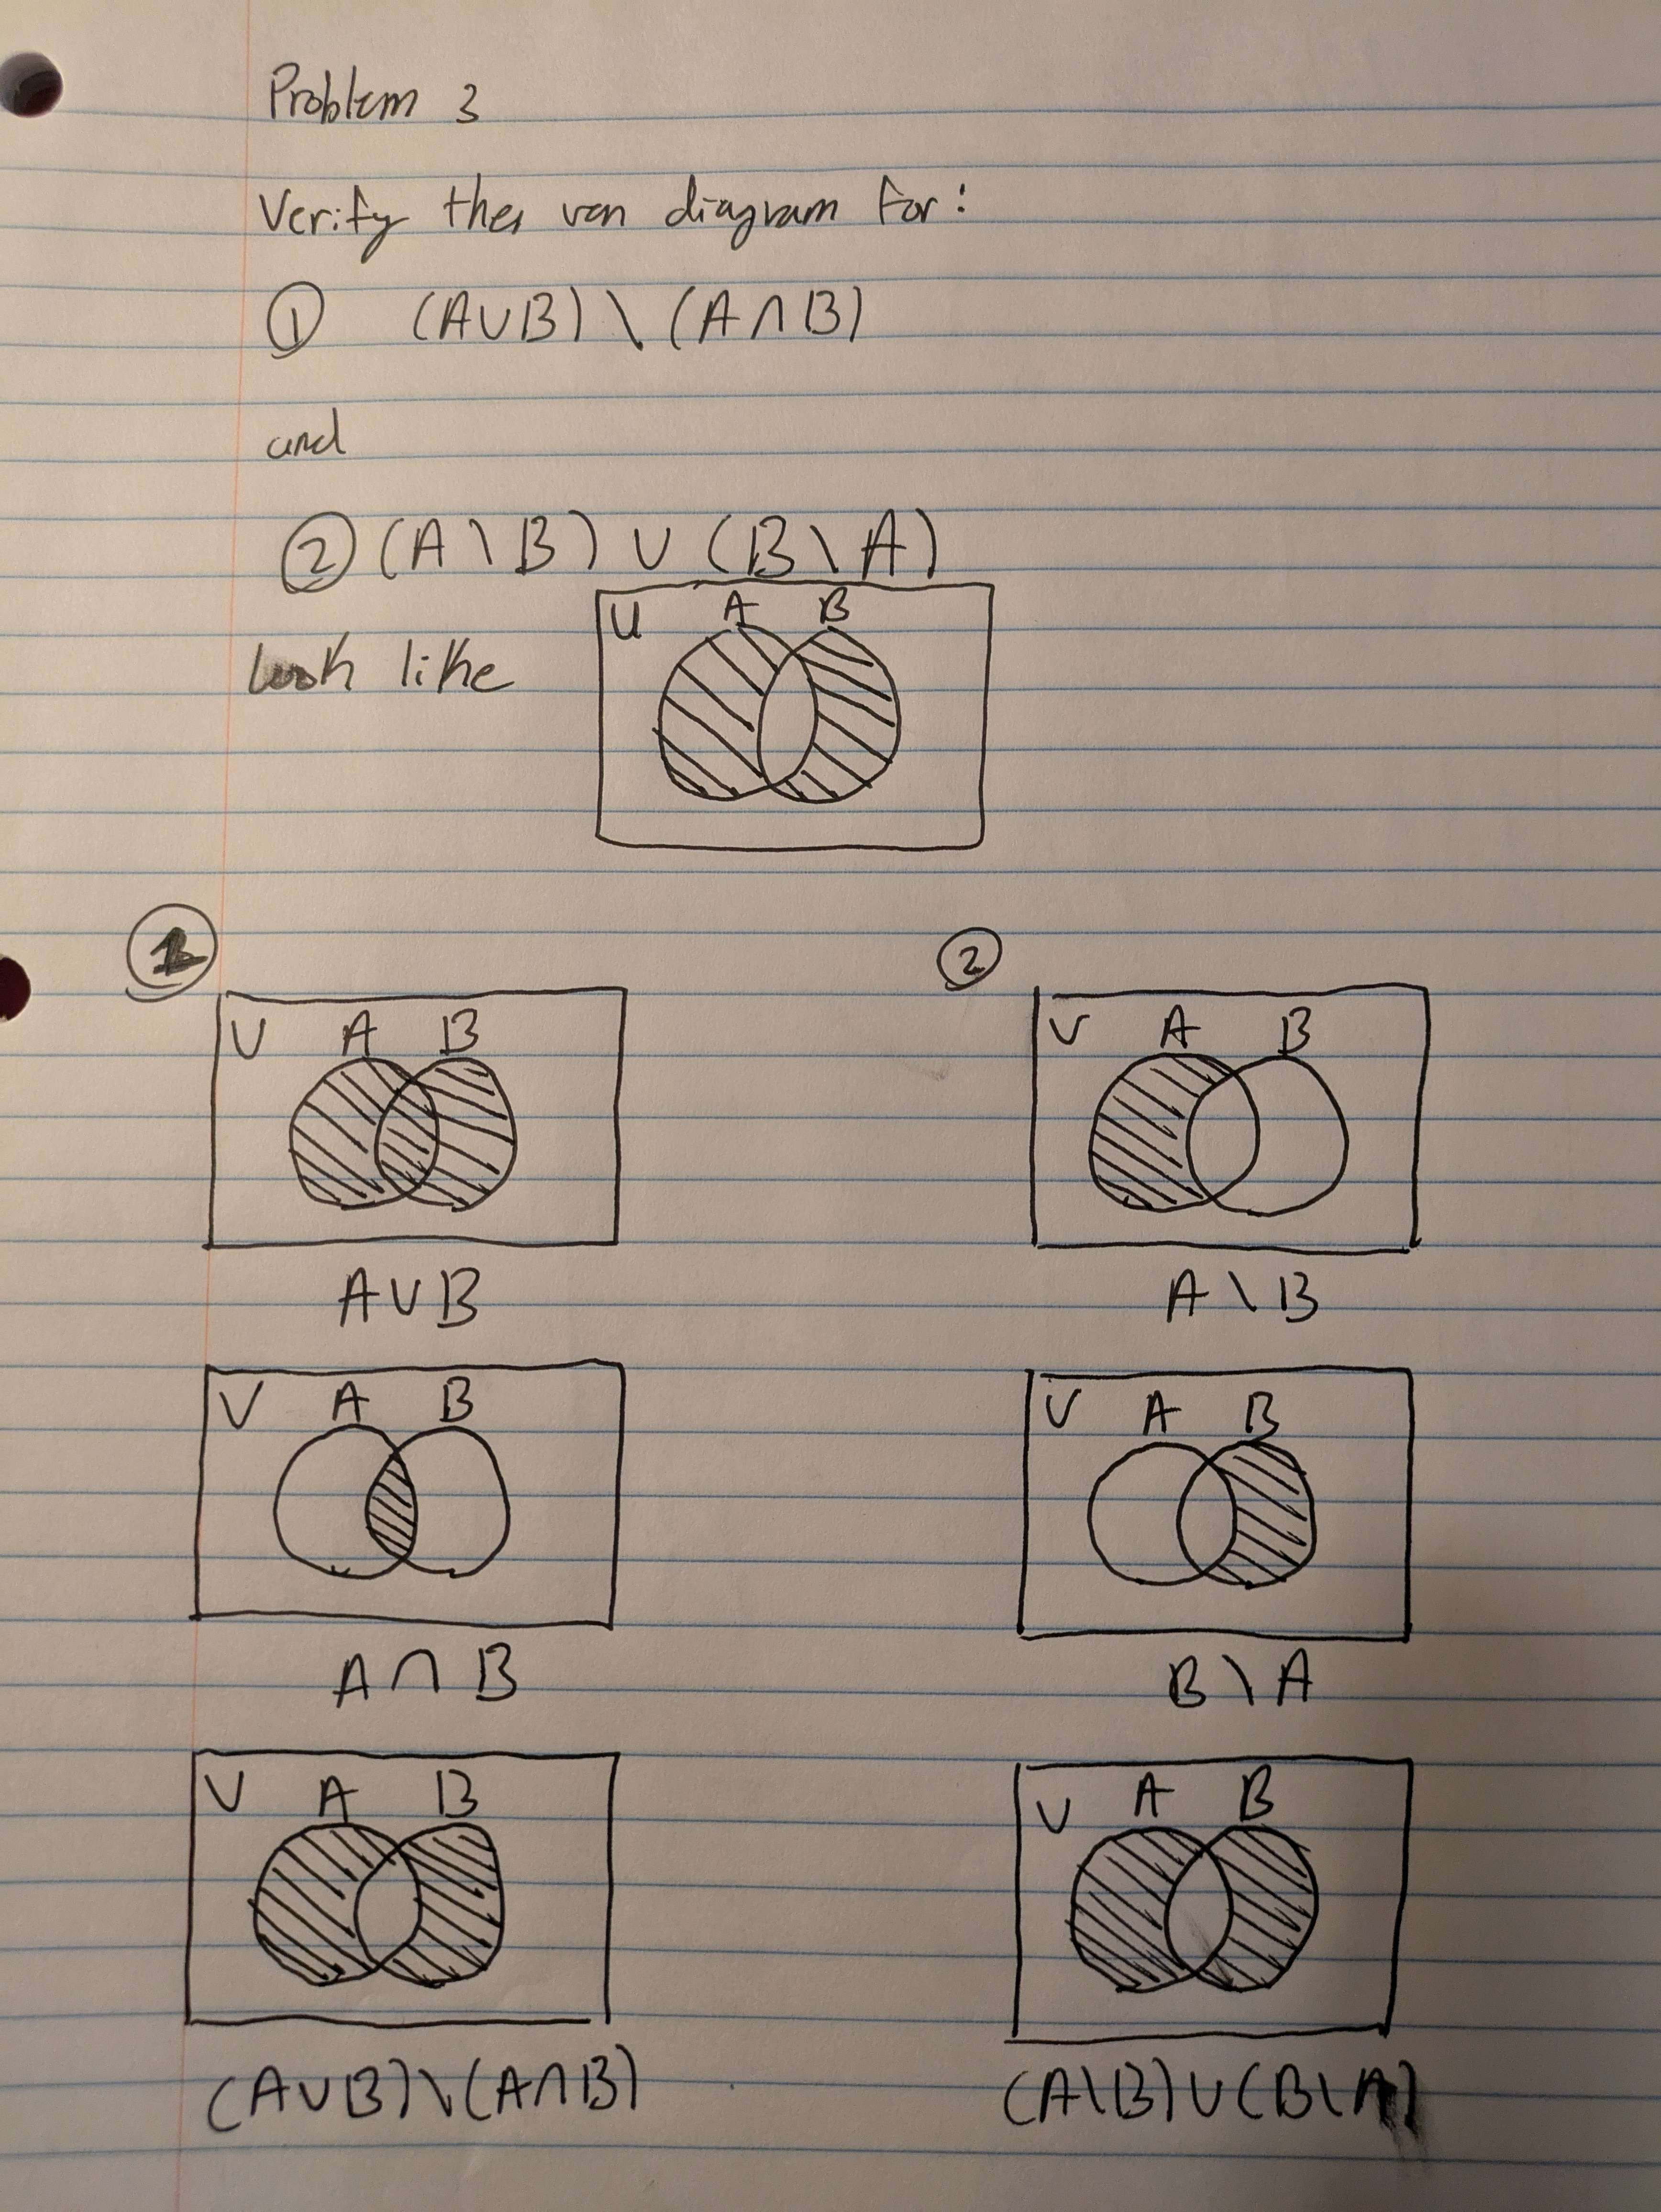
\includegraphics[width=0.8\textwidth]{images/1.2/1.jpg}
\end{figure}

\textbf{Problem 4(a):}
\begin{figure}[H]
    \centering
    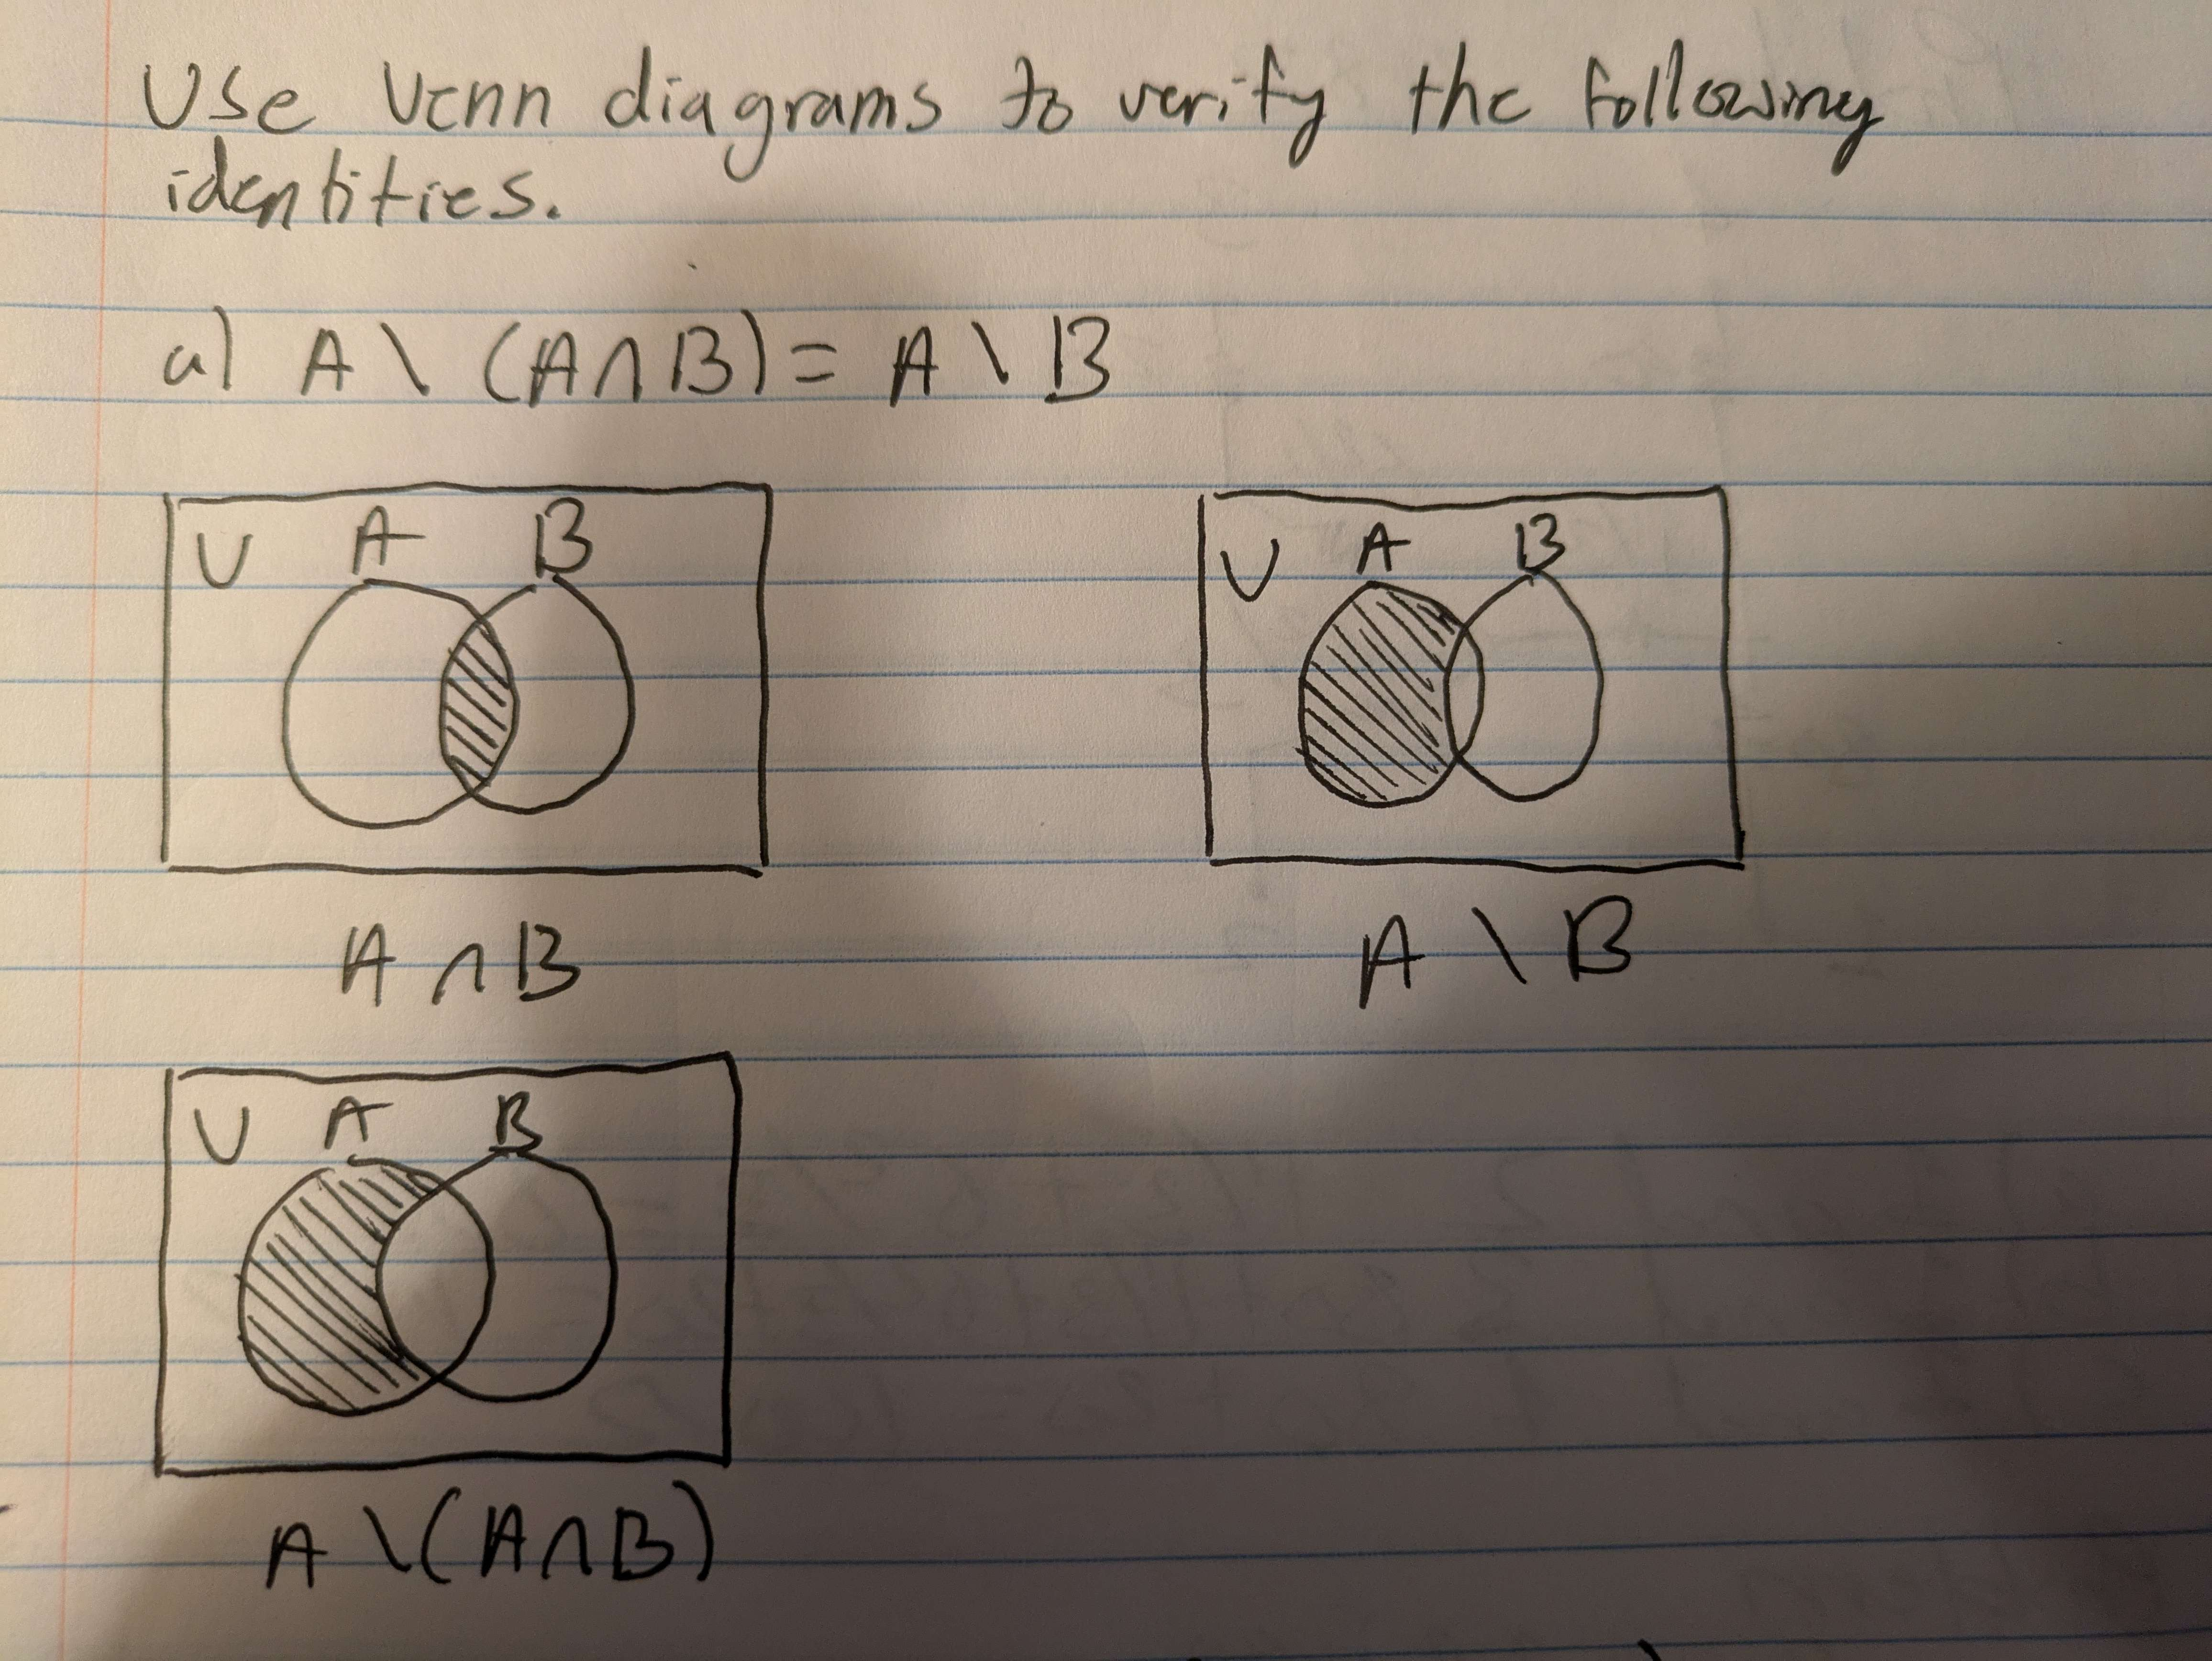
\includegraphics[width=0.8\textwidth]{images/1.2/2.jpg}
\end{figure}

\textbf{Problem 4(b):}
\begin{figure}[H]
    \centering
    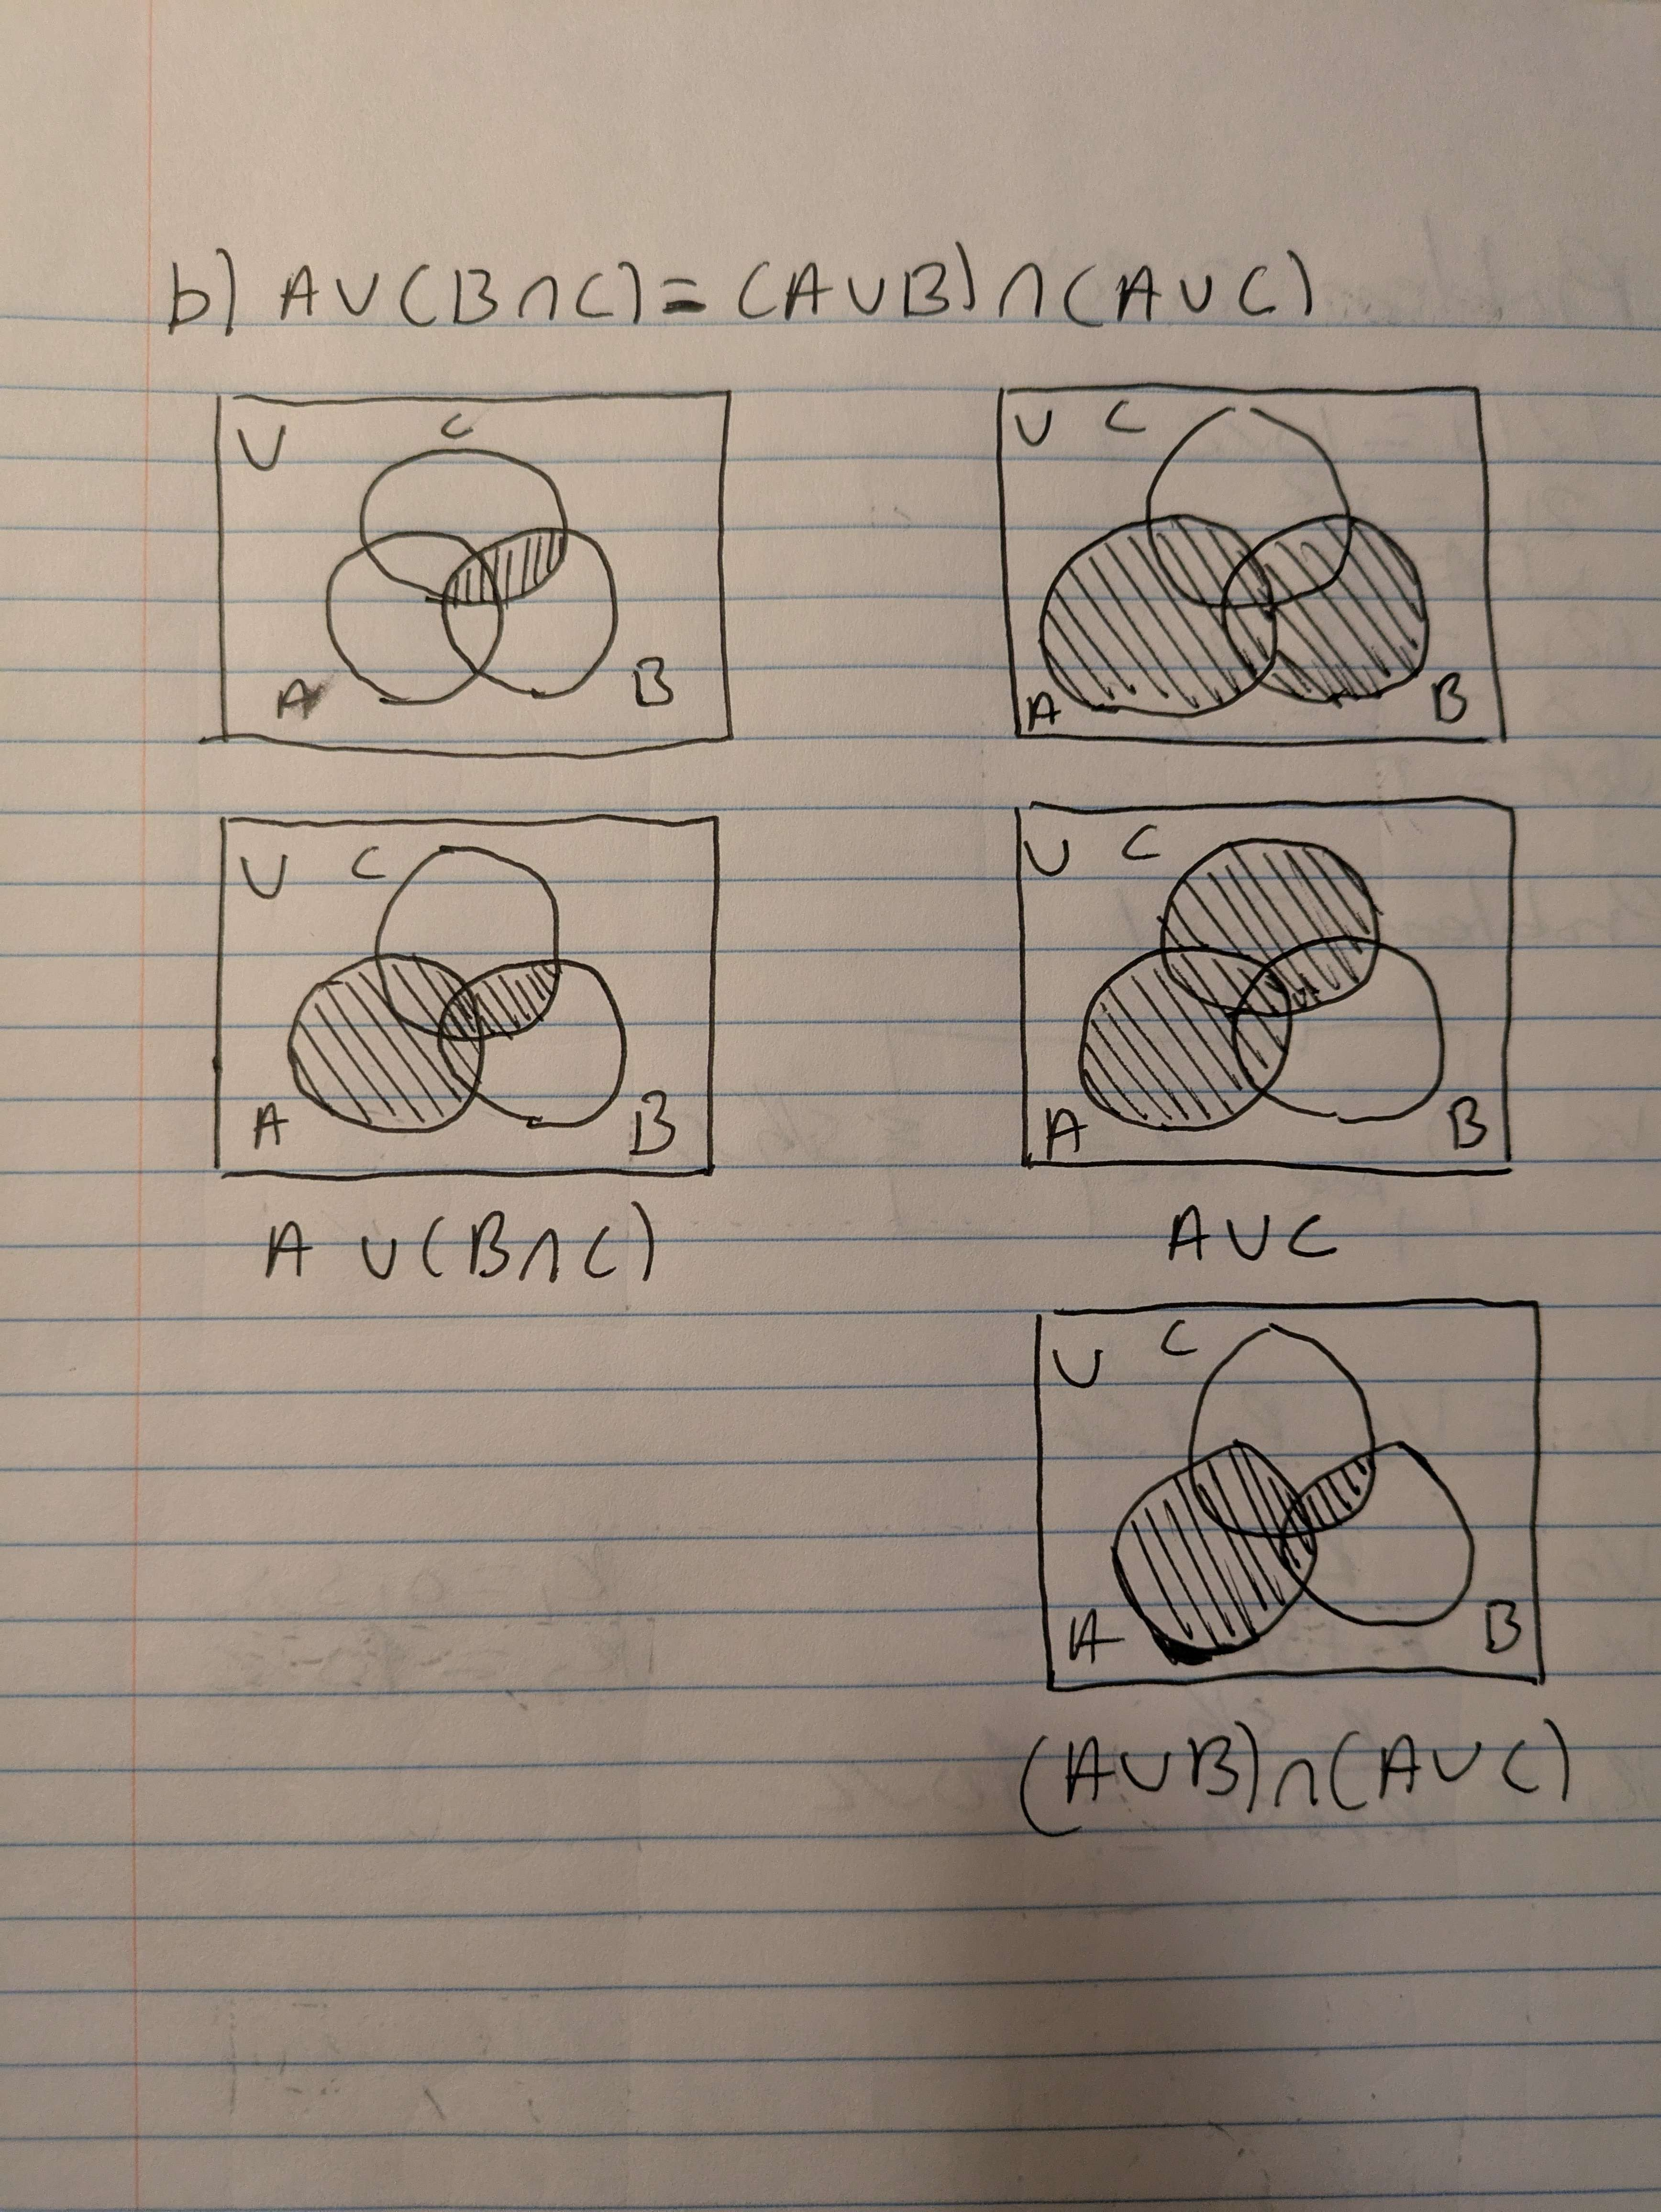
\includegraphics[width=0.8\textwidth]{images/1.2/3.jpg}
\end{figure}

\begin{tcolorbox}[title=Problem 5, breakable]
Verify the identities in exercise 4 by writing out (using
logical symbols) what it means for an object x to be an element
of each set and then using logical equivalences.

Excersize 4: 

(a) $A \setminus (A \cap B) = A \setminus B$ 

(b) $A \cup (B \cap C) = (A \cup B) \cap (A \cup C)$
\end{tcolorbox}

\textbf{Solution a:}
\begin{align*}
\text{Let } X &\equiv (x \in A) \\
\text{Let } Y &\equiv (x \in B) \\ \\
x \in A \setminus (A \cap B) &\equiv (x \in A) \wedge \neg(x \in A \wedge x \in B) & \\
&\equiv (x \in A) \wedge (x \not \in A \vee x \not \in B) & \\
&\equiv X \wedge (\neg X \vee \neg Y) & \\
&\equiv (X \wedge \neg X) \vee (X \wedge \neg Y) & \\
&\equiv X \wedge \neg Y & \\
&\equiv x \in A \wedge x \not \in B & \\
&\equiv x \in A \setminus B & \\
\end{align*}

\textbf{Solution b:}
\begin{align*}
\text{Let } X &\equiv (x \in A) \\
\text{Let } Y &\equiv (x \in B) \\
\text{Let } Z &\equiv (x \in C) \\ \\
x \in A \cup (B \cap C) &\equiv x \in A \vee x \in (B \cap C) &\quad \text{def. of union} & \\
&\equiv x \in A \vee x \in (x \in B \wedge x \in C) &\quad \text{def. of intersection} & \\
&\equiv X \vee (Y \wedge Z) &\quad \text{def. of intersection} & \\
&\equiv (X \vee Y) \wedge (X \vee Z) &\quad \text{} & \\
&\equiv (x \in A \vee x \in B) \wedge (x \in A \vee x \in C) &\quad \text{} & \\
&\equiv (x \in A \cup B) \wedge (x \in A \cup C) &\quad \text{def. of union} & \\
&\equiv x \in (A \cup B) \cap (A \cup C) &\quad \text{def. of intersection} & \\
\end{align*}

\textbf{Problem 6:}
\begin{figure}[H]
    \centering
    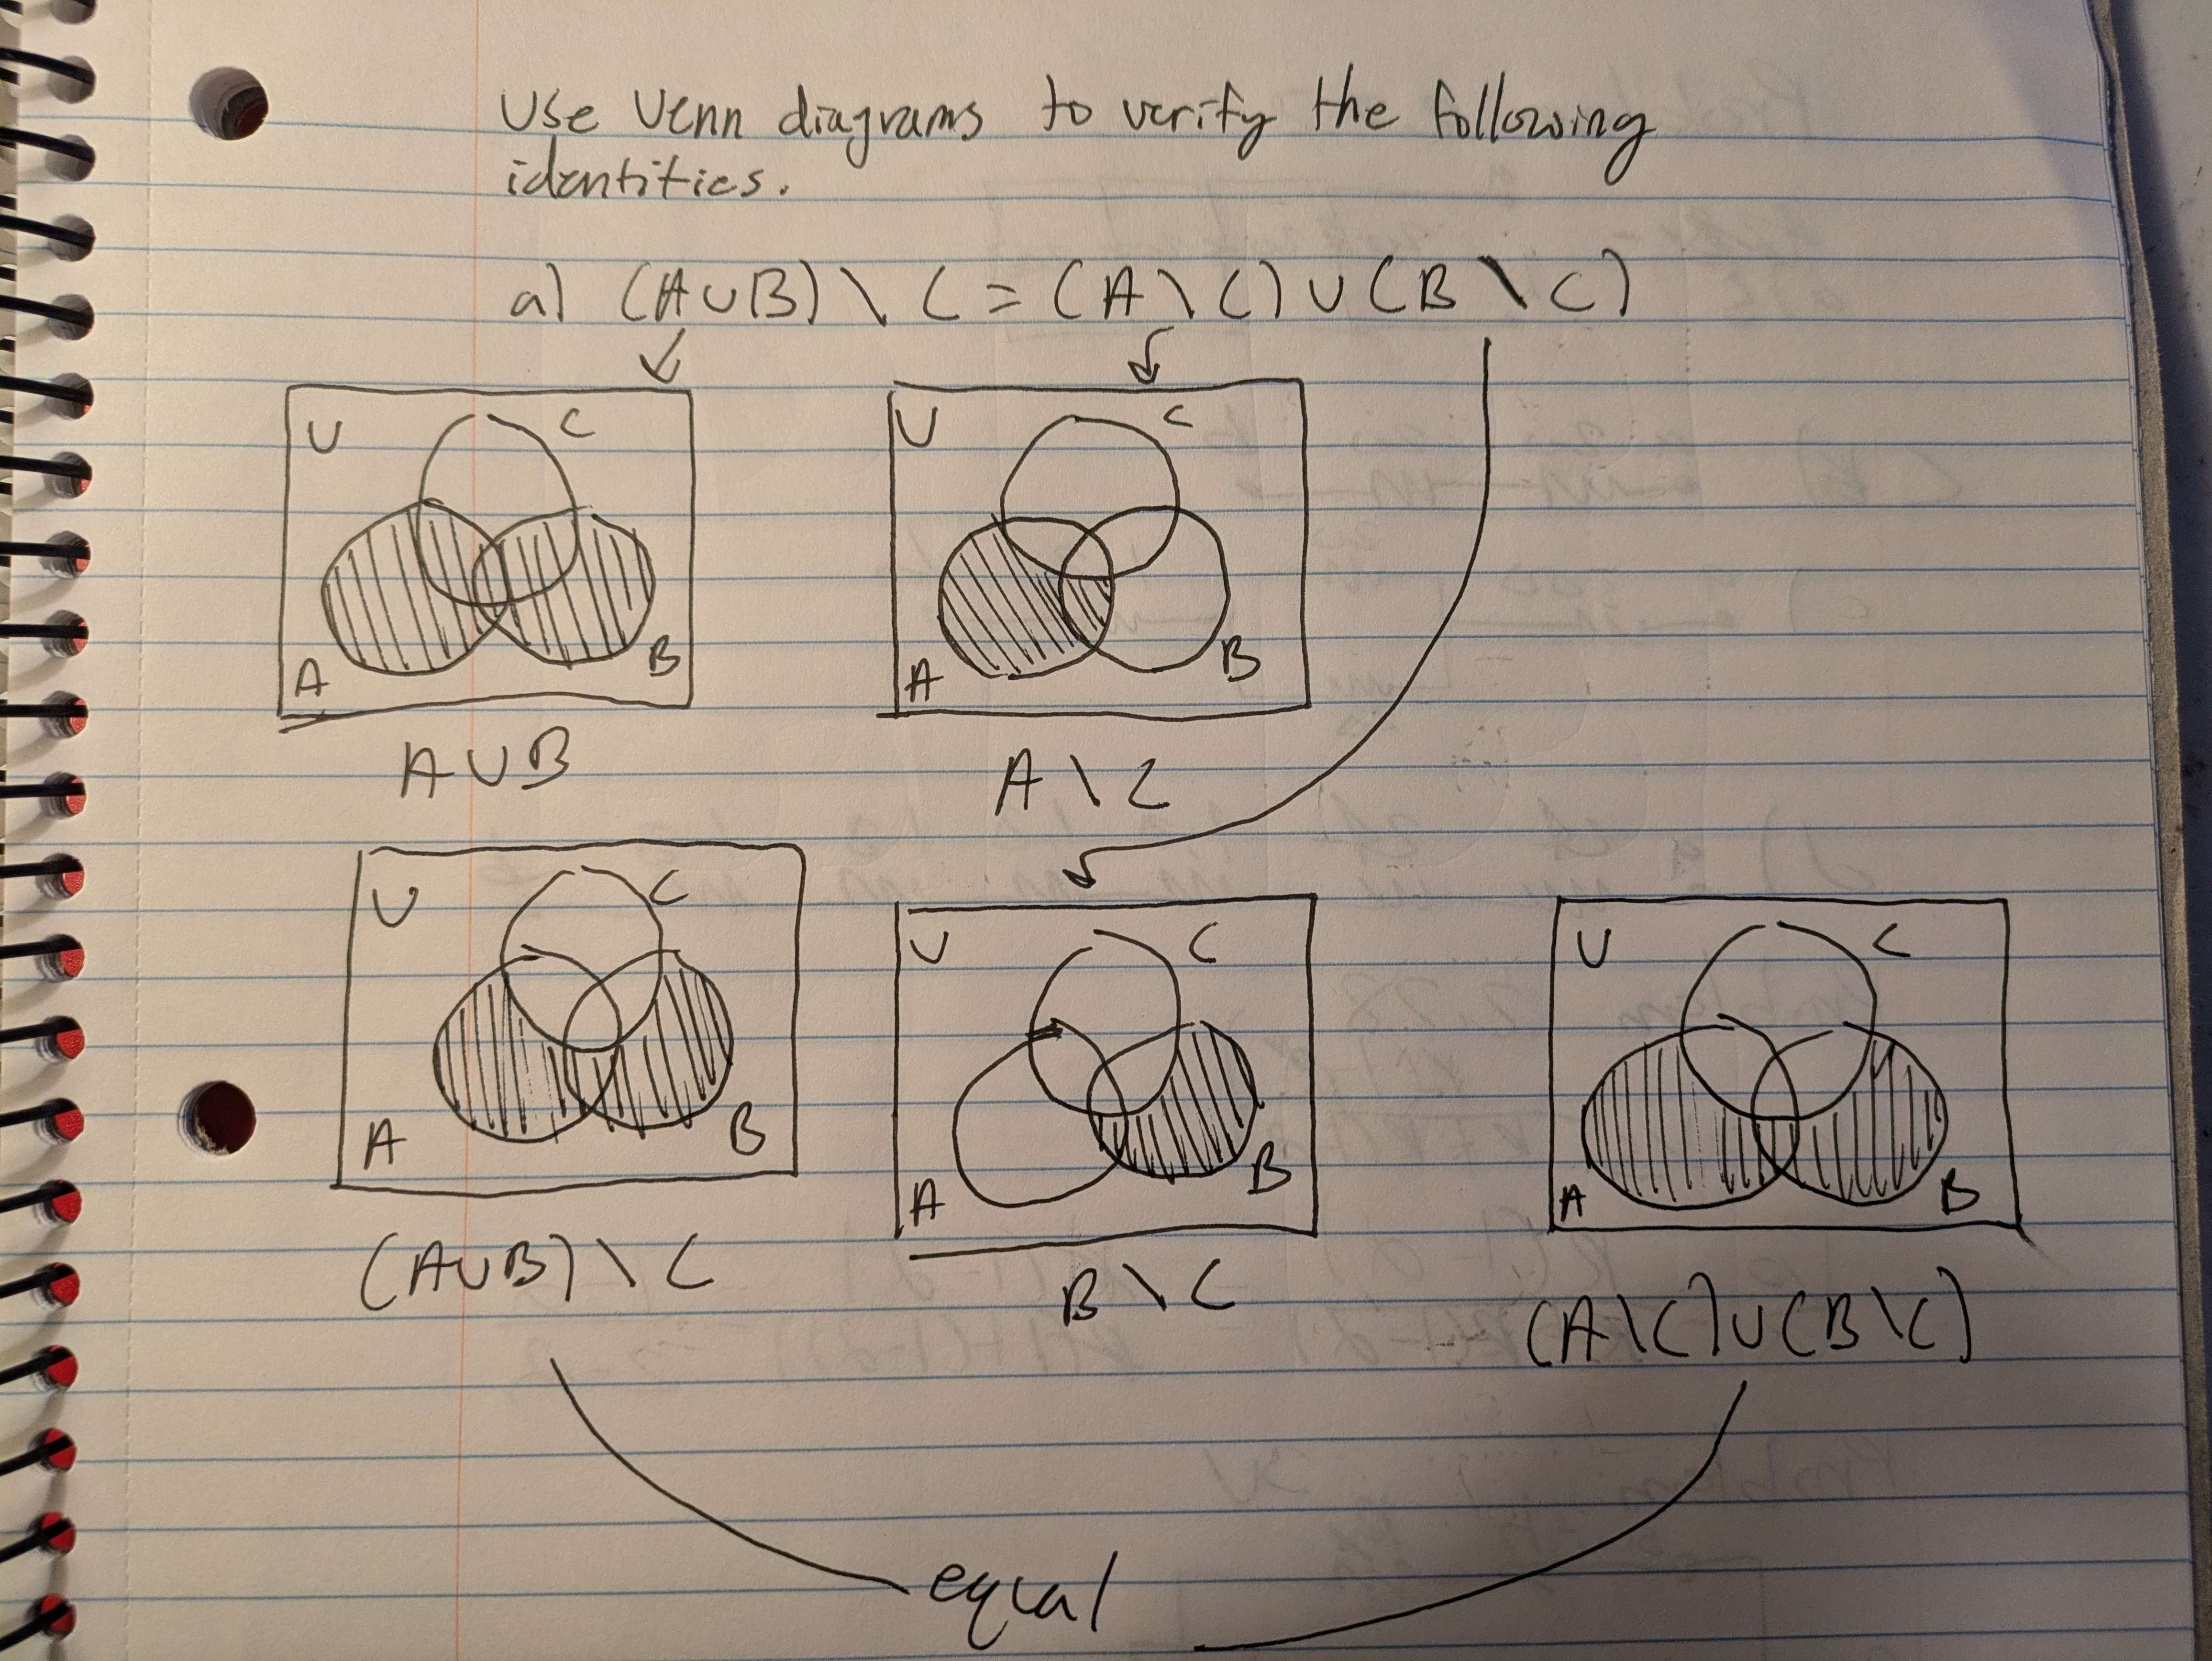
\includegraphics[width=0.8\textwidth]{images/1.2/4.jpg}
\end{figure}
\begin{figure}[H]
    \centering
    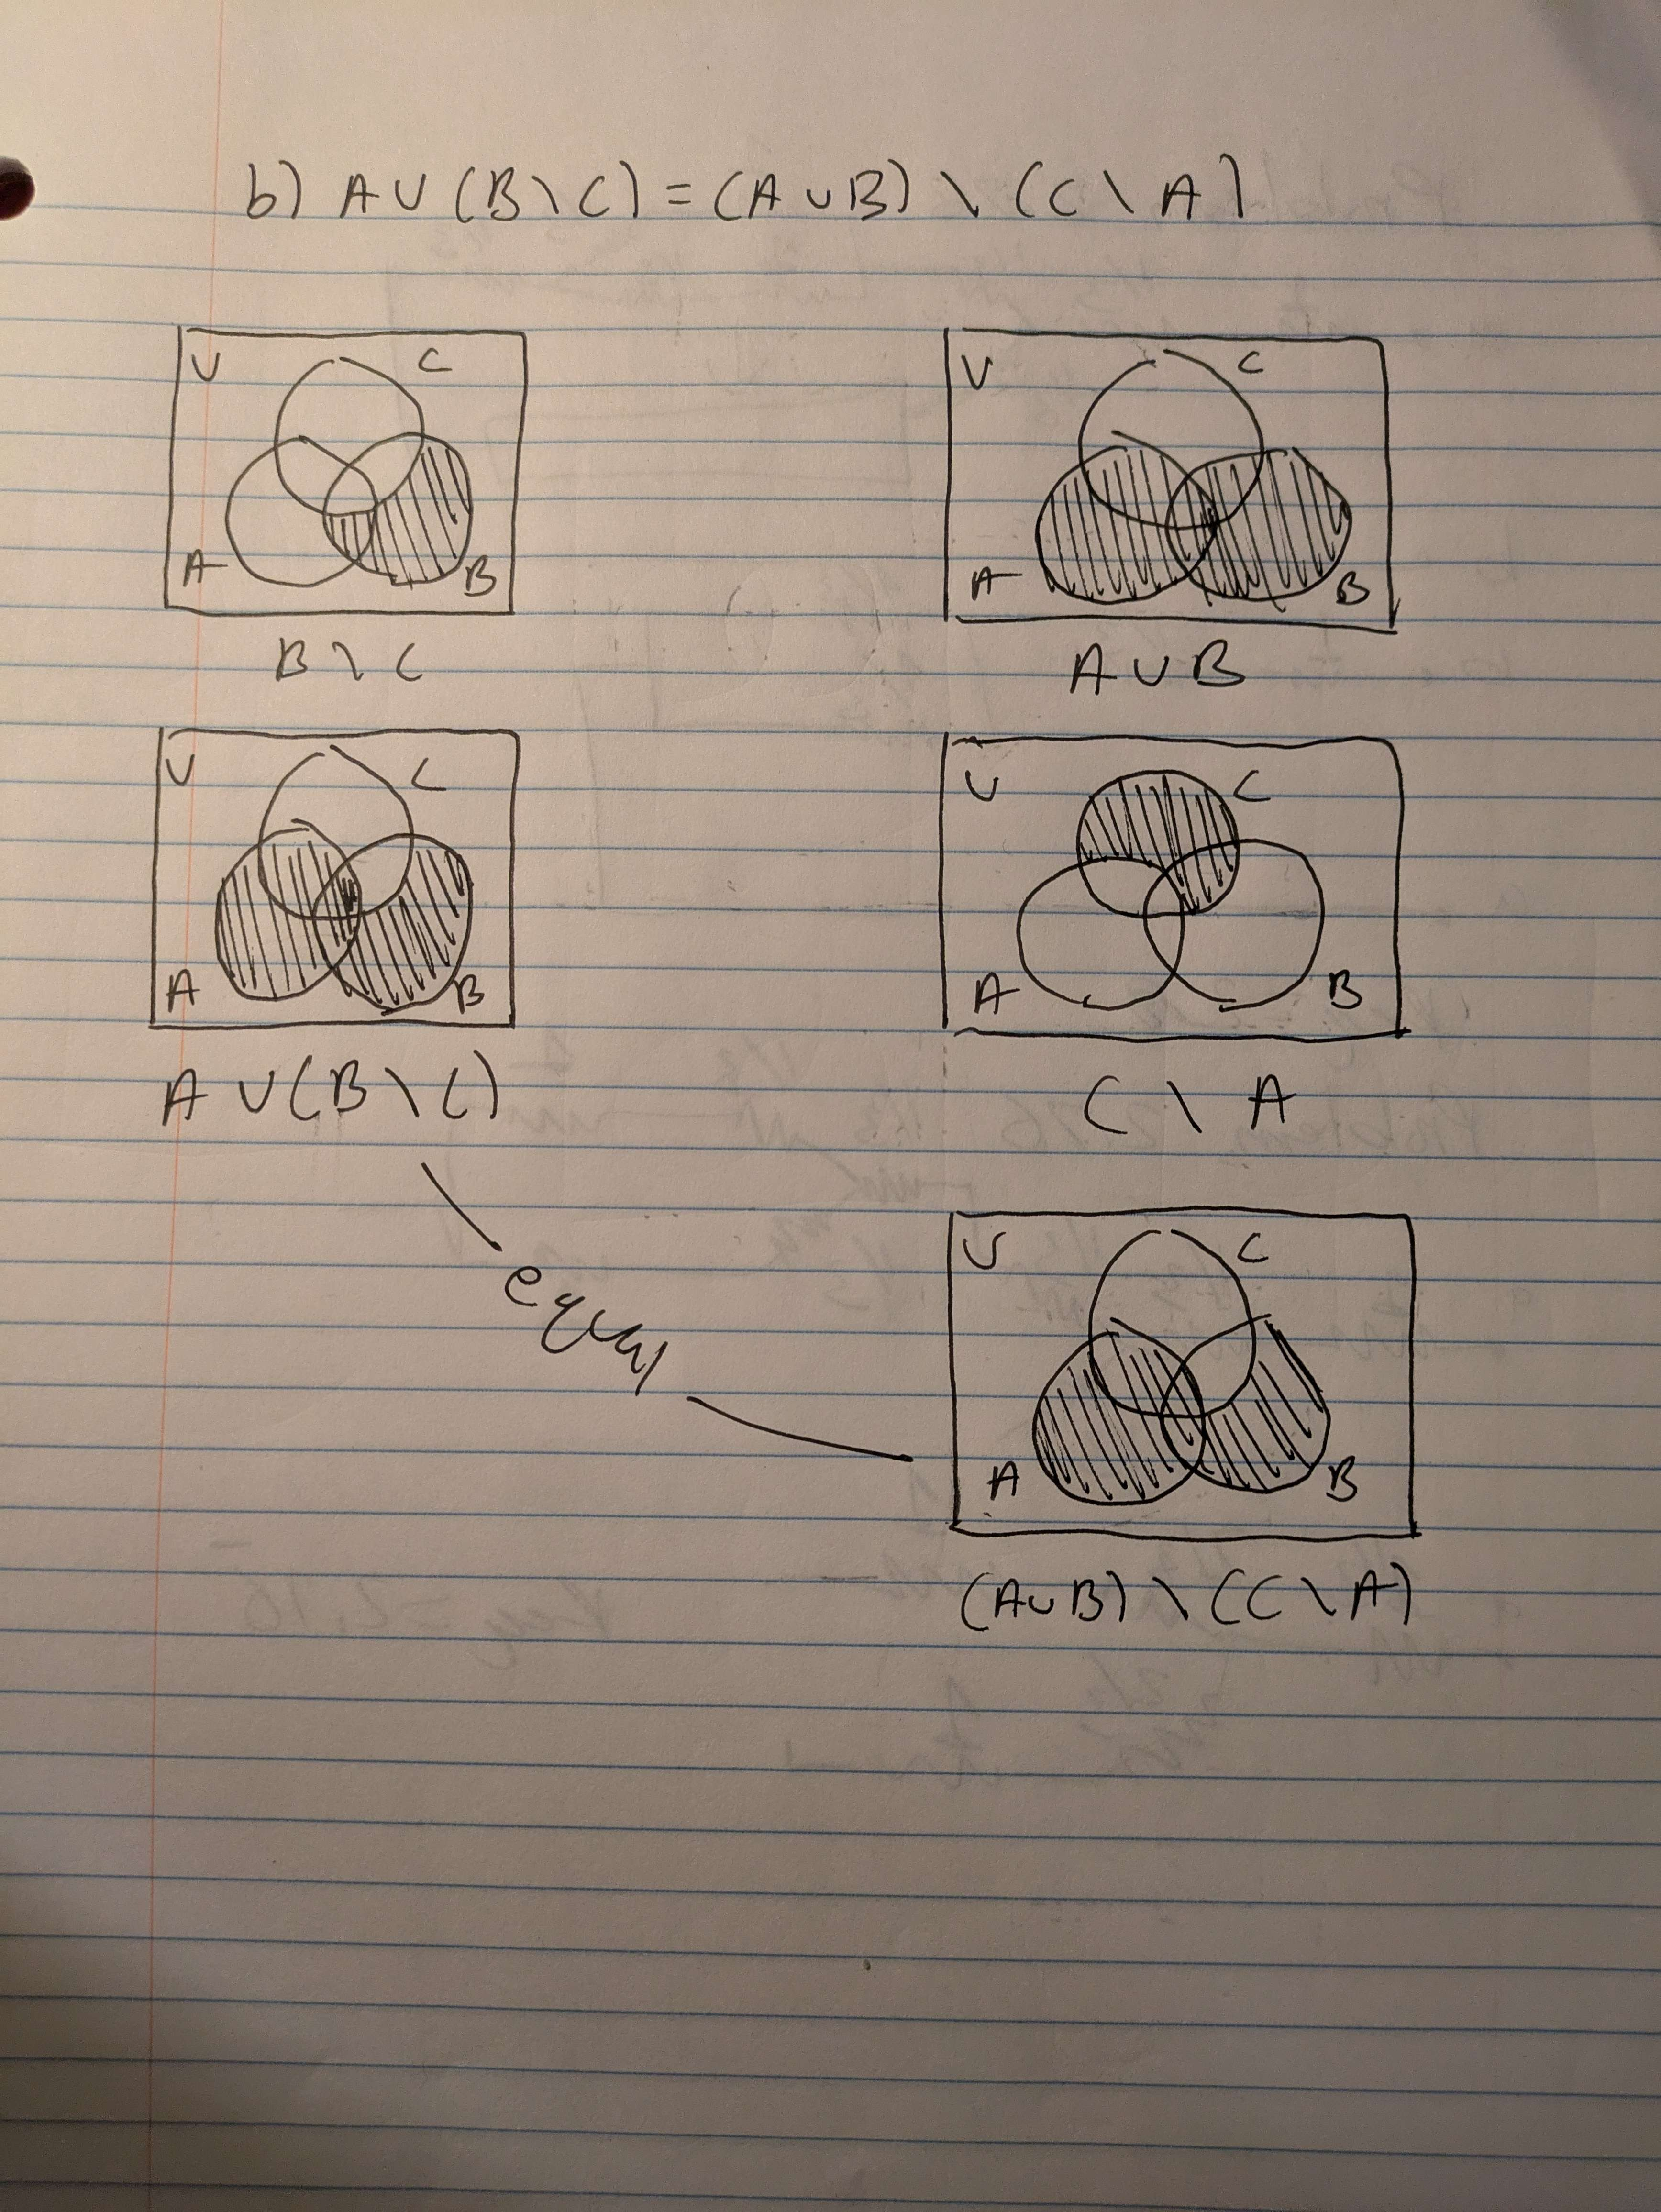
\includegraphics[width=0.8\textwidth]{images/1.2/5.jpg}
\end{figure}

\begin{tcolorbox}[title=Problem 7, breakable]
Verify the identities in excersize $6$ by writing out (using logical symbols) what 
it means for an object $x$ to be an element of each set then using logical
equivalences. \\
(a) $(A \cup B) \setminus C \equiv (A \setminus C) \cup (B \setminus C)$ \\
(b) $A \cup (B \setminus C) \equiv (A \cup B) \setminus (C \setminus A)$
\end{tcolorbox}

\textbf{Solution a:}
\begin{align*}
\text{Let } X &\equiv (x \in A) & \\
\text{Let } Y &\equiv (x \in B) & \\
\text{Let } Z &\equiv (x \in C) & \\& \\
x \in (A \cup B) \setminus C &\equiv x \in (A \cup B) \wedge x \not \in C  &\quad \text{def. of set difference} & \\
&\equiv (x \in A \vee x \in B) \wedge x \not \in C  &\quad \text{def. of union} & \\
&\equiv (X \vee Y) \wedge \neg Z  &\quad \text{} & \\
&\equiv (X \wedge \neg Z) \vee (Y \wedge \neg Z)  &\quad \text{distributive} & \\
&\equiv (x \in A \wedge x \not \in C) \vee (x \in B \wedge x \not \in C)  &\quad \text{} & \\
&\equiv (x \in A \setminus C) \vee (x \in B \setminus C) &\quad \text{def. of set difference} & \\
&\equiv x \in (A \setminus C) \cup (B \setminus C) &\quad \text{def. of union} & \\
\end{align*}

\textbf{Solution b:}
\begin{align*}
\text{Let } X &\equiv (x \in A) & \\
\text{Let } Y &\equiv (x \in B) & \\
\text{Let } Z &\equiv (x \in C) & \\ & \\
x \in A \cup (B \setminus C) &\equiv x \in A \vee x \in (B \setminus C) &\quad \text{def. of union} & \\
&\equiv x \in A \vee (x \in B \wedge x \not \in C) & \quad \text {def. of set difference} & \\
&\equiv X \vee (Y \wedge \neg Z) & & \\
&\equiv (X \vee Y) \wedge (X \vee \neg Z) & \quad \text{distributive} & \\
&\equiv (X \vee Y) \wedge \neg (\neg X \wedge Z)  & \quad \text{demorgans} & \\
&\equiv (X \vee Y) \wedge \neg (Z \wedge \neg X) & \quad \text{commutative} & \\
&\equiv (x \in A \vee x \in B) \wedge \neg (x \in C \wedge x \not \in A) & \quad \text{} & \\
&\equiv x \in (A \cup B) \wedge \neg (x \in C \wedge x \not \in A) & \quad \text{def. of union} & \\
&\equiv x \in (A \cup B) \wedge \neg ( x \in (C \setminus A)) & \quad \text{def. of set difference} & \\
&\equiv x \in (A \cup B) \setminus (C \setminus A) & \quad \text{def. of set difference} & \\
\end{align*}

\textbf{Problem 8:}
\begin{figure}[H]
    \centering
    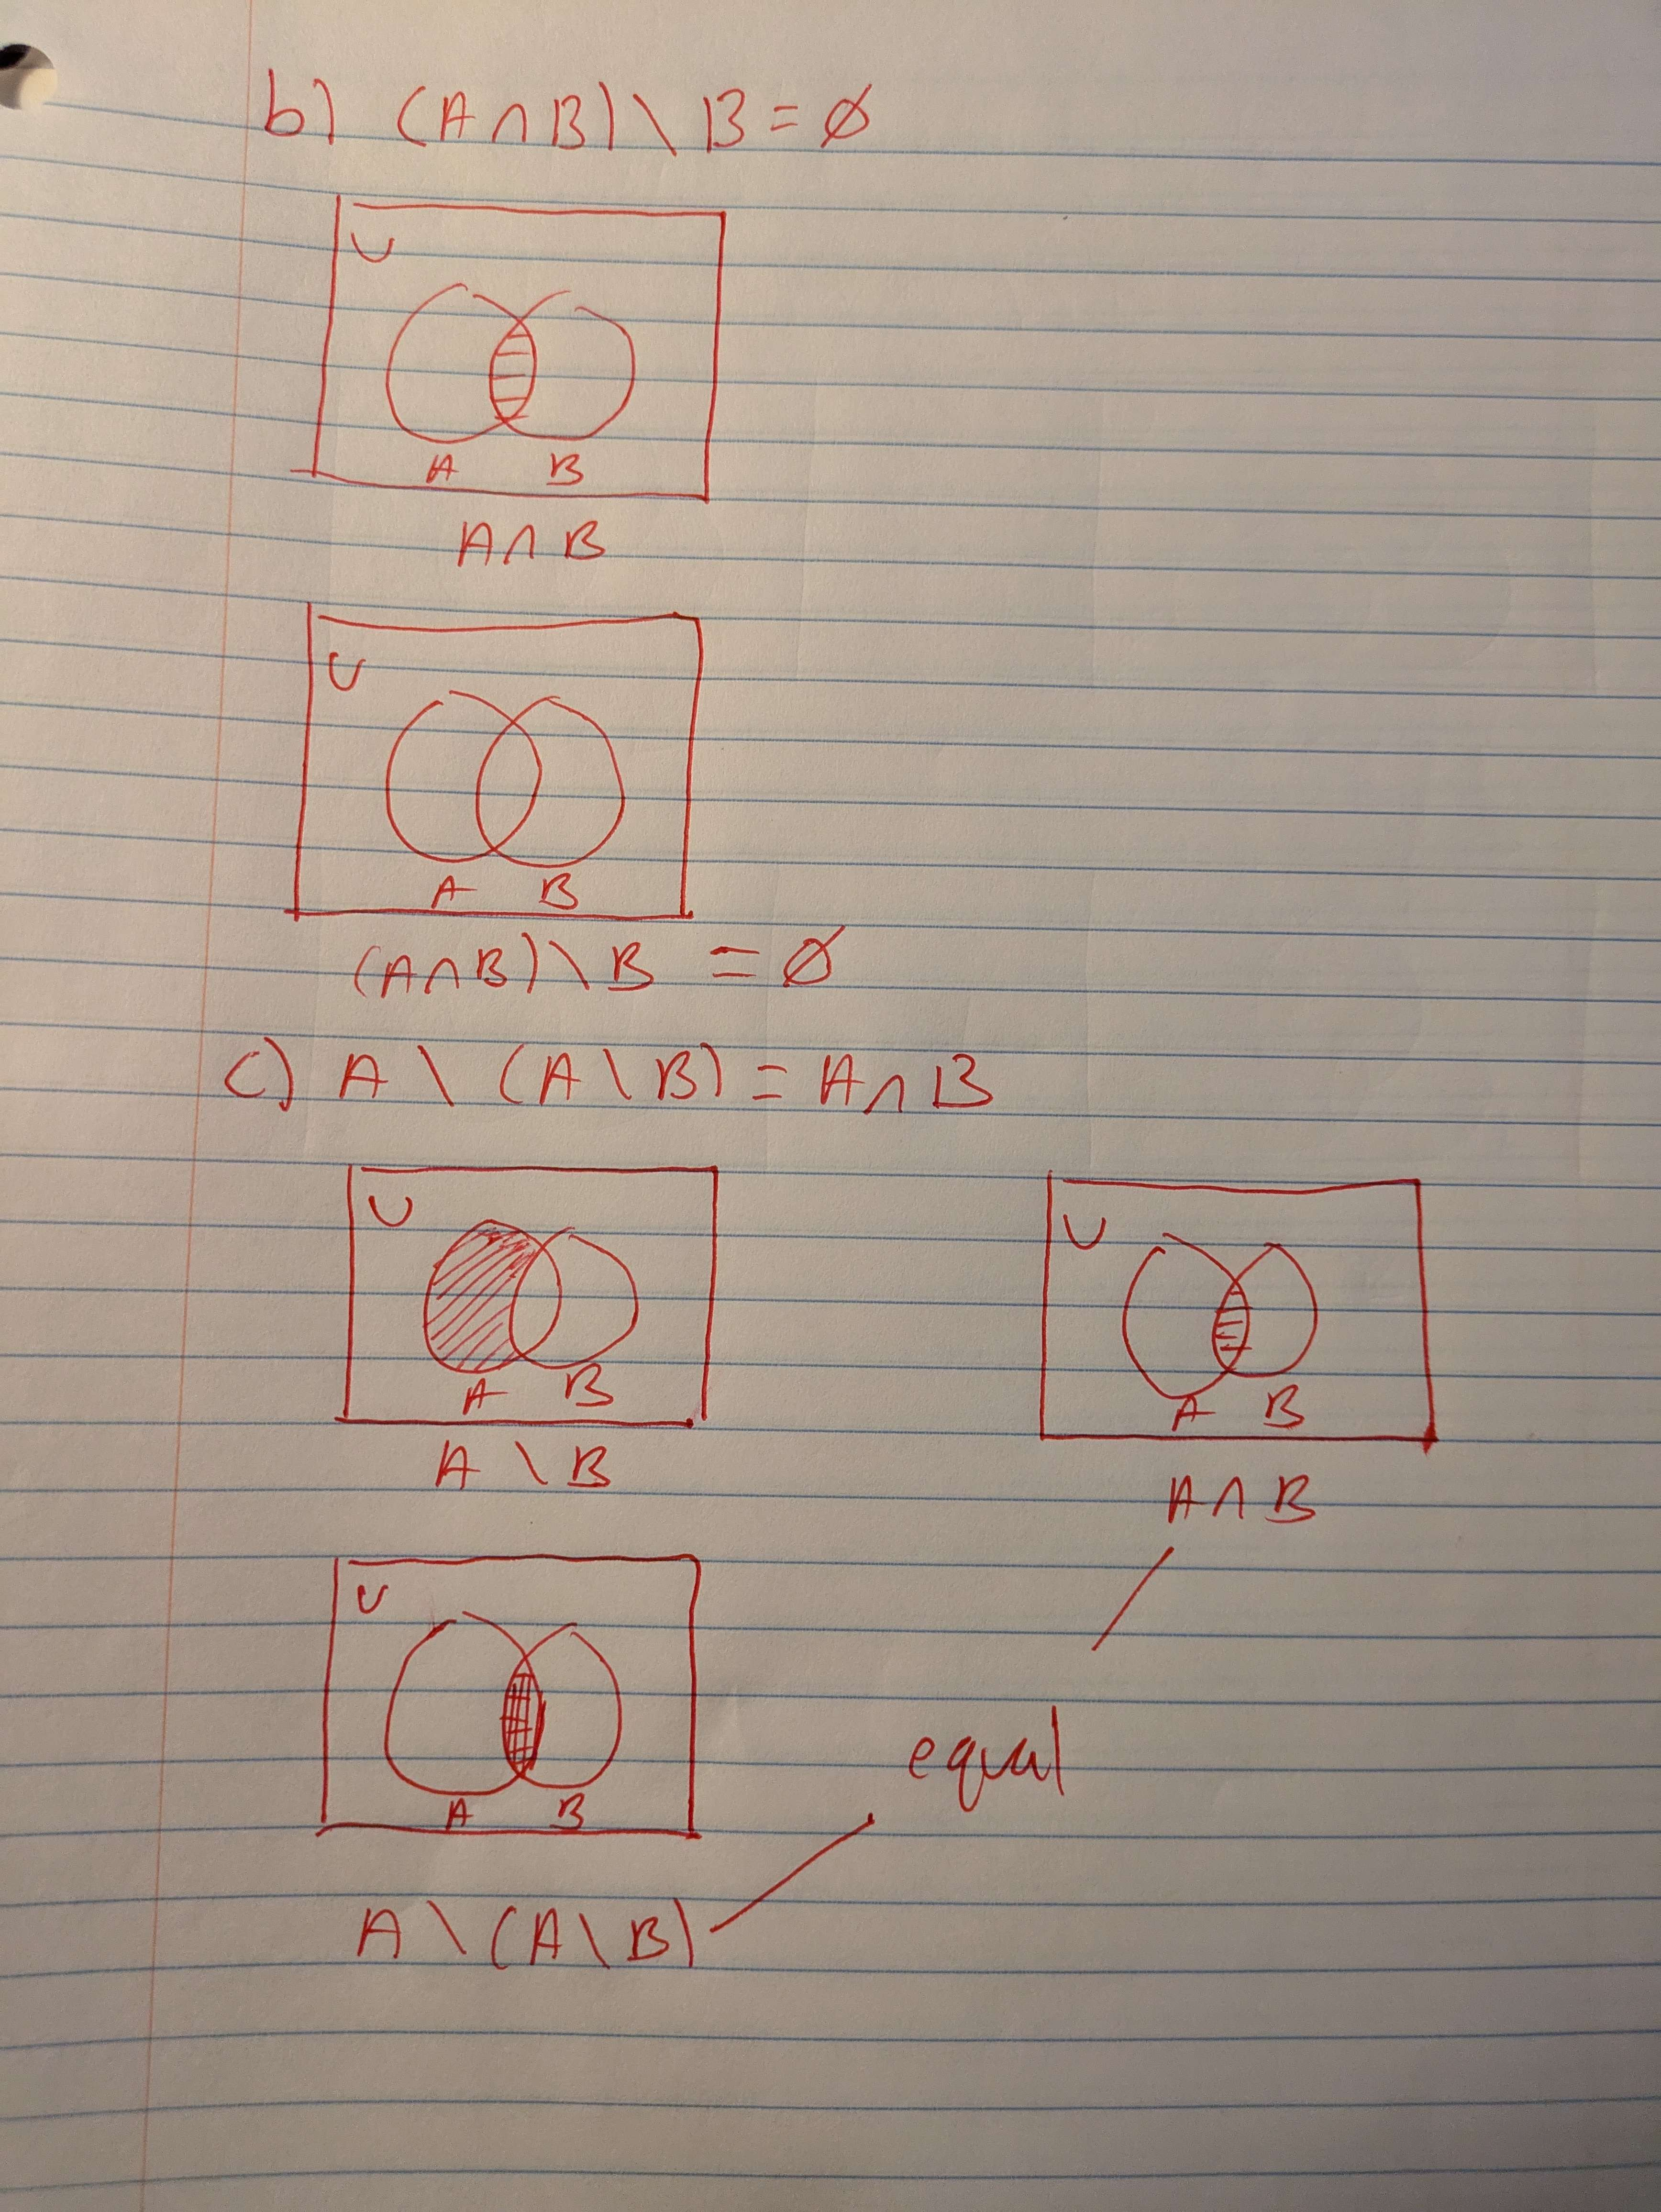
\includegraphics[width=0.8\textwidth]{images/1.2/6.jpg}
\end{figure}
\begin{figure}[H]
    \centering
    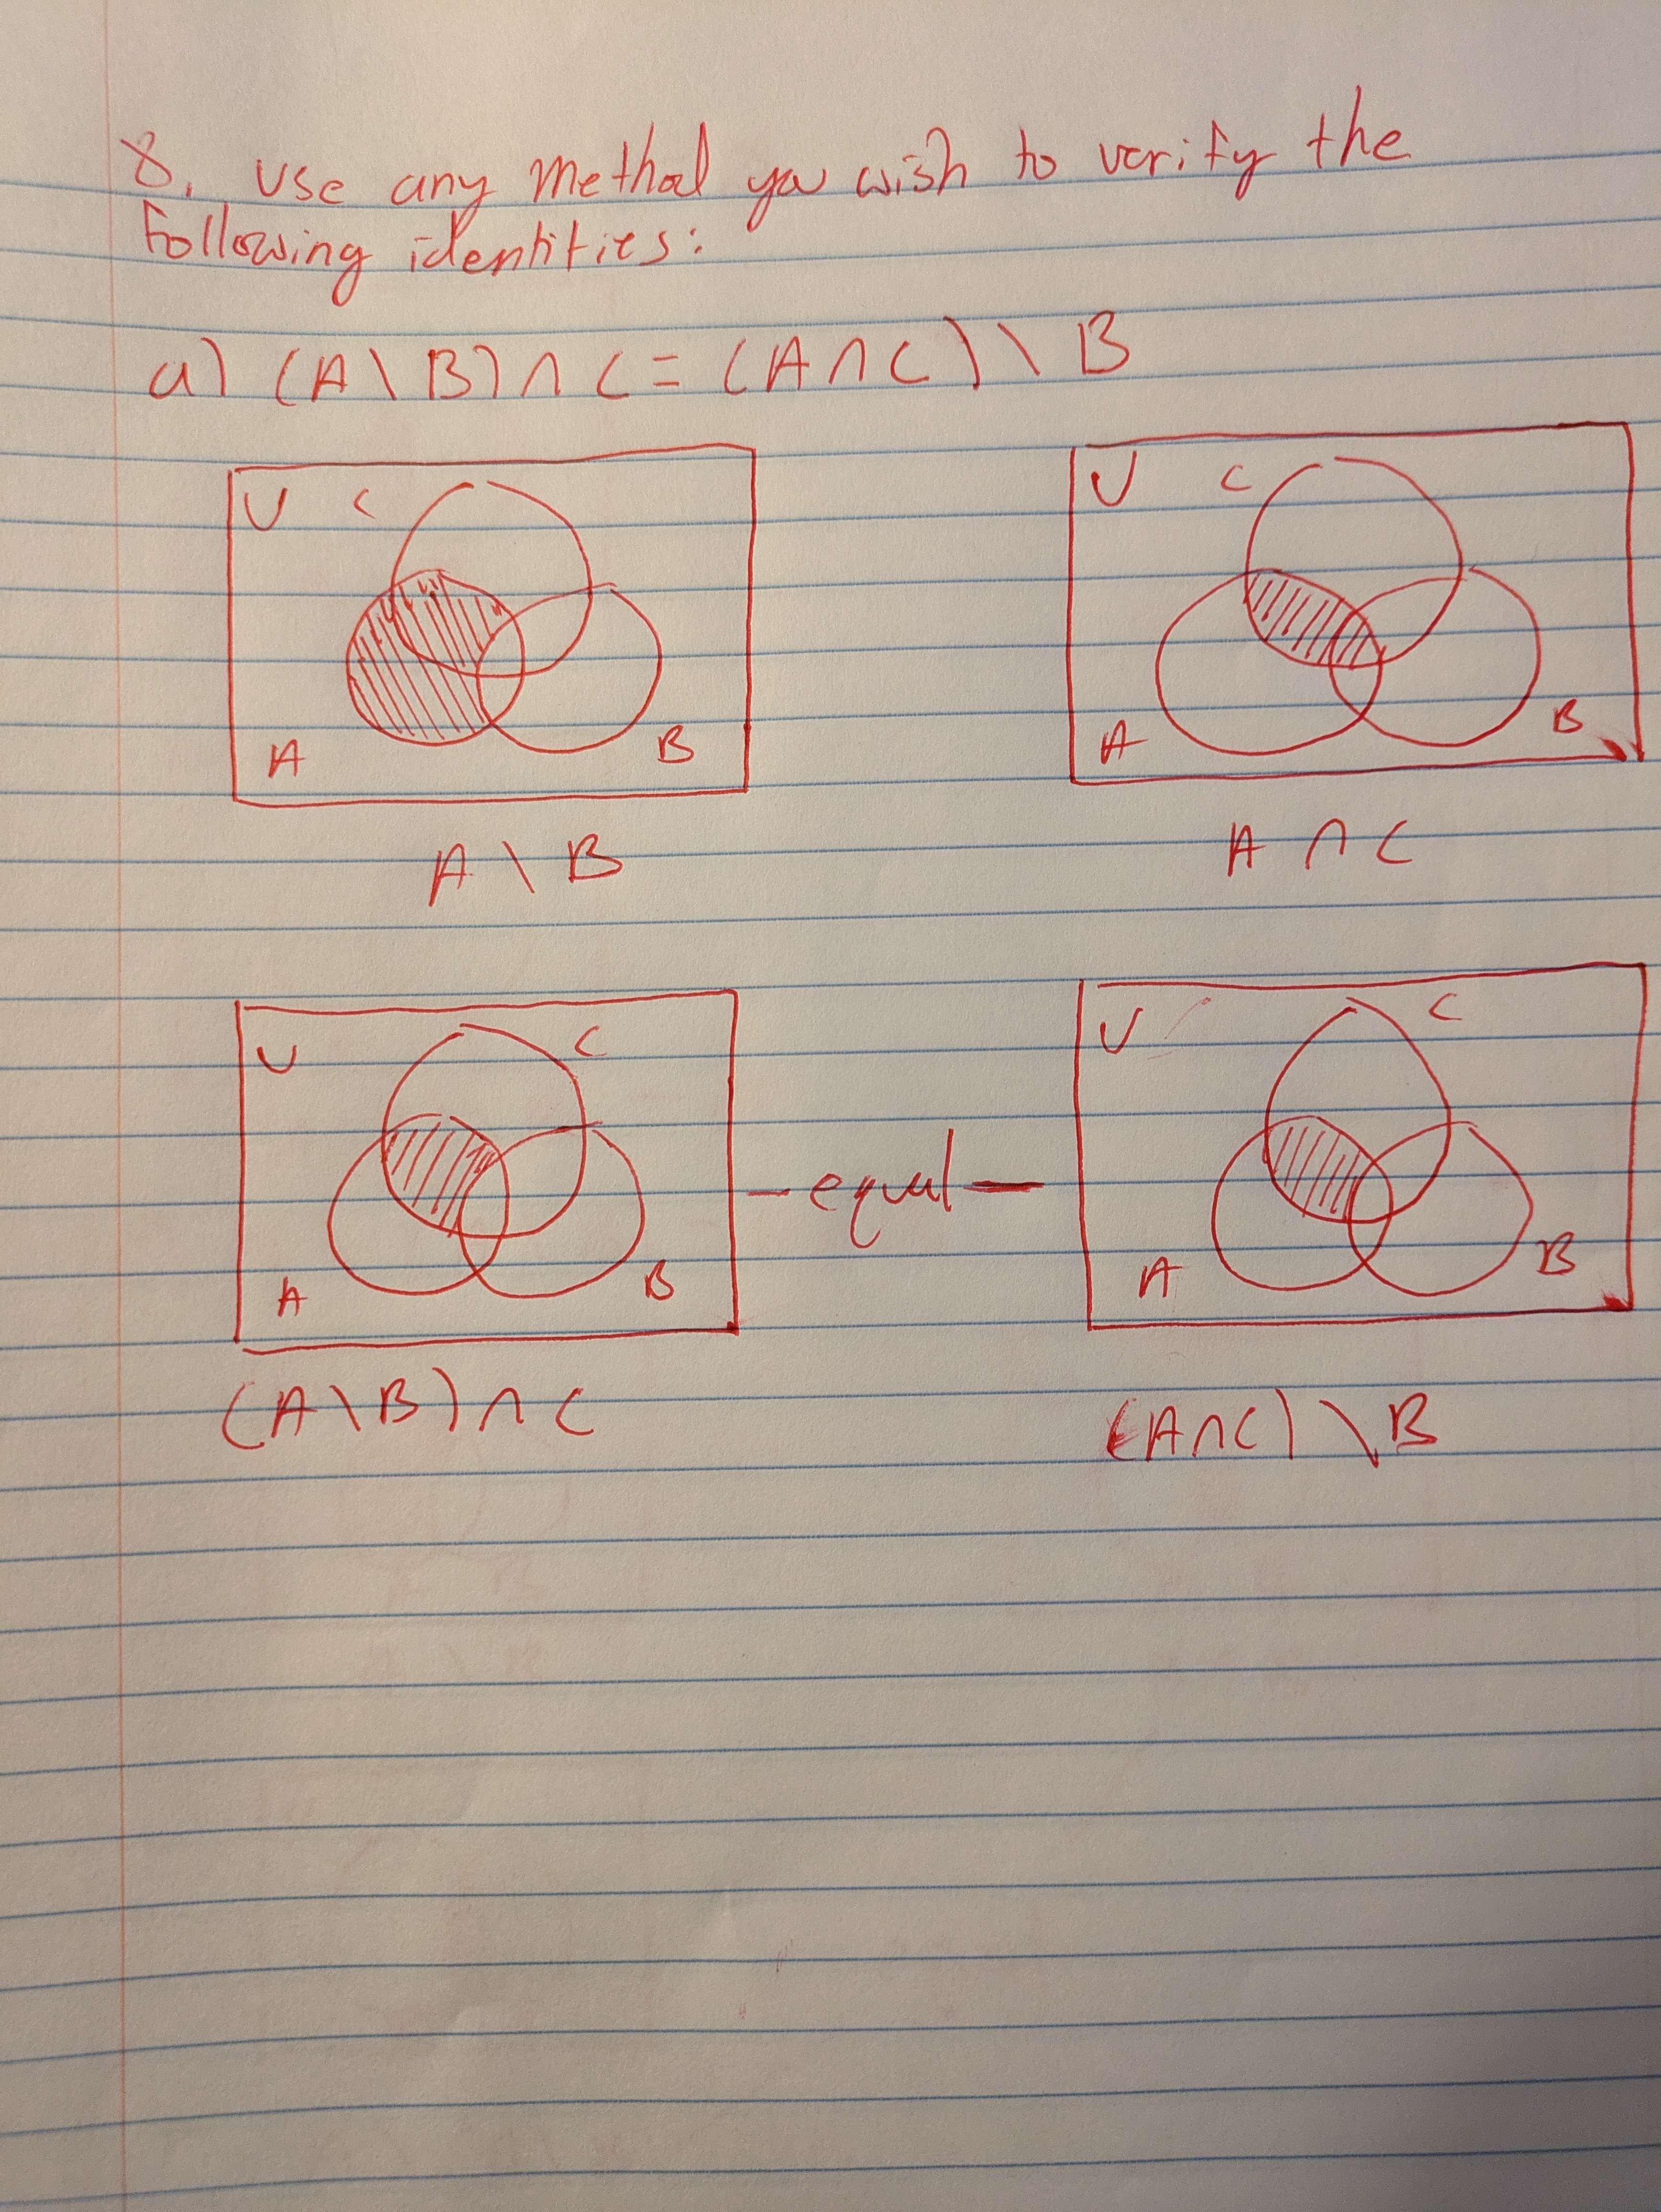
\includegraphics[width=0.8\textwidth]{images/1.2/7.jpg}
\end{figure}

\begin{tcolorbox}[title=Problem 9, breakable]
For each of the following sets, write out (using logical symbols) what it means
for an object $x$ to be an element of the set. Then determine which of these sets
must be equal to each other by determining which statements are equivalent. \\
(a) $(A \setminus B) \setminus C$ \\
(b) $A \setminus B \setminus C$ \\
(c) $(A \setminus B) \cup (A \cap C)$ \\
(d) $(A \setminus B) \cap (A \setminus C)$ \\
(e) $A \setminus (B \cup C)$ \\
\end{tcolorbox}

\textbf{Solution}
\begin{align*}
\text{Let } X &\equiv (x \in A) & \\
\text{Let } Y &\equiv (x \in B) & \\
\text{Let } Z &\equiv (x \in C) & \\& \\
\textbf{(a) } x \in (A \setminus B) \setminus C 
    &\equiv x \in (A \setminus B) \wedge x \not \in C & \\
    &\equiv (x \in A \wedge x \not \in B) \wedge x \not \in C & \\
    &\equiv (X \wedge \neg Y) \wedge \neg Z & \\
    &\equiv X \wedge \neg Y \wedge \neg Z & \\ 
\textbf{(b) } x \in A \setminus (B \setminus C) 
    &\equiv x \in A \wedge \neg(x \in B \setminus C) & \\
    &\equiv x \in A \wedge \neg(x \in B \wedge x \not \in C) & \\
    &\equiv X \wedge \neg(Y \wedge \neg Z) & \\
\textbf{(c) } x \in (A \setminus B) \cup (A \cap C) 
    &\equiv (x \in A \wedge x \not \in B) \vee (x \in A \wedge x \in C) & \\
    &\equiv (X \wedge \neg Y) \vee (X \wedge Z) & \\ 
\textbf{(d) } x \in (A \setminus B) \cap (A \setminus C) 
    &\equiv (x \in A \wedge x \not \in B) \wedge (x \in A \wedge x \not \in C) & \\
    &\equiv (X \wedge \neg Y) \wedge (X \wedge \neg Z) & \\ 
    &\equiv X \wedge \neg Y \wedge \neg Z & \\ 
\textbf{(e) } x \in A \setminus (B \cup C) 
    &\equiv x \in A \wedge \neg (x \in B \vee x \in C) & \\
    &\equiv X \wedge \neg (Y \vee Z) & \\
    &\equiv X \wedge (\neg Y \wedge \neg Z) 
\end{align*}

(a) and (d) are equal \\
(b), (c), and (e) are equal

\begin{tcolorbox}[title=Problem 10, breakable]
It was shown in this section that for any sets $A$ and $B$, $(A \cup B) \subseteq A$. \\
(a) Give an example of two sets $A$ and $B$ for which $(A \cup B) \setminus B \not = A$. \\
(b) Show that for all sets $A$ and $B$, $(A \cup B) \setminus B = A \setminus B$.
\end{tcolorbox}

\textbf{Problem 10 (a)}
\begin{align*}
A &= \{1, 2, 3\} & \\
B &= \{4, 2, 5\} & \\
A \cup B &= \{1, 2, 3, 4, 5\} & \\
(A \cup B) \setminus B &= \{1, 3\} & \\
\{1, 3\} &\not = A & \\
\end{align*}

Want to show $x \in (A \cup B) \setminus B$ is equivalent to $x \in A \setminus B$ \\ \\
\textbf{Problem 10 (b)}
\begin{align*}
x \in (A \cup B) \setminus B 
&\equiv x \in (A \cup B) \wedge x \notin B &&\text{(def. of set difference)} \\
&\equiv (x \in A \vee x \in B) \wedge x \notin B &&\text{(def. of union)} \\
&\equiv (x \notin B \wedge x \in B) \vee (x \notin B \wedge x \in A) &&\text{(distributive)} \\
&\equiv (x \notin B \wedge x \in A) &&\text{(contradiction)} \\
&\equiv (x \in A \wedge x \notin B) &&\text{(commutative)} \\
&\equiv x \in A \setminus B &&\text{(def. of set difference)} \\
\end{align*}

\begin{tcolorbox}[title=Problem 11, breakable]
Suppose $A$ and $B$ are sets. \\
Is it necessarily true that $(A \setminus B) \cup B = A$? \\
If not, is one of these sets necessarily a subset of the other? \\
Is $(A \setminus B) \cup B$ always equal to either $A \setminus B$ or $A \cup B$.
\end{tcolorbox}

\textbf{Problem 11}

No it is not necessarily true.
\begin{align*}
A &= \{1, 2\} \\
B &= \{3\} \\
(A \setminus B) &= \{1, 2\} \\
(A \setminus B) \cup B &= \{1, 2, 3\} \\
A &\not = \{1, 2, 3\}
\end{align*}

It is not always equal to $A \setminus B$ as shown above.

It is always equal to $A \cup B$. Proof:
\begin{align*}
x \in (A \setminus B) \cup B &\equiv x \in (A \setminus B) \vee x \in B &&\quad \text{def. of union} \\
&\equiv (x \in A \wedge x \not \in B) \vee x \in B &&\quad \text{def. of set difference} \\
&\equiv (x \in B \vee x \not \in B) \wedge (x \in B \vee x \in A) &&\quad \text{distributive} \\
&\equiv x \in B \vee x \in A &&\quad \text{tautology} \\
&\equiv x \in A  \vee x \in B &&\quad \text{commutative} \\
&\equiv x \in (A \cup B) &&\quad \text{def. of union} \\
\end{align*}

$A$ is always a subset of $(A \setminus B) \cup B$. 

From above $(A \setminus B) \cup B \equiv A \cup B$.

From def. of union that means $x \in A$.

$(A \setminus B) \cup B $ is not always a subset of $A$.

From above $(A \setminus B) \cup B \equiv A \cup B$.

Therefore, $x$ could be in $B$ and not in $A$ and still exist in $(A \setminus B) \cup B$.

\textbf{Problem 12:}
\begin{figure}[H]
    \centering
    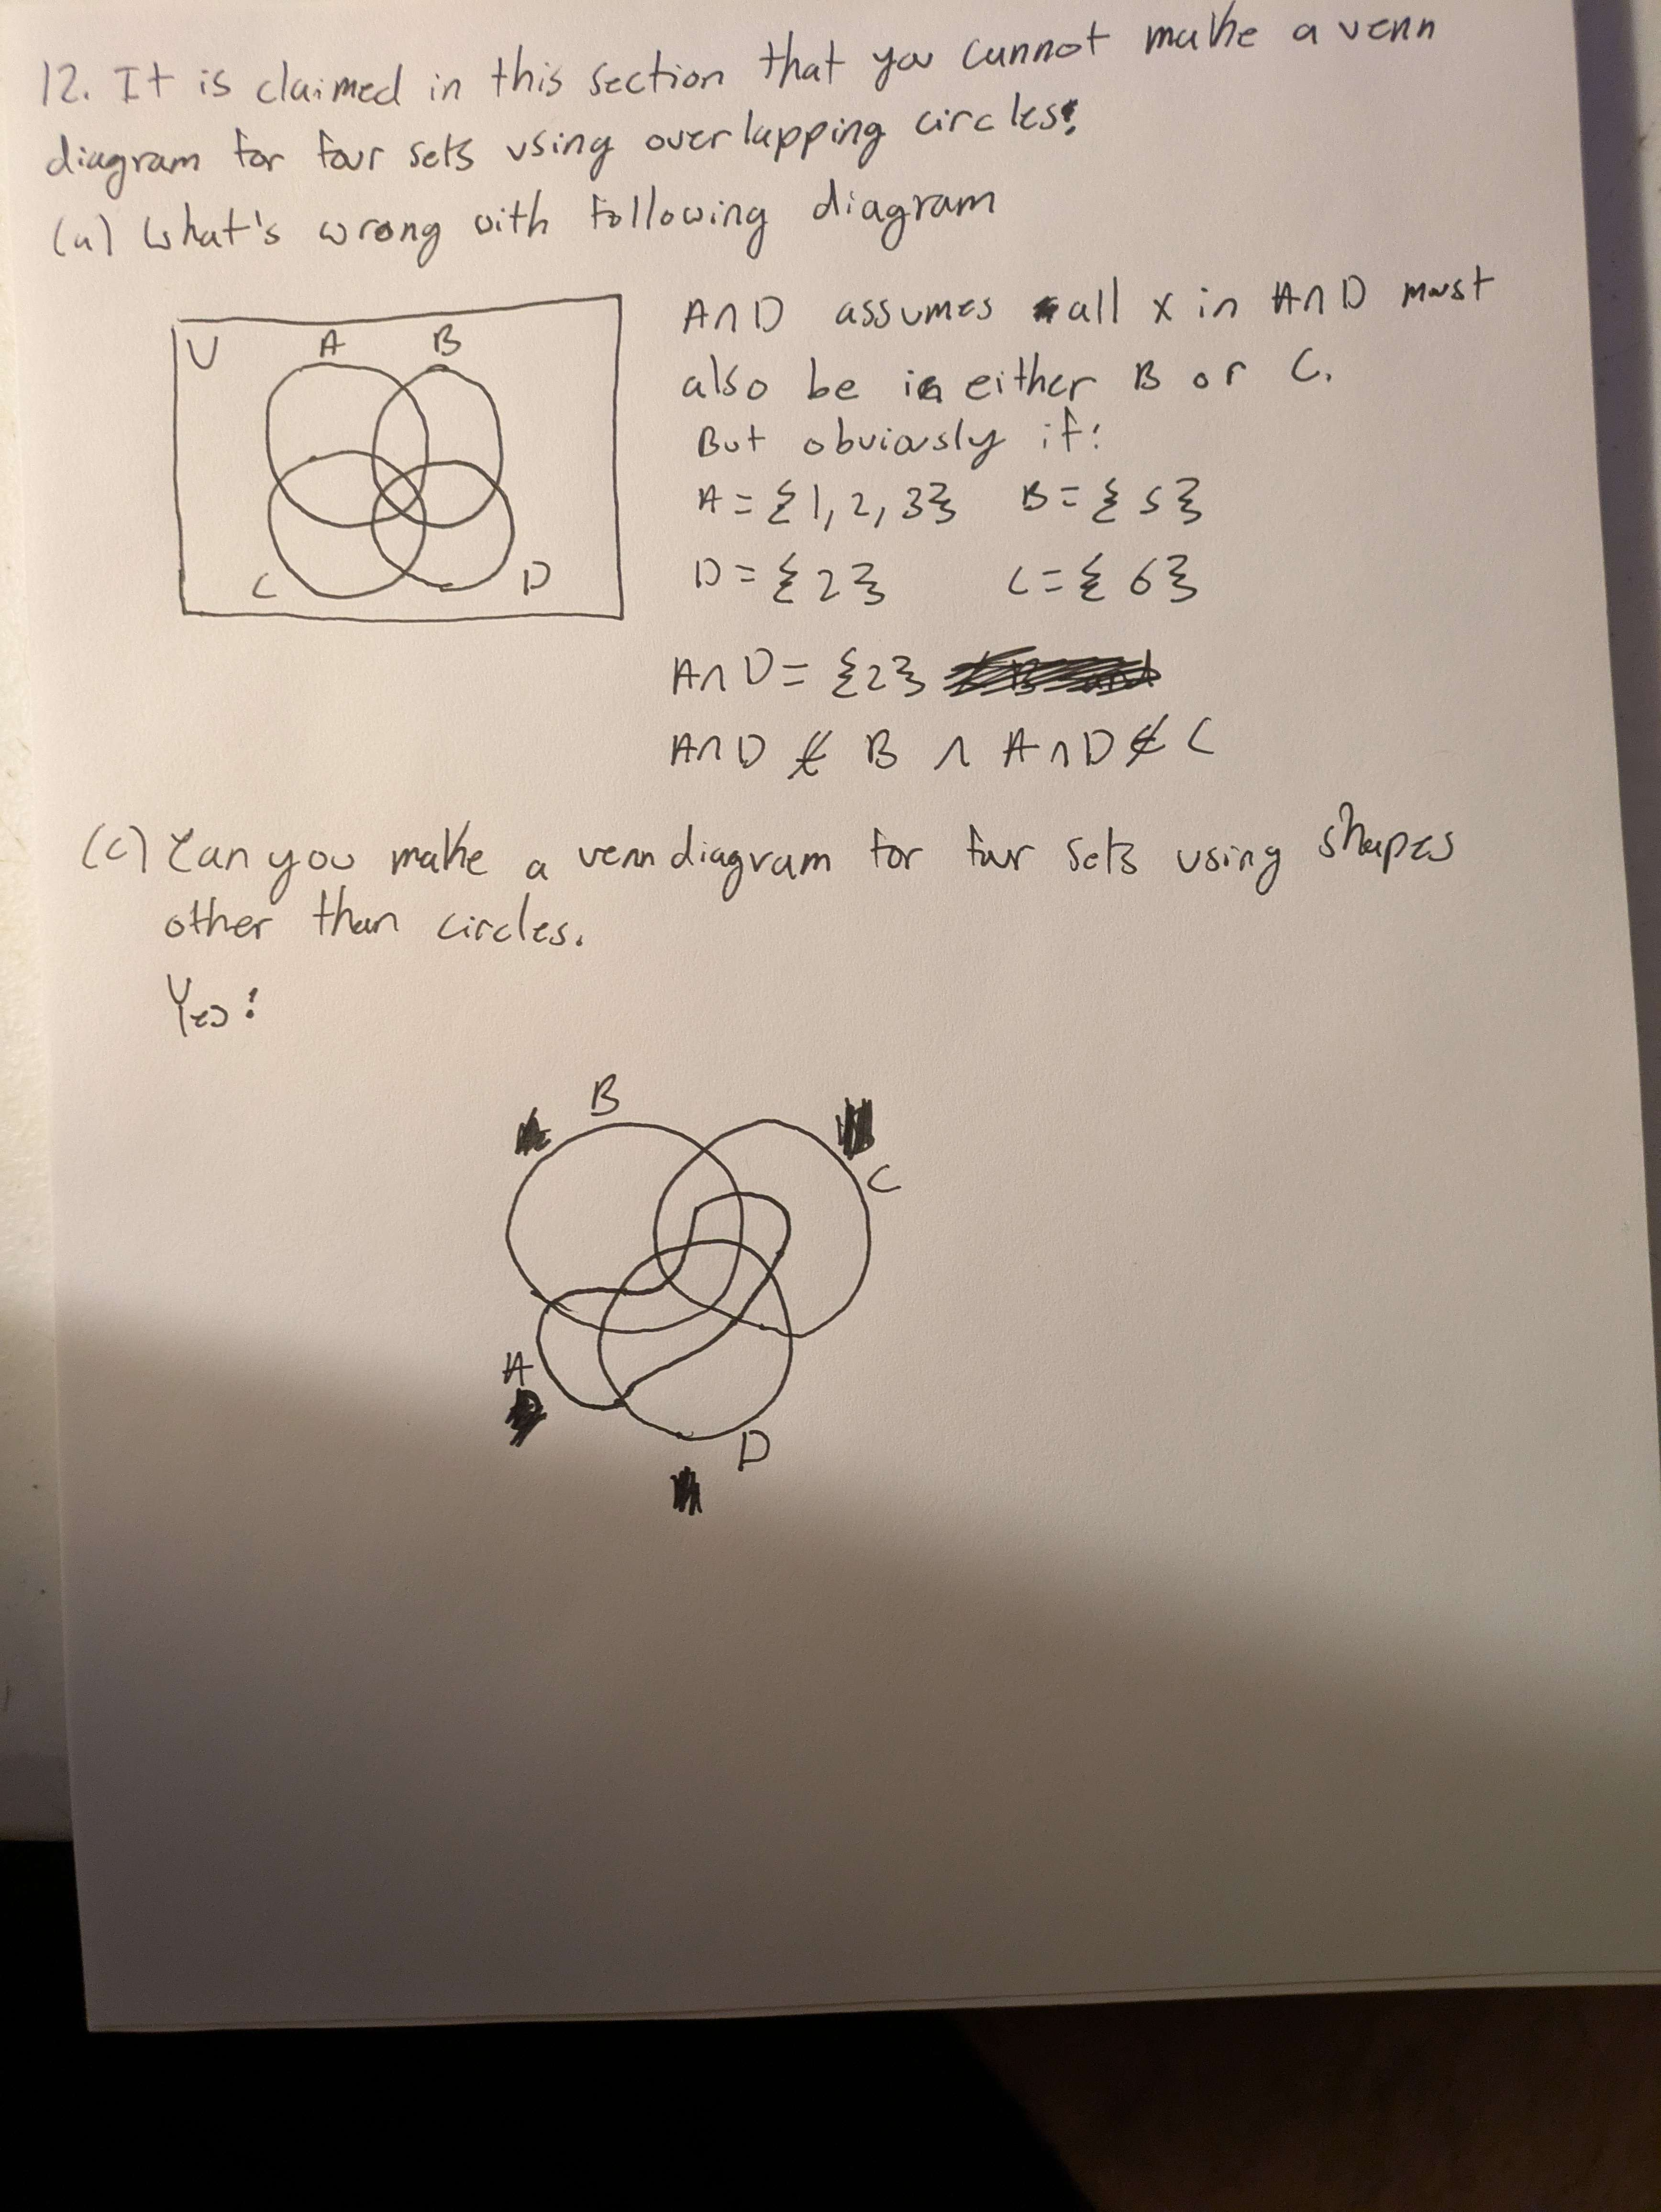
\includegraphics[width=0.8\textwidth]{images/1.2/8.jpg}
\end{figure}

\textbf{Problem 13:}
\begin{figure}[H]
    \centering
    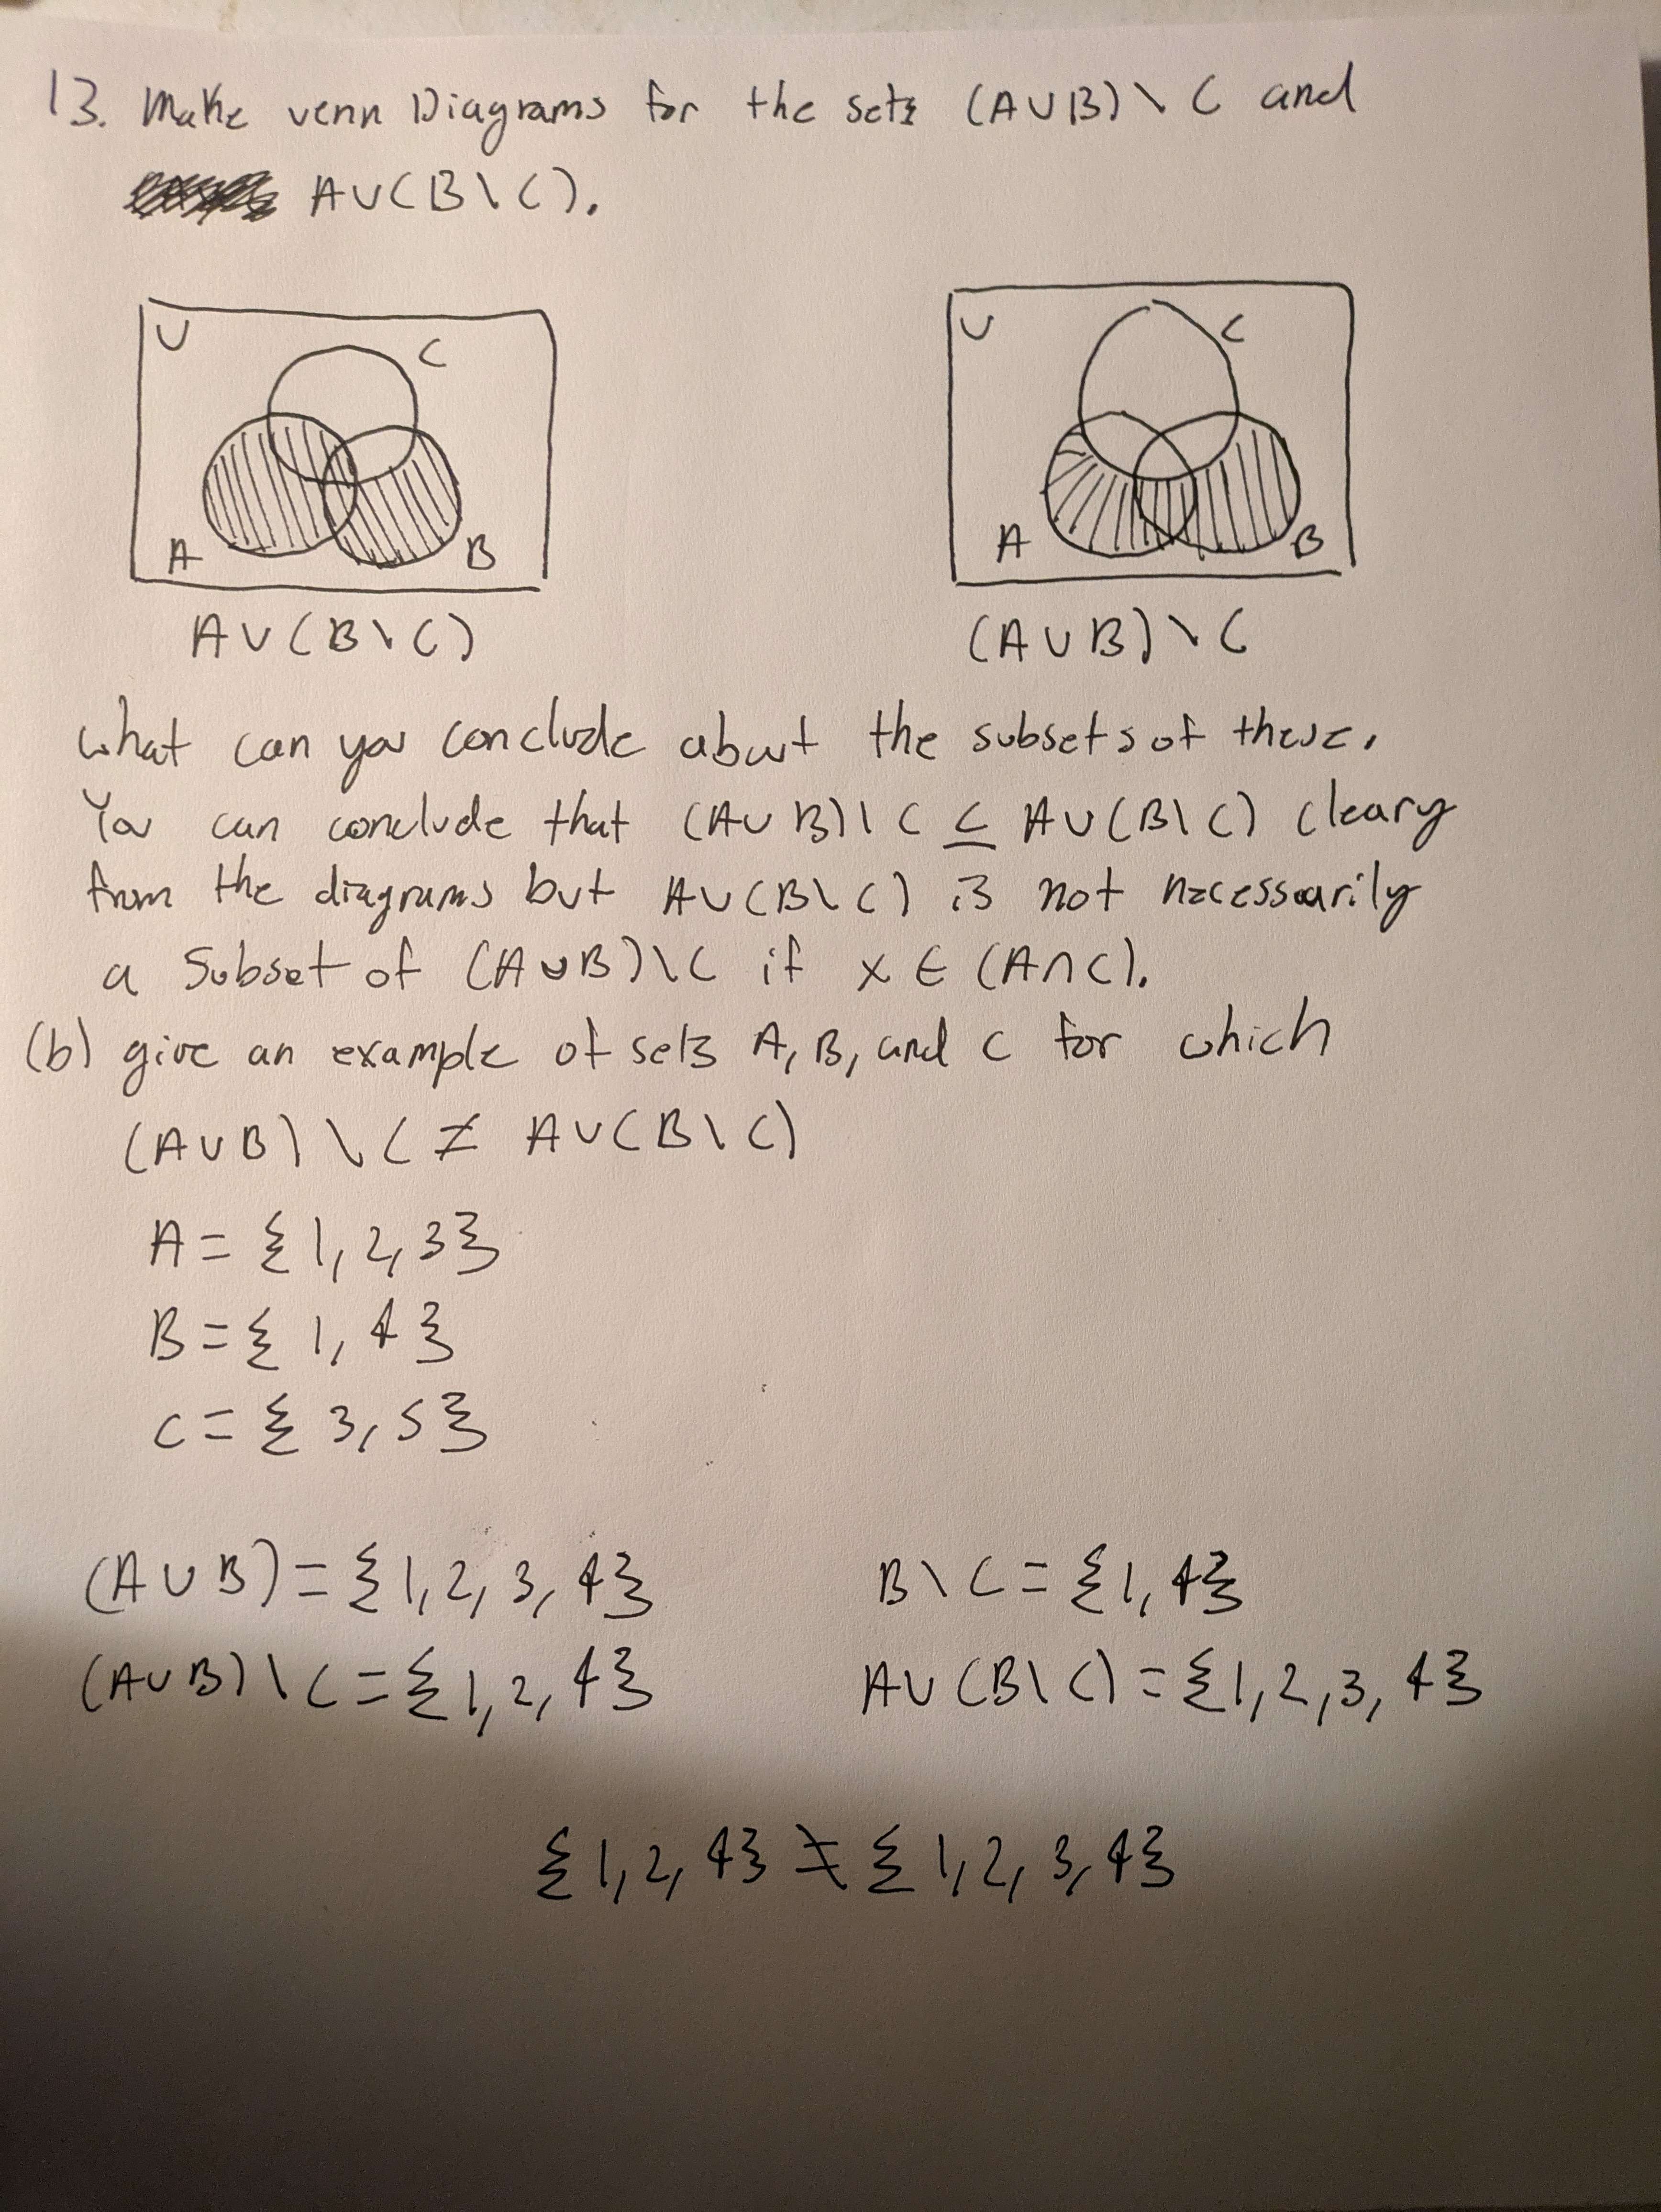
\includegraphics[width=0.8\textwidth]{images/1.2/9.jpg}
\end{figure}

\textbf{Problem 14:}
\begin{figure}[H]
    \centering
    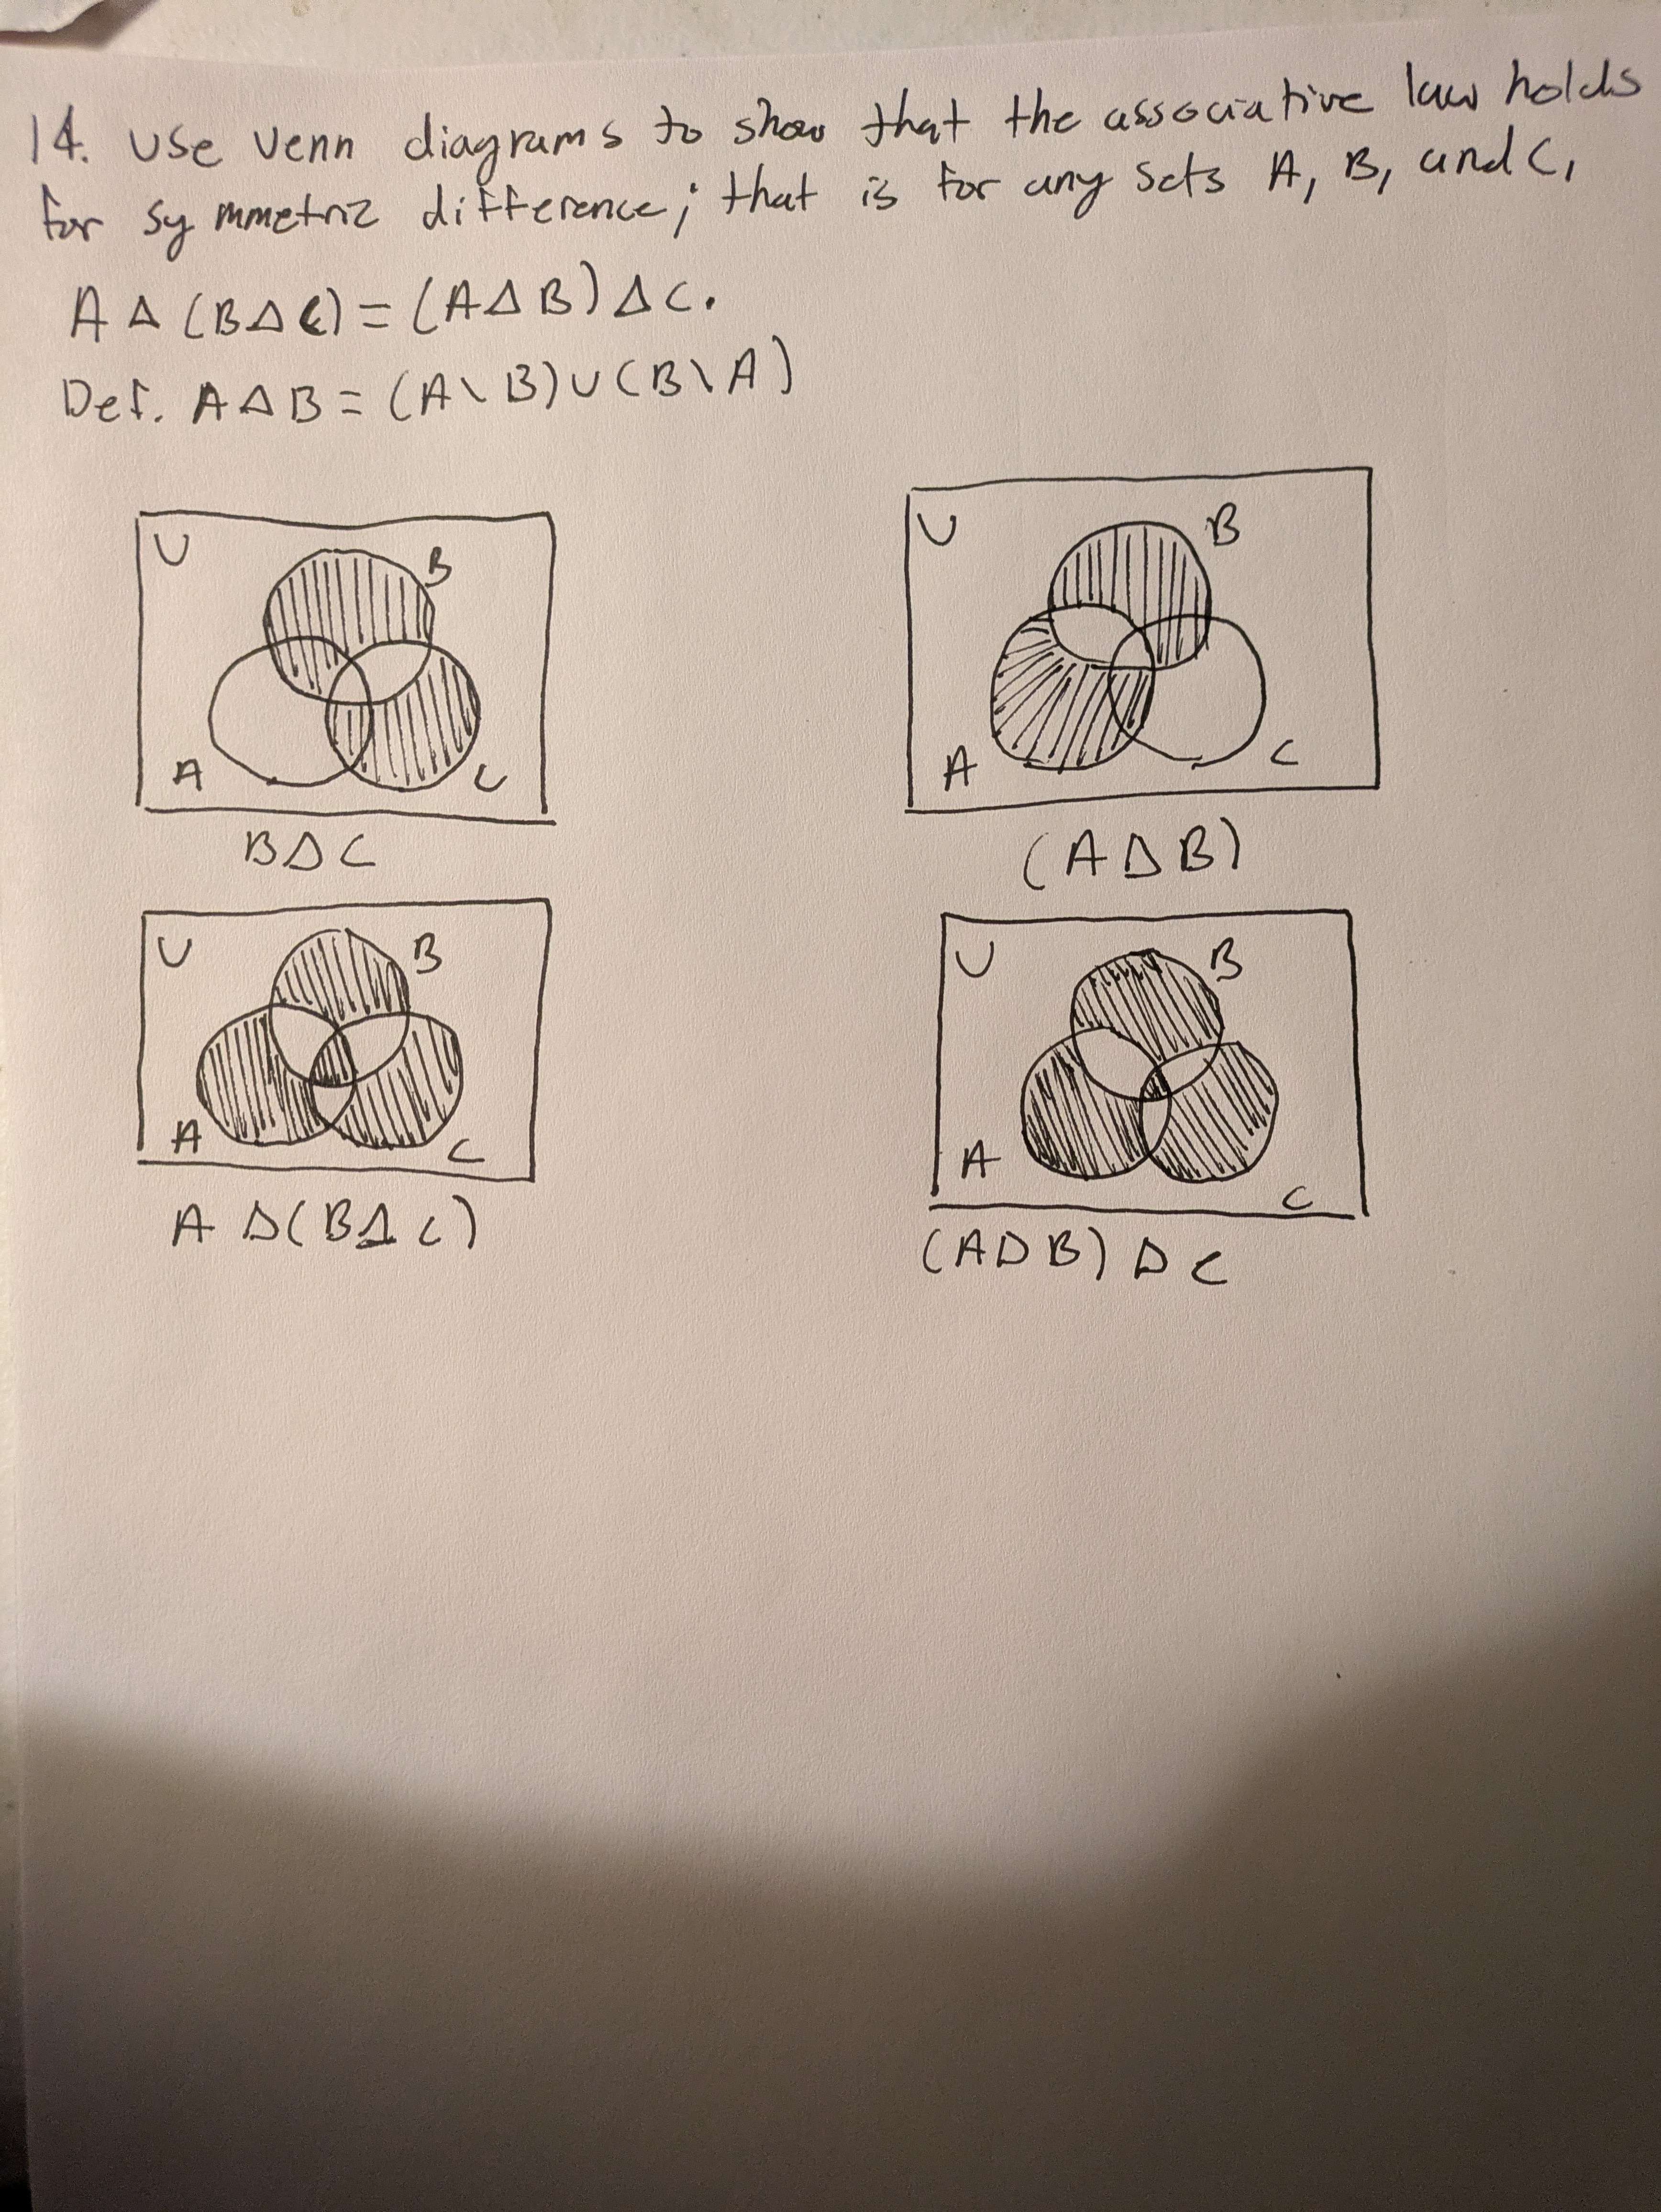
\includegraphics[width=0.8\textwidth]{images/1.2/10.jpg}
\end{figure}
\begin{figure}[H]
    \centering
    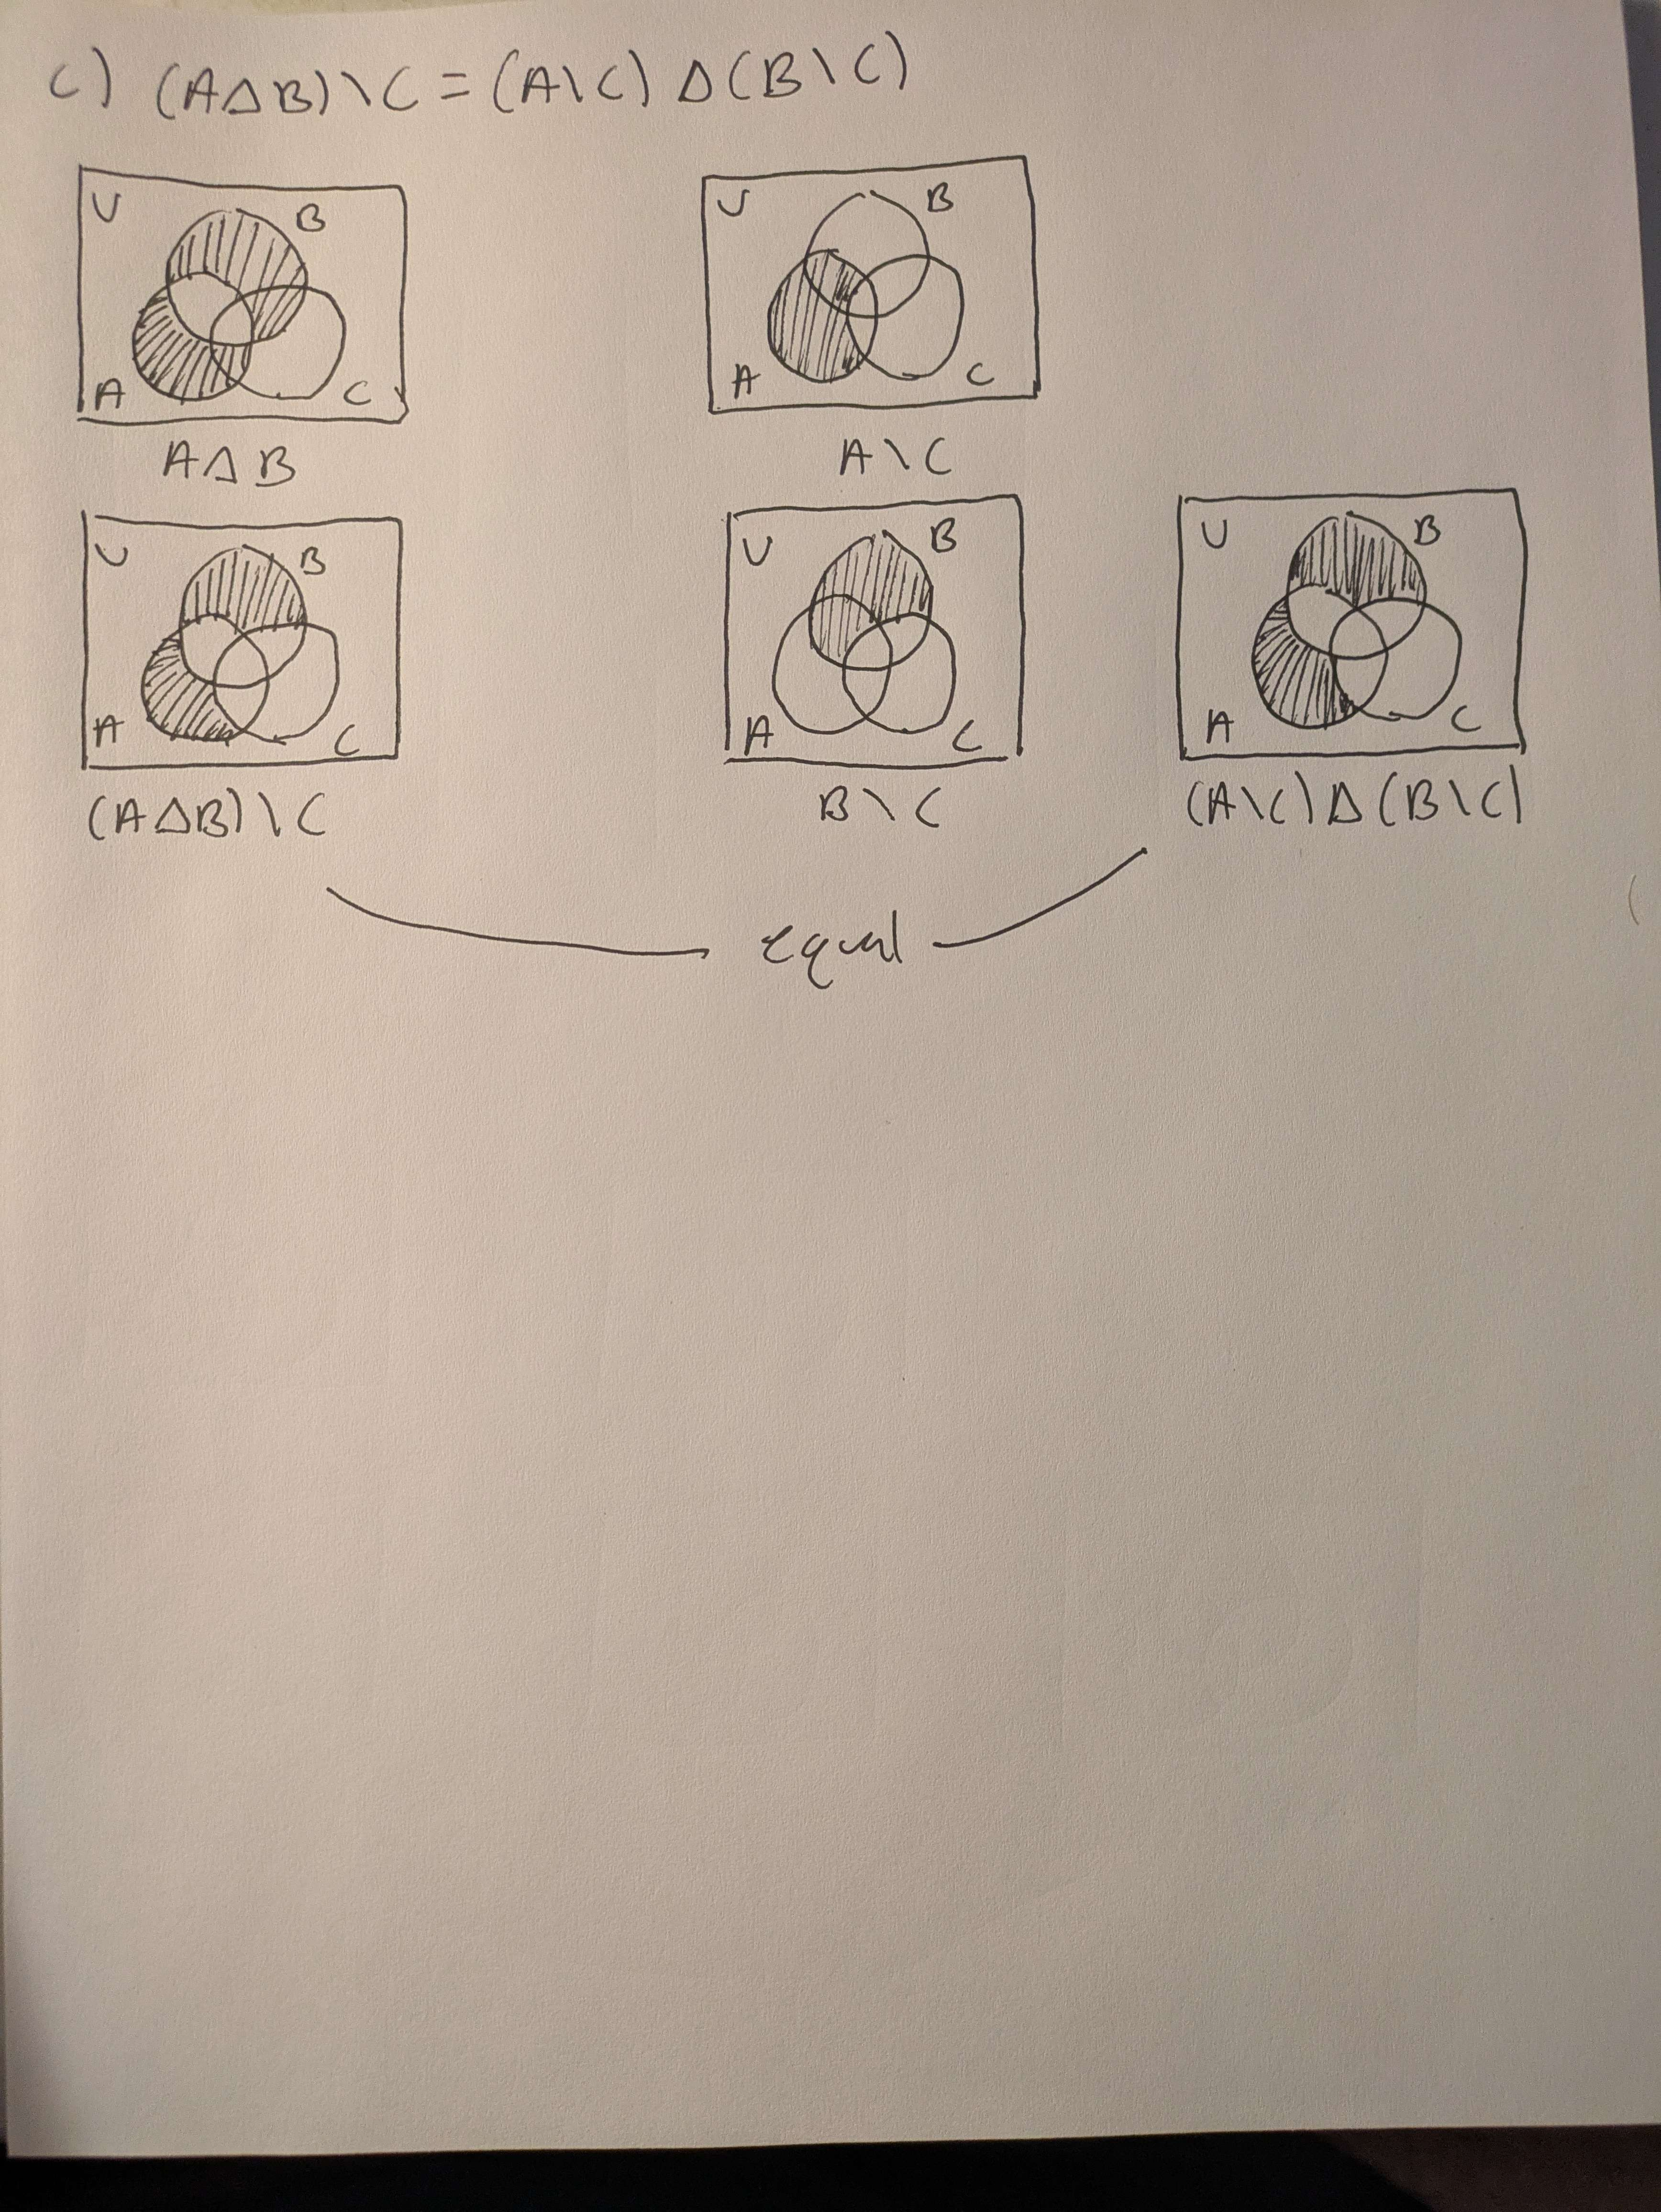
\includegraphics[width=0.8\textwidth]{images/1.2/11.jpg}
\end{figure}
\begin{figure}[H]
    \centering
    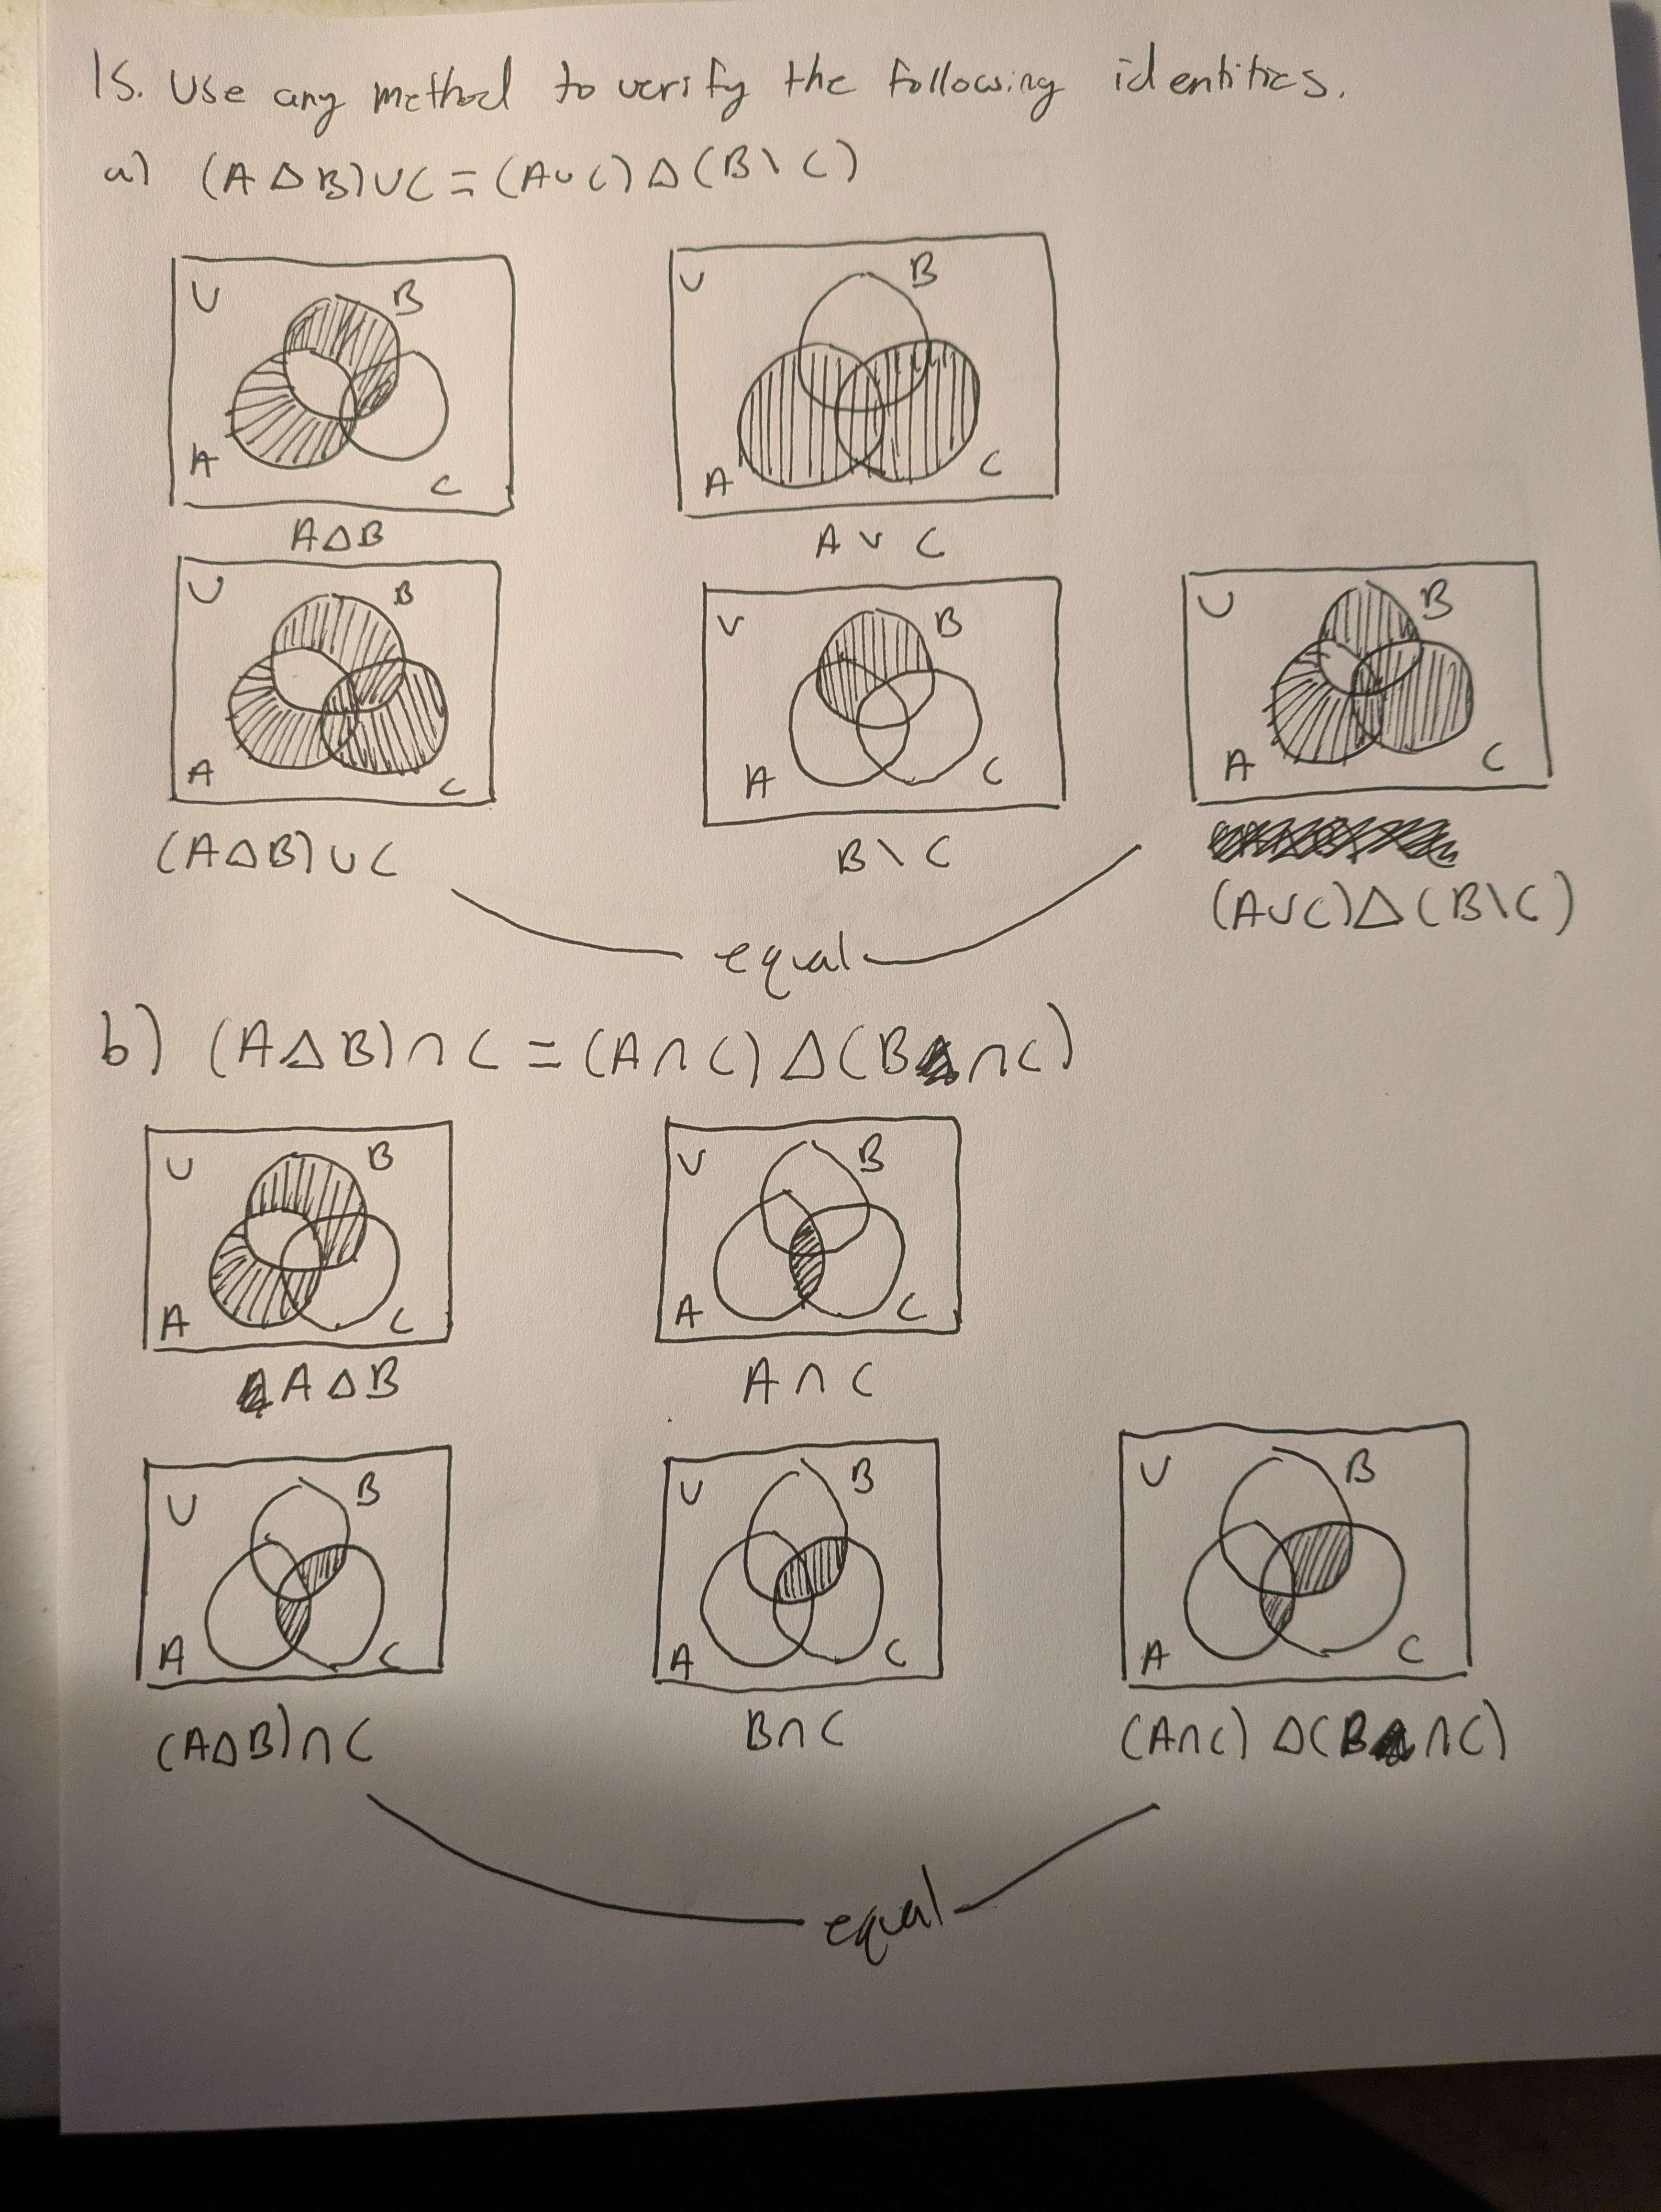
\includegraphics[width=0.8\textwidth]{images/1.2/12.jpg}
\end{figure}

\begin{tcolorbox}[title=Problem 16 (a), breakable]
Use any method you wish to verify the following identity.
$(A \cup B) \triangle C = (A \triangle C) \triangle (B \setminus A)$
\end{tcolorbox}

\begin{proof}
First note that commutativity holds for symmetric difference
\begin{align*}
A \triangle B &\equiv (A \cup B) \setminus (A \cap B) && \quad \text{def. of symmetric difference} \\
&\equiv (B \cup A) \setminus (B \cap A)  && \quad \text{commutative} \\
&\equiv B \triangle A && \quad \text{def. of symmetric difference}
\end{align*}
Also note $x \in A \cup B \equiv x \in A \triangle (B \setminus A)$.
Let $X \equiv x \in A$, $Y \equiv x \in B$.
Starting with the rhs
\begin{align*}
x \in A \triangle (B \setminus A) &\equiv x \in (A \cup (B \setminus A)) \setminus (A \cap (B \setminus A)) && \quad \text{def. of symmetric difference} \\
&\equiv [X \vee (Y \wedge \neg X)] \wedge \neg [X \wedge (Y \wedge \neg X)] && \quad \text{def. of union, intersection, set difference} \\
&\equiv [(X \vee \neg X) \wedge (X \vee Y)] \wedge \neg [(X \wedge \neg X) \wedge (X \wedge Y)] && \quad \text{distributive} \\
&\equiv [X \vee Y] \wedge \neg [(X \wedge \neg X) \wedge (X \wedge Y)] && \quad \text{tautology} \\
&\equiv [X \vee Y] && \quad \text{contradiction} \\
&\equiv X \vee Y && \quad \text{} \\
&\equiv x \in X \cup Y && \quad \text{def. of union}
\end{align*}
Now
\begin{align*}
(A \cup B) \triangle C &\equiv (A \triangle (B \setminus A)) \triangle C && \\
&\equiv A \triangle ((B \setminus A) \triangle C) && \quad \text{associative} \\
&\equiv A \triangle (C \triangle (B \setminus A)) && \quad \text{commutativity} \\
&\equiv (A \triangle C) \triangle (B \setminus A) && \quad \text{associative}
\end{align*}
Therefore, the identity $(A \cup B) \triangle C = (A \triangle C) \triangle (B \setminus A)$ holds.
\end{proof}
\begin{figure}[H]
    \centering
    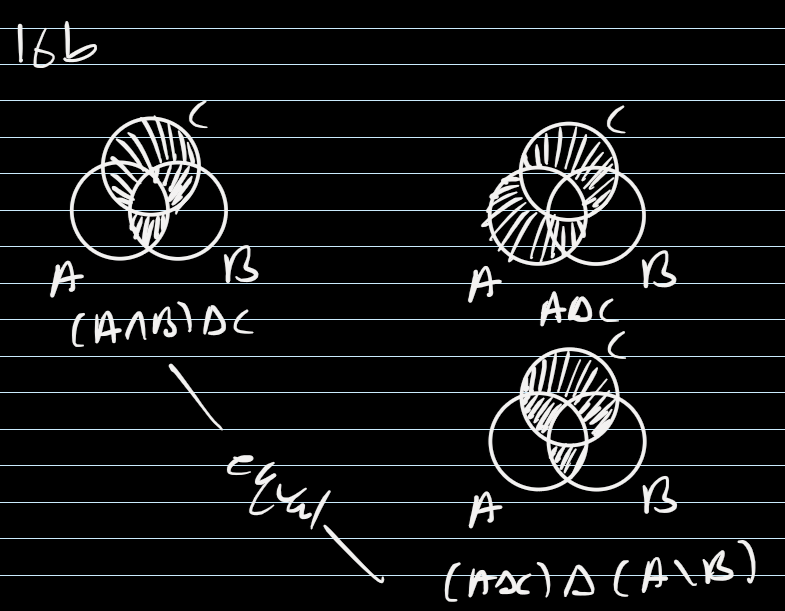
\includegraphics[width=0.8\textwidth]{images/1.2/26.PNG}
\end{figure}
\begin{figure}[H]
    \centering
    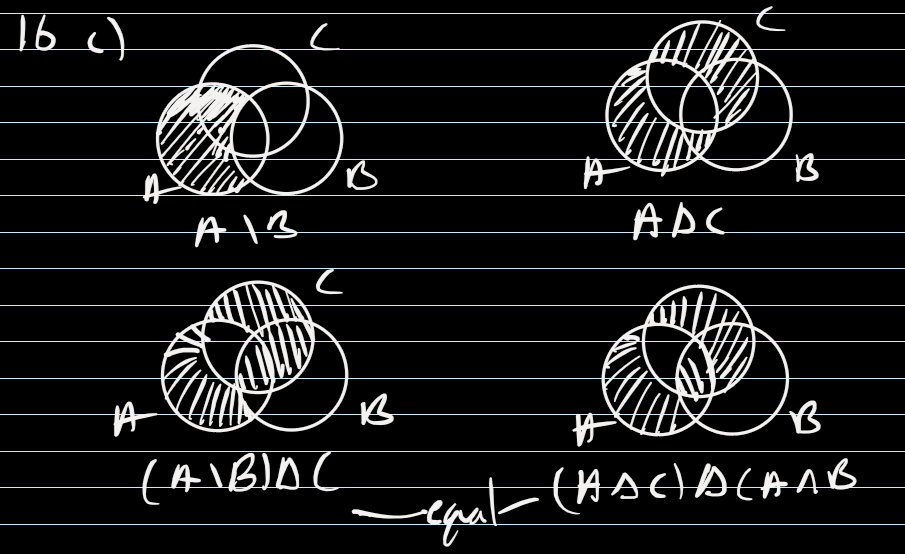
\includegraphics[width=0.8\textwidth]{images/1.2/27.PNG}
\end{figure}

\textbf{Problem 17:}
\begin{figure}[H]
    \centering
    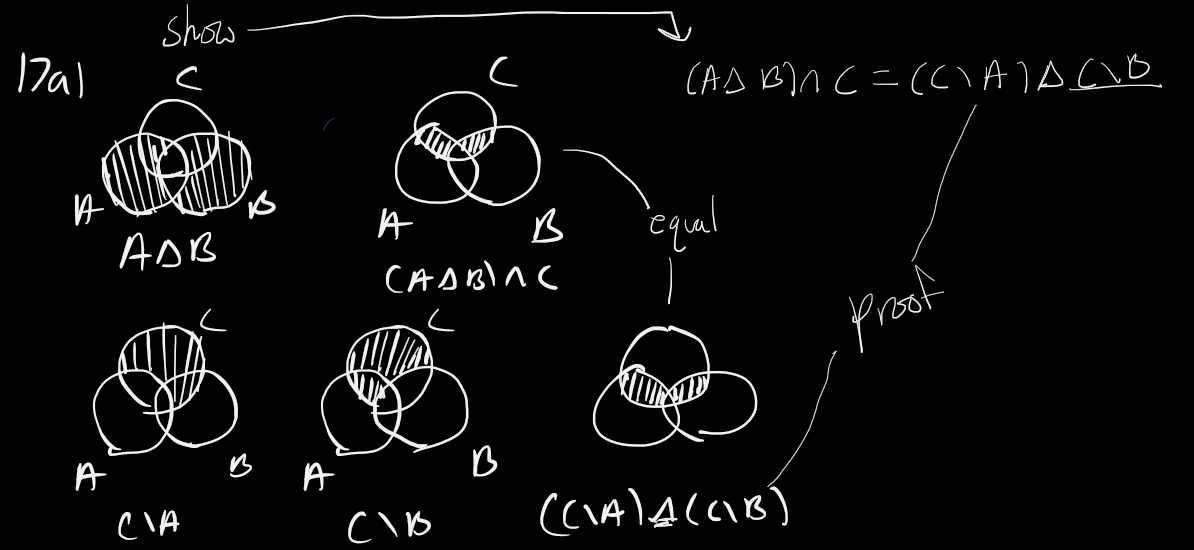
\includegraphics[width=0.8\textwidth]{images/1.2/28.PNG}
\end{figure}
\begin{figure}[H]
    \centering
    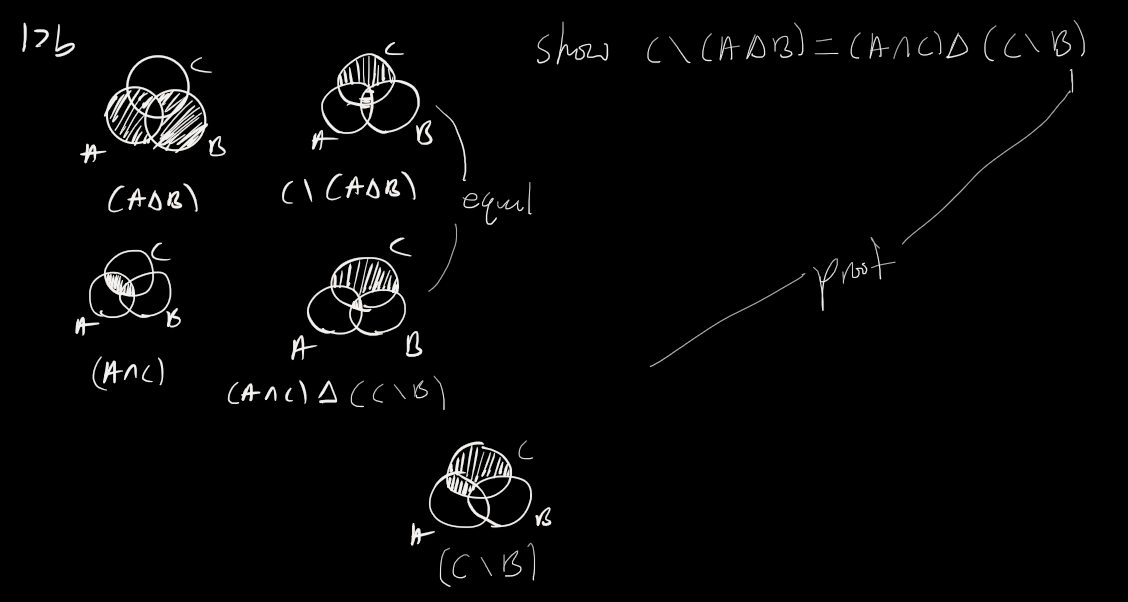
\includegraphics[width=0.8\textwidth]{images/1.2/29.PNG}
\end{figure}
\begin{figure}[H]
    \centering
    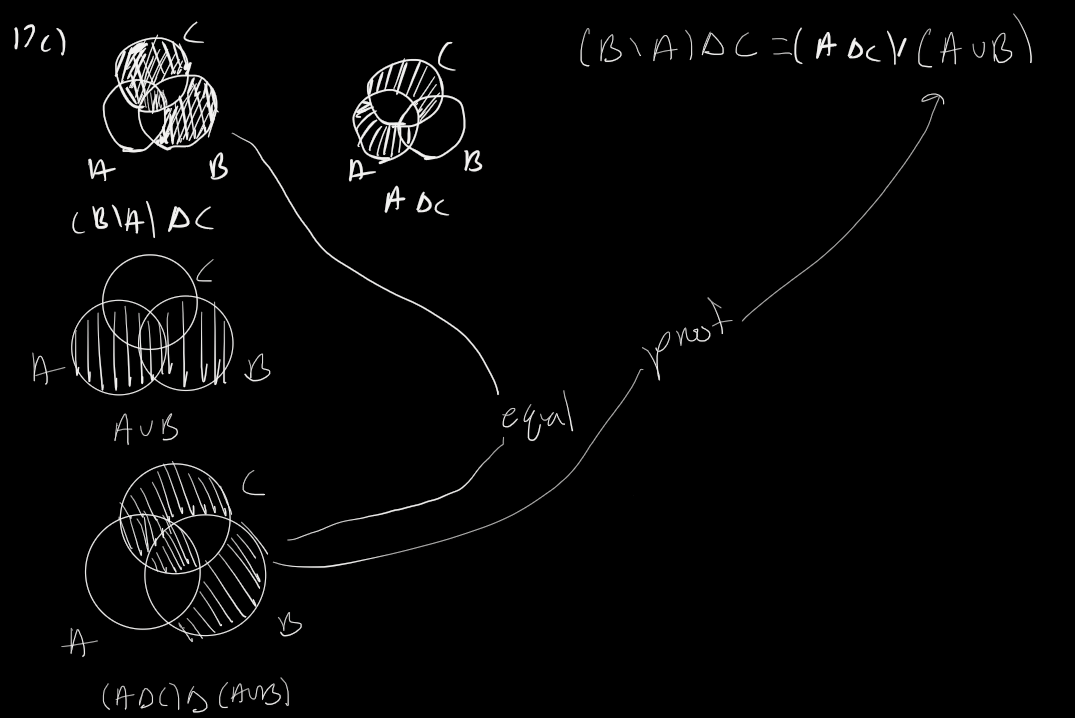
\includegraphics[width=0.8\textwidth]{images/1.2/30.PNG}
\end{figure}

\subsection{The Conditional and Biconditional Connectives}

\begin{tcolorbox}[title=Problem 2, breakable]
Analyze the logicla forms of the following statements: \\
(a) Mary will sell her house only if she can get a good price and find a nice apartment. \\
(b) Having both a good credit history and an adequate down payment is a necessary
condition for getting a mortgage. \\
(c) John will drop out of school, unless someone stops him .(Hint: First try to
rephrase this using the words \textit{if} and \textit{then} instead of \textit{unless}). \\
(d) If $x$ is divisible by either $4$ or $6$, then it isn't prime.
\end{tcolorbox}

\textbf{Problem (a)} \\
Let \textit{G} stand for the statement, "Mary can get a good price". \\
Let \textit{F} stand for the statement, "Mary can find a nice aparment". \\
Let \textit{S} stand for the statement, "Mary will sell her house". \\ \\
$S \rightarrow G \wedge F$ \\ \\
\textbf{Problem (b)} \\
Let \textit{C} stand for the statement, "Having a good credit score history". \\
Let \textit{A} stand for the statement, "Having an adequate downpayment on the house." \\
Let \textit{M} stand for the statement, "Getting a mortgage". \\ \\
$M \rightarrow C \wedge A$ \\ \\
\textbf{Problem (c)} \\
Let \textit{D} stand for the statement, "John drops out of school". \\
Let \textit{S} stand for the statement, "Someone stops him". \\ \\
$S \rightarrow \neg D$ \\ \\
\textbf{Problem (d)} \\
Let \textit{X} stand for the statement, "x is divisible by 4". \\
Let \textit{Y} stand for the statement, "x is divisible by 6". \\
Let \textit{Z} stand for the statement, "x is a prime". \\ \\
$X \vee Y \rightarrow \neg Z$.

\begin{tcolorbox}[title=Problem 3, breakable]
Analyze the logical form of the following statement: \\
(a) If it is raining, then it is windy and the sun is not shining. \\
Now analyze the following statements. Also, for each statement determine
whether the statement is equivalent to either statement (a) or its converse. \\
(b) It is windy and not sunny only if it is raining. \\
(c) Rain is a sufficient condition for wind with no sunshine. \\
(d) Rain is a necessary condition for wind with no sunshine. \\
(e) It's not raining, if either the sun is shining or it's not windy. \\
(f) Wind is a necessary condition for it to be rainy, and so is a lack of sunshine. \\
(g) Either it is windy only if it is rainy, or it is not sunny only if it is raining.
\end{tcolorbox}

\textbf{Solution (a)} \\
Let \textit{R} stand for the statement, "It is raining". \\
Let \textit{W} stand for the statement, "It is windy". \\
Let \textit{S} stand for the statement, "The sun is shining". \\ \\
$R \rightarrow (W \wedge \neg S)$ \\ \\
\textbf{Solution (b)} \\ \\
$(W \wedge \neg S) \rightarrow R$ Equivalent to (a) converse. \\ \\
\textbf{Solution (c)} \\ \\
$R \rightarrow (W \wedge \neg S)$ Equivalent to (a). \\ \\
\textbf{Solution (d)} \\ \\
$(W \wedge \neg S) \rightarrow R$ Equivalent to (a) converse. \\ \\
\textbf{Solution (e)} \\ \\
$(S \vee \neg W) \rightarrow \neg R$ \\
$R \rightarrow (W \wedge \neg S)$ Equivalent to (a) \\ \\
\textbf{Solution (f)} \\ \\
$R \rightarrow (W \wedge \neg S)$ Equivalent to (a) \\ \\
\textbf{Solution (g)} \\ \\
$(W \wedge \neg S) \rightarrow R$ Equivalent to (a) converse

\begin{tcolorbox}[title=Problem 5, breakable]
Use truth tables to determine whether or not the following arguments are valid: \\
(a) If Jones is convicted then he will go to prison. Jones will be convicted only if 
Smith testifies against him. Therefore, Jones won't go to prison unless Smith testifies
against him. \\
(b) Either the Democrats or the Republicans will have a majority in the Senate,
but not both. Having a Democratic majority is a necessary condition for the bill to
pass. Therefore, if the Republicans have a majority in the Senate then the bill
won't pass.
\end{tcolorbox}

\begin{figure}[H]
    \centering
    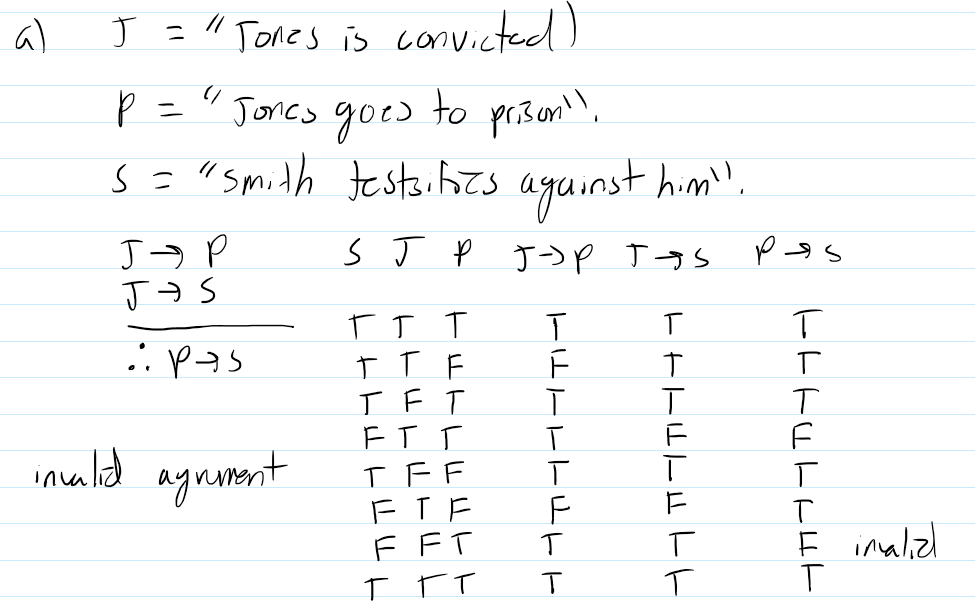
\includegraphics[width=0.8\textwidth]{images/1.2/31.PNG}
\end{figure}
\begin{figure}[H]
    \centering
    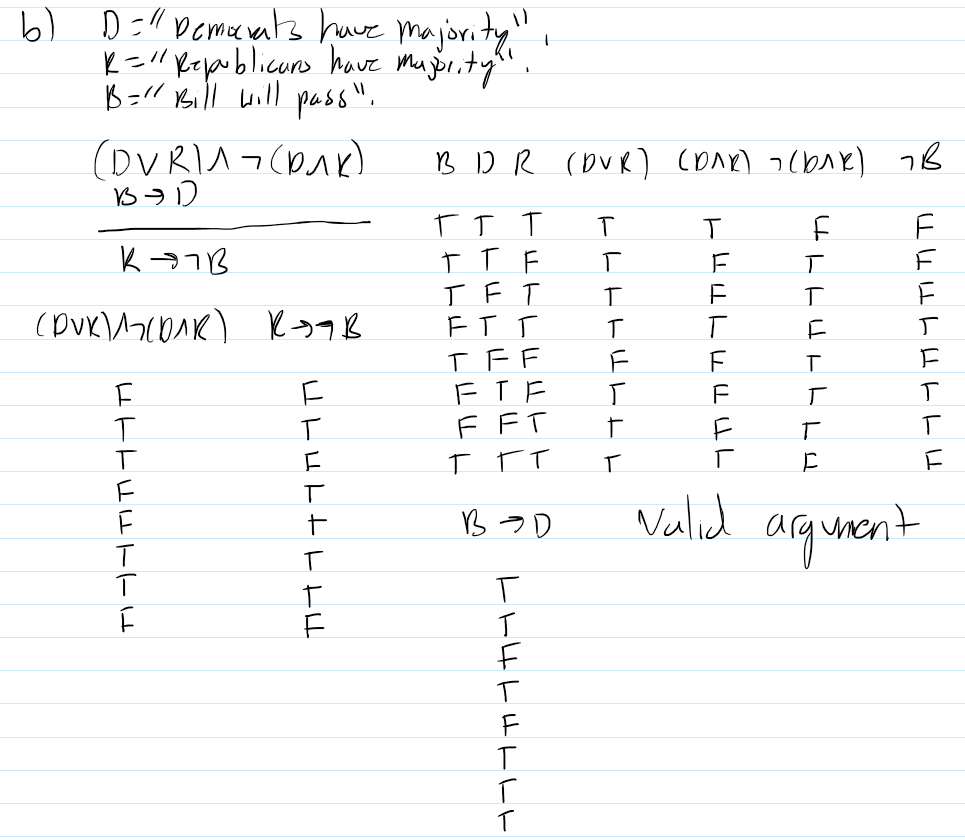
\includegraphics[width=0.8\textwidth]{images/1.2/32.PNG}
\end{figure}

\begin{tcolorbox}[title=Problem 6 (a), breakable]
Show that $P \leftrightarrow Q$ is equivalent to
$(P \wedge A) \vee (\neg P \wedge \neg Q)$.
\end{tcolorbox}

\begin{proof}
\begin{align*}
P \leftrightarrow Q &\equiv 
    (P \rightarrow Q) \wedge (Q \rightarrow P) && \quad \text{def. of iff} \\
&\equiv (\neg P \vee Q) \wedge (\neg Q \vee P) && \quad \text{def. of imp.} \\
&\equiv [(\neg Q \vee P) \wedge \neg P] \vee [(\neg Q \vee P) \wedge Q] && \quad \text{distributive} \\
&\equiv [(\neg Q \wedge \neg P) \vee (\neg P \wedge P)] \vee [(\neg Q \vee P) \wedge Q] && \quad \text{distributive} \\
&\equiv (\neg Q \wedge \neg P) \vee [(\neg Q \vee P) \wedge Q] && \quad \text{contradiction} \\
&\equiv (\neg Q \wedge \neg P) \vee [(Q \wedge \neg Q) \vee (Q \wedge P)] && \quad \text{distributive} \\
&\equiv (\neg Q \wedge \neg P) \vee (Q \wedge P) && \quad \text{contradiction} \\
&\equiv (Q \wedge P) \vee (\neg P \wedge \neg Q) && \quad \text{commutativity}
\end{align*}
\end{proof}

\begin{tcolorbox}[title=Problem 6 (b), breakable]
Show that $(P \rightarrow Q) \vee (P \rightarrow R)$ is equivalent to
$P \rightarrow (Q \vee R)$.
\end{tcolorbox}

\begin{proof}
\begin{align*}
P \rightarrow (Q \vee R) &\equiv \neg P \vee (Q \vee R) && \quad \text {def. of imp.} \\
&\equiv (\neg P \vee Q) \vee (\neg P \vee R) && \quad \text {distributive.} \\
&\equiv (P \rightarrow Q) \vee (P \rightarrow R) && \quad \text {def. of imp.}
\end{align*}
\end{proof}

\begin{tcolorbox}[title=Problem 7 (a), breakable]
Show that $(P \rightarrow Q) \wedge (Q \rightarrow R)$ is equivalent to 
$(P \vee Q) \rightarrow R$.
\end{tcolorbox}

\begin{proof}
\begin{align*}
(P \rightarrow Q) \wedge (Q \rightarrow R) 
    &\equiv  (\neg P \vee R) \wedge (\neg Q \vee R) && \quad \text {def. of imp.} \\
&\equiv R \vee (\neg P \wedge \neg Q) && \quad \text {distributive} \\
&\equiv R \vee \neg(P \vee Q) && \quad \text {demorgans} \\
&\equiv \neg(P \vee Q) \vee R && \quad \text {commutative} \\
&\equiv (P \vee Q) \rightarrow R && \quad \text {def. of imp}
\end{align*}
\end{proof}

\begin{tcolorbox}[title=Problem 7 (b), breakable]
Formulate and verify a similar equivalence involving 
$(P \rightarrow R) \vee (Q \rightarrow R)$.
\end{tcolorbox}

\begin{proof}
\begin{align*}
(P \rightarrow R) \vee (Q \rightarrow R)
    &\equiv  (\neg P \vee R) \vee (\neg Q \vee R) && \quad \text {def. of imp.} \\
&\equiv R \vee (\neg P \vee \neg Q) && \quad \text {distributive} \\
&\equiv R \vee \neg(P \wedge Q) && \quad \text {demorgans} \\
&\equiv \neg(P \wedge Q) \vee R && \quad \text {commutative} \\
&\equiv (P \wedge Q) \rightarrow R && \quad \text {def. of imp}
\end{align*}
\end{proof}

\begin{tcolorbox}[title=Problem 8 (a), breakable]
(a) Show that $(P \rightarrow Q) \wedge (Q \rightarrow R)$ is equivalent to 
$(P \rightarrow R) \wedge [(P \leftrightarrow Q) \vee (R \leftrightarrow Q)]$. \\
(b) Show that $(P \rightarrow Q) \vee (Q \rightarrow R)$ is a tautology.
\end{tcolorbox}

\begin{proof}
First note that:
\[
(P \rightarrow Q) \wedge (Q \rightarrow R) \equiv P \rightarrow R
\]
which we label $N1$ (proof in image). Then:
\begin{align*}
& (P \rightarrow R) \wedge [(P \leftrightarrow Q) \vee (R \leftrightarrow Q)] \\
& \equiv (P \rightarrow R) \wedge 
\left[((P \rightarrow Q) \wedge (Q \rightarrow P)) 
\vee ((R \rightarrow Q) \wedge (Q \rightarrow R))\right] 
&& \text{(definition of $\leftrightarrow$)} \\
& \equiv \left[(P \rightarrow R) \wedge (P \rightarrow Q) \wedge (Q \rightarrow P)\right] \\
& \quad \vee \left[(P \rightarrow R) \wedge (R \rightarrow Q) \wedge (Q \rightarrow R)\right]
&& \text{(distributive law)} \\
& \equiv \left[(Q \rightarrow P) \wedge (P \rightarrow R) \wedge (P \rightarrow Q)\right] \\
& \quad \vee \left[(P \rightarrow R) \wedge (Q \rightarrow R) \wedge (R \rightarrow Q)\right]
&& \text{(associativity, commutativity)} \\
& \equiv \left[(P \rightarrow Q) \wedge (Q \rightarrow R)\right] 
\vee \left[(P \rightarrow Q) \wedge (Q \rightarrow R)\right]
&& \text{(by $N1$)} \\
& \equiv (P \rightarrow Q) \wedge (Q \rightarrow R)
&& \text{(idempotent law)}
\end{align*}
\end{proof}

\begin{proof}
\begin{align*}
(P \rightarrow Q) \vee (Q \rightarrow R) &\equiv (\neg P \vee Q) \vee (\neg Q \vee R) && \quad \text{def. of $\rightarrow$} \\
&\equiv \neg P \vee (Q \vee (\neg Q \vee R)) && \quad \text{associative} \\
&\equiv \neg P \vee ((Q \vee \neg Q) \vee R) && \quad \text{associative} \\
&\equiv \neg P \vee T \vee R && \quad \text{tautology} \\
&\equiv T && \quad \text{tautology}
\end{align*}
\end{proof}

\begin{tcolorbox}[title=Problem 9, breakable]
Find a forumla using only connectives $\neg$ and $\rightarrow$ that is equivalent to 
$P \wedge Q$.
\end{tcolorbox}

\begin{figure}[H]
    \centering
    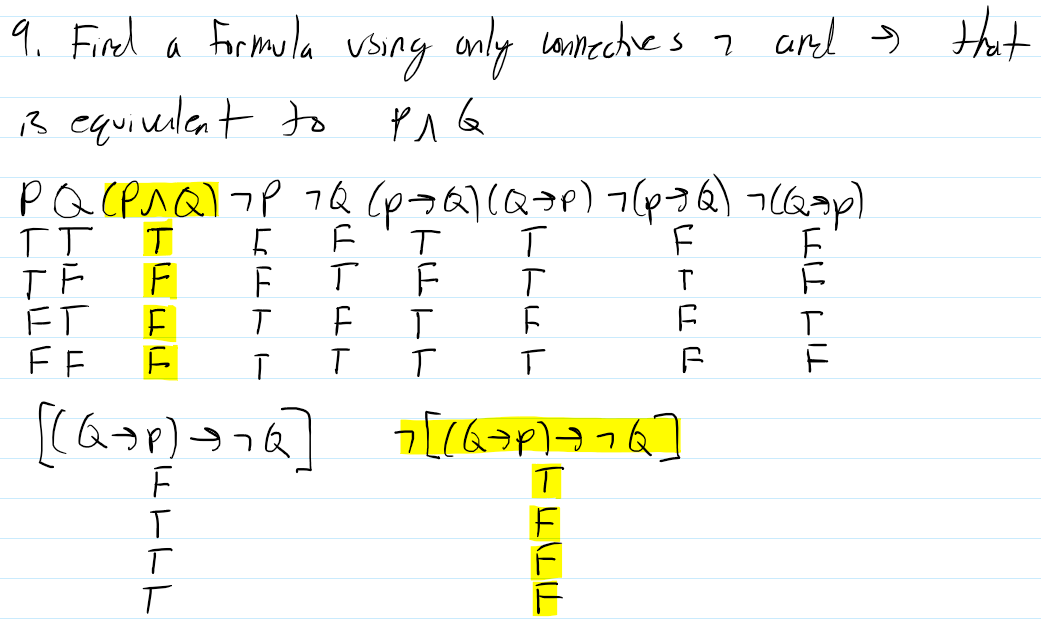
\includegraphics[width=0.8\textwidth]{images/1.2/33.PNG}
\end{figure}

\textbf{Solution}
\begin{align*}
(P \rightarrow Q) \wedge P &\equiv (\neg P \vee Q) \wedge P && \quad \text{def. of $\rightarrow$}\\
&\equiv (P \wedge \neg P) \vee (P \wedge Q) && \quad \text{distributive} \\
&\equiv (P \wedge Q) && \quad \text{idempotent}
\end{align*}

\textbf{Problem 10:}
\begin{figure}[H]
    \centering
    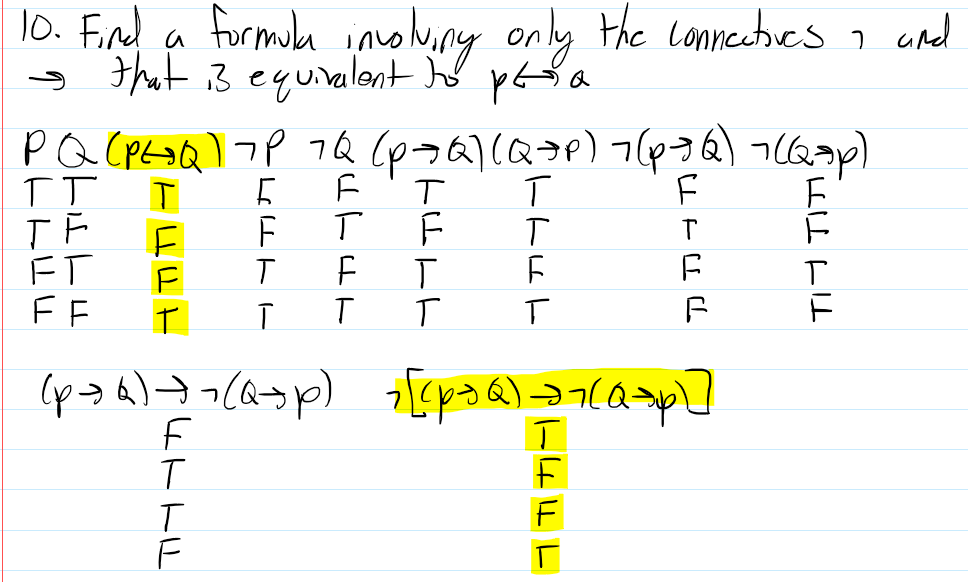
\includegraphics[width=0.8\textwidth]{images/1.2/34.PNG}
\end{figure}

\textbf{Problem 11:}
\begin{figure}[H]
    \centering
    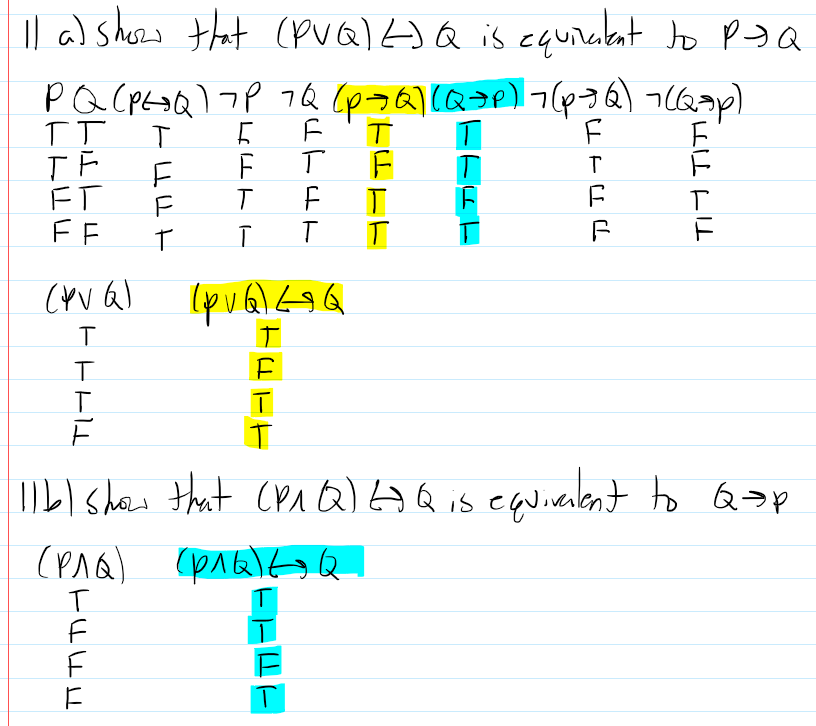
\includegraphics[width=0.8\textwidth]{images/1.2/35.PNG}
\end{figure}

\textbf{Problem 12:}
\begin{figure}[H]
    \centering
    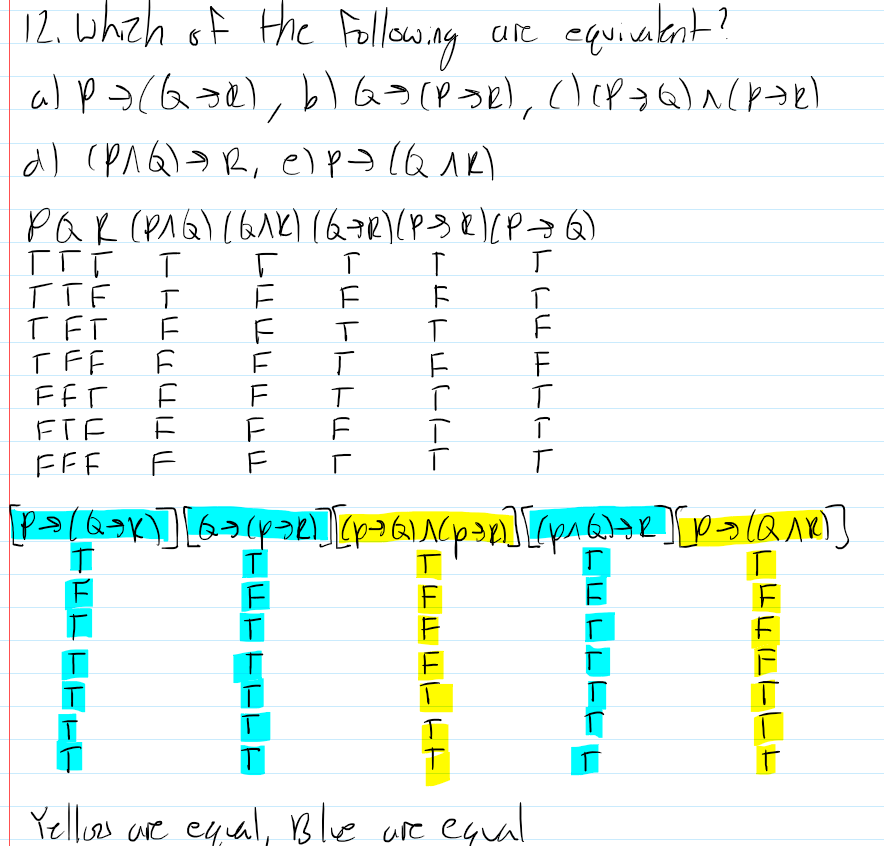
\includegraphics[width=0.8\textwidth]{images/1.2/36.PNG}
\end{figure}